% =====================================================================
%  Semester thesis — X. Lu, TUM CIT, Chair of Robotics, Artificial
%  Intelligence and Real-time Systems (Prof. Knoll)
%  Layout follows the TUM CIT thesis look (Charter body, Helvetica
%  headings, TUM blue title page). Build:  latexmk -pdf main.tex
% =====================================================================
\documentclass[11pt,a4paper,oneside,chapterprefix=true,headings=big,parskip=false,numbers=noenddot,bibliography=totoc,listof=totoc]{scrreprt}

% ---------- fonts and language ----------
\usepackage[T1]{fontenc}
\usepackage[utf8]{inputenc}
\usepackage[charter]{mathdesign}
\usepackage[scaled=0.92]{helvet}
\usepackage[english]{babel}
\usepackage{microtype}

% ---------- page geometry and headers ----------
\usepackage[a4paper,left=30mm,right=30mm,top=32mm,bottom=32mm,headsep=10mm]{geometry}
\usepackage[automark,headsepline=false]{scrlayer-scrpage}
\clearpairofpagestyles
\ihead{\sffamily\itshape\small\headmark}
\ohead{\sffamily\bfseries\small\pagemark}
\renewcommand*{\chaptermarkformat}{}
\automark[section]{chapter}
\setkomafont{pageheadfoot}{\normalfont}
\setkomafont{disposition}{\sffamily\bfseries}
\setkomafont{chapterprefix}{\huge}
\renewcommand*{\chapterformat}{\chapapp~\thechapter\autodot}
\RedeclareSectionCommand[beforeskip=40mm,afterskip=18mm,innerskip=10mm]{chapter}
\RedeclareSectionCommand[beforeskip=-4ex plus -1ex minus -.2ex,afterskip=2.2ex]{section}

% ---------- math, units, tables, figures ----------
\usepackage{amsmath}
\usepackage{bm}
\usepackage{siunitx}
\sisetup{per-mode=power,range-phrase=\,--\,,range-units=single,detect-all}
\usepackage{booktabs,tabularx,multirow,array}
\usepackage{graphicx}
\graphicspath{{figures/}}
\usepackage[font=small,labelfont={bf,sf},format=hang]{caption}
\usepackage{subcaption}
\usepackage{float}
\usepackage{xcolor}
\definecolor{TUMblue}{HTML}{0065BD}
\definecolor{todo}{HTML}{C0392B}
\usepackage{tikz}
\usetikzlibrary{arrows.meta,positioning,calc,fit,backgrounds,decorations.pathmorphing,patterns}
\usepackage{enumitem}
\setlist{itemsep=2pt,topsep=4pt}
\usepackage{csquotes}

% ---------- bibliography ----------
\usepackage[backend=biber,style=alphabetic,maxbibnames=99,maxcitenames=2,giveninits=true,doi=true,url=false,isbn=false,eprint=true]{biblatex}
\addbibresource{refs.bib}
\AtEveryBibitem{\clearfield{note}}

% ---------- cross references ----------
\usepackage[hidelinks,pdfusetitle]{hyperref}
\usepackage[capitalise,noabbrev,nameinlink]{cleveref}

% ---------- helpers ----------
\setlength{\emergencystretch}{3em}
\newcommand{\TODO}[1]{\textcolor{todo}{\textbf{[TODO:} #1\textbf{]}}}
\newcommand{\U}{U}                          % swimming / tow speed
\newcommand{\Tm}{\bar{T}}                   % cycle-mean thrust
\newcommand{\Pm}{\bar{P}}                   % cycle-mean input power
\newcommand{\etaF}{\eta}                    % Froude efficiency
\newcommand{\mNs}{\si{\milli\newton}}
\newcommand{\ms}{\si{\metre\per\second}}
\newcommand{\sfit}[1]{\textsf{#1}}

% ---------- title data ----------
\newcommand{\thesistype}{Semester Thesis in Mechatronics, Robotics, and Biomechanical Engineering}
\newcommand{\thesistitle}{Hydrodynamic Modeling and Trajectory Optimization of Paddling Propulsion for a Quadruped Robot}
\newcommand{\thesisauthor}{Xiaotian Lu}
\newcommand{\thesissupervisor}{Prof.\ Dr.-Ing.\ habil.\ Alois C.\ Knoll}
\newcommand{\thesisadvisor}{Qian Huang, M.Sc.}
\newcommand{\thesisdate}{October 2026}      % TODO: submission date
\hypersetup{pdftitle={\thesistitle},pdfauthor={\thesisauthor}}

\begin{document}
\pagenumbering{roman}
% ---------------- title page (TUM CIT look) ----------------
\begin{titlepage}
\newgeometry{left=25mm,right=25mm,top=20mm,bottom=25mm}
\sffamily
\begin{minipage}[t]{0.7\textwidth}
  {\color{TUMblue}\small TUM School of Computation, Information and Technology\\
  Technical University of Munich}
\end{minipage}\hfill
\begin{minipage}[t]{0.25\textwidth}\raggedleft
  % Insert the official TUM logo from the university template here:
  \IfFileExists{figures/tum_logo.pdf}{
\includegraphics[height=10.5mm]{tum_logo}}{\color{TUMblue}\fbox{\parbox[c][10mm][c]{24mm}{\centering\tiny TUM logo\\(from template)}}}
\end{minipage}

\vspace*{75mm}
{\large \thesistype\par}
\vspace{8mm}
{\noindent\raggedright\hyphenpenalty=10000\color{TUMblue}\bfseries\fontsize{22}{27}\selectfont \thesistitle\par}
\vfill
\begin{tabular}{@{}p{45mm}l}
\textbf{Supervisor} & \thesissupervisor\\[3mm]
\textbf{Advisor}    & \thesisadvisor\\[3mm]
\textbf{Author}     & \thesisauthor\\[3mm]
\textbf{Date}       & \thesisdate{} in Munich
\end{tabular}
\restoregeometry
\end{titlepage}

\thispagestyle{empty}
\vspace*{40mm}
\noindent{\sffamily\bfseries\LARGE Disclaimer\par}
\vspace{14mm}
\noindent I confirm that this semester thesis is my own work and I have documented all sources and material used.
The author used Claude (Anthropic) to assist with data post-processing scripts, figure generation and language
refinement during the preparation of this manuscript. All AI-assisted text and code were critically reviewed,
revised, and verified by the author. All technical ideas, simulation set-ups, analyses, results, figure content,
and conclusions were developed and verified by the author.

\vspace{25mm}
\noindent Munich, \thesisdate\hfill\begin{tabular}[t]{c}\rule{60mm}{0.4pt}\\ \footnotesize(\thesisauthor)\end{tabular}
\cleardoublepage

\thispagestyle{empty}
\vspace*{25mm}
\noindent{\sffamily\bfseries\Large Abstract\par}
\vspace{6mm}
\noindent
Amphibious quadruped robots can swim by moving their legs, but a leg designed for walking makes a poor
propulsor. This thesis asks which propulsion principle suits the legs of the quadruped BODY2 and how each
propulsor should move. Drag-based paddling with a folding fan paddle is compared with lift-based flapping of a
small fluke fitted to the same leg. Three simulation tools with different roles are used. First, a reduced-order
MuJoCo model with Morison-type link forces and an actuator speed limit is combined with CMA-ES gait
optimization. Whenever the model contains lift and lift is not suppressed, every feasible optimized gait is lift-propelled, and at equal speed the lift gaits
need one half to one third of the power of the best gaits of a drag-only model. Second, the single leg is simulated
with overset-grid CFD in OpenFOAM. For the fan paddle, a trapezoidal velocity law, a 12-mm folded width and
closing the fan at the start of the deceleration raise the thrust from \SI{23.4}{\milli\newton} for the robot's
current gait to \SIrange{73}{83}{\milli\newton} per leg at rest; the range bounds the change of added mass at the
fold, which the two-state model of the folding fan does not resolve. The paddle loses its thrust by about
\SI{0.30}{\metre\per\second}, because its recovery drag and the cost of opening the fan in the oncoming flow grow
while its power-stroke thrust decays. The fluke produces the same thrust per area at rest and loses it more slowly with speed.
Thrust and efficiency cross over at about \SI{0.24}{} and \SI{0.22}{\metre\per\second}. Scheduling the fluke pitch with speed keeps the angle of attack near
\SI{20}{\degree} and raises the Froude efficiency at \SI{0.30}{\metre\per\second} from 0.24 to 0.40. A
quasi-steady self-propulsion balance predicts a cruising speed of \SI{0.30}{\metre\per\second} for the fluke and
\SIrange{0.26}{0.27}{\metre\per\second} for the optimized paddle, with 43\,\% less power for the fluke with
speed-scheduled pitch. A first hardware test with flukes at \SI{2}{\hertz} is 1.3 to 1.6 times slower than predicted, so these
speeds are upper bounds for the present robot. Third, the real-time solver Flare Live supplies the reference fluke motion, but its lattice does not resolve the
foil and it underpredicts the fluke thrust, so it is used for trends only. The CFD set-up
reproduces the thrust coefficient of a flapping-foil experiment to within 8\,\%.

\vspace{12mm}
\noindent{\sffamily\bfseries\Large Kurzfassung\par}
\vspace{6mm}
\noindent\begingroup\sisetup{locale=DE}
Amphibische Vierbeiner können schwimmen, indem sie ihre Beine bewegen, doch ein zum Laufen ausgelegtes Bein
ist ein schlechter Antrieb. Diese Arbeit untersucht, welches Antriebsprinzip zu den Beinen des Vierbeiners
BODY2 passt und wie sich der jeweilige Antrieb bewegen sollte. Verglichen werden widerstandsbasiertes Paddeln
mit einem faltbaren Fächerpaddel und auftriebsbasiertes Schlagen mit einer kleinen Flosse am selben Bein. Dazu
werden drei Simulationswerkzeuge mit unterschiedlichen Aufgaben eingesetzt. Zunächst wird ein Modell reduzierter Ordnung in
MuJoCo mit Morison-Kräften je Glied und begrenzter Stellgeschwindigkeit der Servos mit einer CMA-ES-Gangoptimierung kombiniert.
Sobald das Modell Auftrieb enthält und dieser nicht unterdrückt wird, nutzen alle zulässigen optimierten Gangarten Auftrieb, und bei gleicher Geschwindigkeit benötigen
sie nur die Hälfte bis ein Drittel der Leistung der besten Gangarten eines reinen Widerstandsmodells. Anschließend
wird das Einzelbein mit Overset-CFD in OpenFOAM simuliert. Für das Fächerpaddel erhöhen ein trapezförmiges
Geschwindigkeitsprofil, eine gefaltete Breite von 12\,mm und das Schließen des Fächers zu Beginn der
Verzögerung den Schub im Stand von \SI{23.4}{\milli\newton} (aktueller Gang des Roboters) auf
\SIrange{73}{83}{\milli\newton} pro Bein; die Spanne erfasst die Änderung der hydrodynamischen Masse beim Falten, die das
Zwei-Zustands-Modell des Fächers nicht auflöst. Bei etwa \SI{0.30}{\metre\per\second} verliert das Paddel seinen Schub, weil
Rückholwiderstand und der Aufwand zum Öffnen des Fächers in der Anströmung wachsen, während der Schub im Arbeitshub abnimmt.
Die Flosse erzeugt im Stand denselben Schub pro Fläche und verliert ihn mit der Geschwindigkeit langsamer. Schub und Wirkungsgrad kreuzen sich bei etwa
\SI{0.24}{} bzw. \SI{0.22}{\metre\per\second}.
Eine geschwindigkeitsabhängige Anstellung hält den Anstellwinkel bei etwa \SI{20}{\degree} und steigert den
Froude-Wirkungsgrad bei \SI{0.30}{\metre\per\second} von 0,24 auf 0,40. Eine quasistationäre
Eigenantriebsbilanz sagt für die Flosse \SI{0.30}{\metre\per\second} und für das optimierte Paddel
\SIrange{0.26}{0.27}{\metre\per\second} voraus, wobei die Flosse mit geschwindigkeitsabhängiger Anstellung 43\,\% weniger
Leistung benötigt. Ein erster Schwimmversuch des Roboters mit Flossen ist bei \SI{2}{\hertz} 1,3- bis 1,6-mal langsamer als
vorhergesagt; die vorhergesagten Geschwindigkeiten sind daher Obergrenzen für den aktuellen Roboter. Der Echtzeitlöser Flare Live
liefert die Referenzbewegung der Flosse, löst das Profil jedoch nicht auf und unterschätzt den Flossenschub; er dient daher nur zur
Einordnung von Trends. Der CFD-Aufbau gibt den Schubbeiwert eines Schlagflügelexperiments auf 8\,\% genau wieder.\endgroup
\cleardoublepage

\pagestyle{scrheadings}
\tableofcontents
\listoffigures
\listoftables
\chapter*{List of Acronyms and Symbols}
\addcontentsline{toc}{chapter}{List of Acronyms and Symbols}
\markboth{List of Acronyms and Symbols}{List of Acronyms and Symbols}

\begin{description}[labelwidth=16mm,leftmargin=20mm,itemsep=1pt,font=\normalfont\bfseries]
\item[AR] aspect ratio, $\mathit{AR}=b^2/S$
\item[BL] body length (speeds in BL/s)
\item[CFD] computational fluid dynamics
\item[CMA-ES] covariance matrix adaptation evolution strategy
\item[COT] cost of transport
\item[EMF] electromotive force (back-EMF of the servo motor)
\item[GCI] grid convergence index
\item[LSTM] long short-term memory (recurrent neural network)
\item[MJCF] MuJoCo XML model format
\item[PIMPLE] merged PISO--SIMPLE pressure--velocity coupling algorithm
\item[RMS] root mean square
\item[SPH] smoothed-particle hydrodynamics
\item[URDF] unified robot description format
\end{description}

\bigskip
\begin{description}[labelwidth=16mm,leftmargin=20mm,itemsep=1pt,font=\normalfont]
\item[$\U$] forward (swimming or tow) speed, \si{\metre\per\second}
\item[$f,\;T$] stroke frequency and period, $T=1/f$
\item[$\tau$] cycle phase $t/T\bmod 1$
\item[$\Tm$] cycle-mean thrust of one leg, \si{\milli\newton}
\item[$\Pm$] cycle-mean hydrodynamic input power of one leg, \si{\milli\watt}
\item[$\etaF$] Froude efficiency $\Tm\U/\Pm$
\item[$C_T$] thrust coefficient $\Tm/(\tfrac12\rho\U^2S)$
\item[$\mathit{St}$] Strouhal number $fA/\U$ with peak-to-peak excursion $A$
\item[$\alpha$] angle of attack between foil chord and relative inflow
\item[$\gamma$] inflow angle of the heaving foil, $\gamma=\arctan(\dot h/\U)$
\item[$\theta$] fluke pitch angle
\item[$\mathrm{DUTY}$] fraction of the cycle spent in the power stroke
\item[$\tau_o,\tau_c$] phases at which the fan paddle is opened and closed
\item[$K$] hull drag coefficient in $D=K\U|\U|$, \si{\newton\second\squared\per\metre\squared}
\item[$\rho,\nu$] density and kinematic viscosity of water
\end{description}

\bigskip
\noindent\textbf{Case names}
\begin{description}[labelwidth=16mm,leftmargin=20mm,itemsep=1pt,font=\normalfont\bfseries]
\item[Robot gait] fan paddle with the robot's current stroke (\SI{1.25}{\second} period, fold to \SI{30}{\milli\metre})
\item[V1--V3] design steps of the drag-type stroke at rest; V3trap: the optimized stroke (trapezoidal velocity law, fold to \SI{12}{\milli\metre}, early closing)
\item[L0] fluke with the reference motion from Flare Live at \SI{0.223}{\metre\per\second}; L0c: the same on the coarse mesh
\item[L2] L0 motion at other speeds (\SIlist{0;0.08;0.15;0.30}{\metre\per\second})
\item[L1] fluke with an angle-of-attack law (L1a10, L1a28: targets of \SI{10}{} and \SI{28}{\degree})
\item[L3] fluke with the speed-scheduled pitch $\theta_0=\gamma_\text{max}/2$ (L3U030, L3U040 at \SI{0.30}{} and \SI{0.40}{\metre\per\second})
\item[Validation] heaving and pitching NACA\,0012 foil after Schouveiler et al.\ (\cref{sec:ver-v1})
\end{description}


\cleardoublepage
\pagenumbering{arabic}
\chapter{Introduction}
\label{ch:intro}

\section{Motivation}

Legged robots move well on land, and many of the places where they are useful, such as shorelines, flooded
areas, ponds and river banks, also contain open water. A quadruped that crosses such water needs some way to
propel itself when its feet no longer touch the ground. Adding thrusters is one option \cite{Yao2023}, but
thrusters add mass, volume and actuators that are useless on land. The alternative is to swim with the legs
themselves \cite{Li2019,Qu2025,Han2025,Wang2025}. Then no extra hardware is needed, and swimming becomes a
question of how the existing joints are moved and what the feet look like.

Animals that swim with legs use two different physical principles \cite{Fish1996}. A dog, a muskrat or a duck
\emph{paddles}. It pushes water backwards with a foot oriented normal to its motion and then brings the foot
forward again \cite{Fish1984,Fish2021DogPaddle}. The thrust comes from drag on the foot during the power
stroke, and the recovery stroke unavoidably costs some thrust. Dolphins, sea turtles and many fish instead
\emph{flap} a fin or fluke across the swimming direction. The fin meets the oncoming water at a small angle of
attack and produces lift, whose forward component is the thrust. Drag-based paddling is simple, works at rest
and accelerates well. Lift-based flapping is two to three times more efficient at cruising speed
\cite{Fish1996,Walker2000}. Mammals that became fully aquatic changed over from the first principle to the
second.

Most swimming legged robots use the first principle, because a walking foot is already a paddle. This thesis
studies whether that choice is right for a small amphibious quadruped, BODY2, and how the leg should move for
each principle. The robot's legs were designed for walking. Each is a planar two-degree-of-freedom linkage
driven by two hobby servos, and the foot is a fan-shaped paddle that folds during the recovery stroke. Its
current swimming gait was taken from video of the robot and has not been designed for thrust. Whether this
paddle can be made efficient, or whether a small lift-producing fluke on the same leg would be better, cannot
be decided from the literature alone, because the answer depends on the leg geometry, the actuator limits and
the swimming speed.

\section{Problem Statement and Scope}

The problem is to find, for a given leg and given actuators, the propulsor and the periodic leg motion that
propel the robot most effectively, and to quantify how the answer depends on swimming speed. Three
properties make the problem difficult.

First, the flow is unsteady and separated. A paddle starts and stops twice per cycle, sheds a vortex at every
stop, and meets its own wake. A flapping fluke works at Reynolds numbers of $10^3$--$10^4$, where
leading-edge vortices and the phase between heave and pitch decide the thrust
\cite{Triantafyllou1991,Anderson1998}. Quasi-steady models capture trends but not the magnitudes of these
effects \cite{Kim2011}.

Second, the answer depends on speed. At rest, a paddle pushes water that is not moving and produces thrust
over most of its power stroke. At speed, the oncoming flow reduces the relative velocity during the power
stroke and increases it during the recovery. A lift-based foil behaves in the opposite way: its angle of
attack is set by the ratio of heave velocity to swimming speed, so it depends on speed through the kinematics.
A comparison at a single speed can therefore favour either principle.

Third, no single model is both accurate and cheap. A three-dimensional CFD simulation of one leg takes hours to
days and cannot be placed inside an optimizer that needs thousands of evaluations. A reduced-order model can,
but its coefficients are not calibrated and its lift model is a textbook flat plate.

Three simulation tools are therefore used, each for a different question, and none is expected to reproduce the
numbers of the others:
\begin{itemize}
  \item a \emph{reduced-order} whole-robot model in MuJoCo with CMA-ES gait optimization answers a question of
        \emph{mechanism}: which propulsion principle does an optimizer select under actuator and stability constraints? Its
        coefficients are not calibrated, so it is used for direction, not for magnitude;
  \item \emph{single-leg CFD} of the real BODY2 leg geometry in OpenFOAM with overset grids answers the questions of
        \emph{magnitude}: how much thrust and power each propulsor produces across forward speed, and where one overtakes the
        other. It is validated against an experiment and provides every quantitative result of this thesis;
  \item the \emph{whole-robot} real-time solver Flare Live provides the reference fluke motion. Its fluke force is checked against
        the CFD and found too low, so its results are used for trends only.
\end{itemize}
\Cref{fig:overview} shows how the three tools and their results are connected. Where the reduced-order model and the CFD
disagree, the CFD is authoritative; the disagreement itself is analysed in \cref{sec:disc-models}.

\begin{figure}[t]
  \centering
  \begin{tikzpicture}[>=Latex,font=\small,
      box/.style={draw=TUMblue,thick,rounded corners=2pt,align=center,inner sep=4pt,text width=35mm,minimum height=17mm,fill=TUMblue!6,execute at begin node={\hyphenpenalty=10000\relax}},
      res/.style={draw=black!45,rounded corners=2pt,align=center,inner sep=3pt,text width=35mm,minimum height=9mm,fill=black!3,font=\footnotesize,execute at begin node={\hyphenpenalty=10000\relax}},
      lab/.style={font=\footnotesize\itshape,text=black!60}]
    \node[box,font=\small] (mj) at (0,0) {\textbf{Reduced-order model}\\MuJoCo, Morison\\forces, servo model,\\CMA-ES (\cref{ch:mujoco})};
    \node[box] (cfd) at (5.1,0) {\textbf{Single-leg CFD}\\OpenFOAM, overset grids,\\real leg geometry\\(\cref{ch:cfd,ch:verification})};
    \node[box] (fl) at (10.2,0) {\textbf{Whole-robot model}\\Flare Live, lattice\\Boltzmann, real time\\(\cref{sec:cfd-flare})};
    \node[lab,above=1pt of mj.north] {fast, uncalibrated};
    \node[lab,above=1pt of cfd.north] {resolved, validated};
    \node[lab,above=1pt of fl.north] {whole robot, coarse};
    \node[res] (r1) at (0,-2.3) {mechanism: which principle\\an optimizer selects (RQ1)};
    \node[res] (r2) at (5.1,-2.3) {thrust, power, efficiency\\vs.\ speed; crossover (RQ2)};
    \node[res] (r3) at (10.2,-2.3) {cross-check of the fluke force (\cref{sec:ver-flare})};
    \node[res] (sp) at (5.1,-4.2) {self-propulsion estimate $4\bar T(U)=D(U)$ (RQ3)};
    \node[res] (hw) at (10.2,-4.2) {first hardware test\\(\cref{sec:res-hw})};
    \draw[->] (mj) -- (r1); \draw[->] (cfd) -- (r2); \draw[->] (fl) -- (r3); \draw[->] (r2) -- (sp);
    \draw[->,dashed] (mj.east) -- node[above,lab,fill=white,inner sep=1pt]{lift?} (cfd.west);
    \draw[->,dashed] (fl.west) -- node[above,lab,fill=white,inner sep=1pt]{L0 motion} (cfd.east);
    \draw[->,dashed] (r2.east) -- node[above,lab,fill=white,inner sep=1pt]{fluke force} (r3.west);
    \draw[<->,dashed] (sp.east) -- node[above,lab,fill=white,inner sep=1pt]{compare} (hw.west);
  \end{tikzpicture}
  \caption[Overview of the method]{Overview of the three simulation tools and their roles. Solid arrows: results; dashed arrows:
    information passed between tools. The reduced-order model motivates the lift-type propulsor, Flare Live provides the reference fluke motion, and the CFD
    provides the thrust curves for the self-propulsion estimate and the reference against which the Flare Live fluke force is checked.}
  \label{fig:overview}
\end{figure}

The scope is limited as follows.
\begin{itemize}
  \item \emph{Environment.} The robot swims at the surface of still water. Waves, currents and the transition
        between land and water are excluded. All propulsor CFD is single-phase with a rigid lid; the free surface is
        not modelled.
  \item \emph{Motion.} Only steady, periodic, straight-ahead swimming is considered. Turning, starting and
        feedback control are excluded.
  \item \emph{Propulsors.} Two propulsors fitted to the same leg are compared: the robot's folding fan paddle
        (drag-based) and a small swept fluke on a pin joint (lift-based). The fluke pitch is prescribed in
        the simulations; the passive pin-and-spring realization of the hardware is not simulated.
  \item \emph{Evaluation.} Thrust and hydrodynamic input power are computed for the propulsor alone (fan or
        fluke), without the linkage. Swimming speeds are predicted from a quasi-steady force balance with a
        range of hull resistances. Hardware experiments are limited to a first timed test from rest.
\end{itemize}

\section{Research Questions and Hypotheses}

The central question of this thesis is:
\begin{quote}
\itshape Which propulsion principle, drag-based paddling or lift-based flapping, lets the legs of BODY2 swim
faster and more efficiently, and how should each propulsor move?
\end{quote}
It is split into three research questions, each paired with a hypothesis.

\begin{description}[leftmargin=12mm,style=nextline]
\item[(RQ1)] \emph{Reduced-order optimization.} When a whole-robot gait is optimized in a reduced-order
  hydrodynamic model under actuator-speed and attitude limits, which propulsion mechanism does the optimizer
  select, and does the answer depend on the physics included in the model?

  \emph{Hypothesis H1.} If the model contains a lift term, the optimizer uses lift-based strokes, and at equal
  speed these need less power than drag-based strokes.

\item[(RQ2)] \emph{Drag versus lift across speed.} For the real leg geometry, how large are thrust, power and
  Froude efficiency of an optimized drag-type paddle and of a lift-type fluke between rest and
  \SI{0.4}{\metre\per\second}, and what limits each propulsor?

  \emph{Hypothesis H2.} The optimized paddle produces more thrust at low speed, but its thrust falls steeply
  with speed because the recovery stroke meets an increasing oncoming flow. The fluke produces less thrust at
  rest, keeps a larger fraction at speed, and becomes both stronger and more efficient above a crossover
  speed. The fluke performs best when its pitch is adapted to the speed so that the angle of attack stays
  near the efficient range of flapping foils (about \SIrange{15}{25}{\degree}).

\item[(RQ3)] \emph{Whole robot.} What cruising speed and power follow for the whole robot?

  \emph{Hypothesis H3.} Both optimized propulsors reach similar cruising speeds, set by the hull and linkage
  resistance, but the fluke needs less power.
\end{description}

RQ1 is answered in \cref{ch:mujoco}. RQ2 and RQ3 are answered in \cref{ch:results}, after the CFD method and
its verification in \cref{ch:cfd,ch:verification}. \Cref{ch:discussion} evaluates the hypotheses.

\section{Contributions}

The contributions of this thesis are:
\begin{enumerate}
  \item \emph{A reduced-order gait-optimization pipeline with an actuator model} (\cref{ch:mujoco}).
        Morison-type link forces with an optional flat-plate lift term, a DC-motor torque--speed model of
        the servos and feasibility-first constraints are combined with CMA-ES. In all 101 feasible optima
        obtained with lift in the model and without a limit on the lift share, lift supplies the forward impulse and drag opposes it. A lift-share limit
        allows drag-based and lift-based strokes to be compared within the same model.
  \item \emph{An optimized drag-type stroke for the BODY2 fan paddle} (\cref{sec:res-drag}). Overset CFD of the
        real leg with a two-state composite for the folding fan yields a stroke with a trapezoidal velocity
        law, a 12-mm folded width and early closing that produces \SIrange{73}{83}{\milli\newton} per leg
        at rest, 3.1--3.5 times the robot's current gait. The added-mass change that the composite does not resolve
        is bounded analytically with an added mass identified from the CFD.
  \item \emph{A speed-resolved comparison of drag- and lift-type propulsors on the same leg}
        (\cref{sec:res-compare}). Thrust, power and efficiency are computed from rest to
        \SI{0.40}{\metre\per\second}. The drag paddle's speed limit is traced to its recovery, the
        thrust and efficiency crossovers are located at about \SI{0.24}{} and \SI{0.22}{\metre\per\second}, and a speed-scheduled
        fluke pitch raises the fluke efficiency at \SI{0.30}{\metre\per\second} from 0.24 to 0.40.
  \item \emph{Self-propulsion estimates and a fidelity assessment} (\cref{sec:res-selfprop,ch:verification}).
        Cruising speeds are bounded with a range of hull resistances, the CFD set-up is validated against
        a flapping-foil experiment and checked for mesh and cycle convergence, and the thrust deficit of
        the real-time solver Flare Live is quantified on the same fluke motion.
\end{enumerate}

\section{Thesis Outline}

\Cref{ch:related} reviews drag- and lift-based swimming in animals and robots, flapping-foil hydrodynamics
and simulation approaches for swimming legged robots. \Cref{ch:foundations} introduces the quantities and
simple models used throughout: quasi-steady paddling, flapping-foil kinematics and the self-propulsion
balance. \Cref{ch:platform} describes the robot, the two propulsors and their leg motions.
\Cref{ch:mujoco} presents the reduced-order model and the gait optimization. \Cref{ch:cfd} describes the
single-leg CFD and the whole-robot Flare Live model, and \cref{ch:verification} verifies and validates the CFD and
checks the real-time solver against it. \Cref{ch:results} reports the drag-type stroke design, the lift-type fluke,
their comparison, the speed schedule for the fluke pitch and the self-propulsion estimates.
\Cref{ch:discussion} interprets the results and states the limitations, and \cref{ch:conclusion} concludes
and outlines future work. The appendices collect additional data, the coordination results of the reduced-order model
(\cref{app:coord}), the Flare Live results (\cref{app:flare-trends}) and information for reproducing the work.

\chapter{Related Work}
\label{ch:related}

This chapter reviews what is known about drag- and lift-based swimming in animals and on foils, how swimming
legged robots have been designed and simulated, and which gap this thesis addresses.

\section{Drag- and Lift-Based Swimming in Animals}
\label{sec:rw-bio}

Fish \cite{Fish1996} classified mammalian swimming by the force that produces thrust. Paddlers such as the
muskrat, mink or dog move a foot or hand backwards against the water in a power stroke and return it in a
recovery stroke. Their propulsive efficiency is at most about 0.33. Swimmers that oscillate a fluke or flipper
across the swimming direction generate lift and reach efficiencies above 0.8. Fish argued that the transition
from paddling to lift-based swimming in the evolution of aquatic mammals was driven by this efficiency
difference and that intermediate forms combine both principles.

The muskrat is the best-documented paddler \cite{Fish1984}. Its power stroke lasts \SI{0.18}{\second} and
its recovery \SI{0.22}{\second}, a duty factor of 0.45. During recovery it folds the toes together, reducing
the frontal area of the foot by 55.5\,\%, yet the recovery drag still amounts to about one third of the
power-stroke thrust. Its maximum mechanical efficiency is 0.33. Dogs use a stereotyped diagonal paddling
gait, in which each foot moves on a closed path and the fore- and hindlimbs of opposite sides move together
\cite{Fish2021DogPaddle}. Ducks paddle with webbed feet whose hydrodynamic performance resembles that of oars
rather than delta wings \cite{Ribak2023}.

Cetaceans are the reference for lift-based swimming. Bottlenose dolphins swim with a propulsive efficiency
of about 0.8 \cite{Fish1993}. Odontocetes cruise at Strouhal numbers of $0.26\pm0.05$ \cite{Rohr2004}, and
flying and swimming animals in general cruise at $0.2<\mathit{St}<0.4$, the range of high power efficiency of
oscillating foils \cite{Taylor2003}. Walker and Westneat \cite{Walker2000} compared rowing and flapping
appendages with a blade-element model and concluded that rowing is favourable at low speeds and for
manoeuvres and acceleration, whereas flapping is more efficient at higher speeds. For BODY2 this suggests the division of
labour tested in this thesis, a paddle for starting and low speed and a fluke for cruising, and makes the speed at which one
overtakes the other the quantity to be found.

\section{Flapping-Foil Hydrodynamics}
\label{sec:rw-foil}

A foil that heaves and pitches with a phase difference produces thrust through a leading-edge vortex on each
half stroke and a reverse von K\'arm\'an street in its wake \cite{Triantafyllou1991}. Wake stability analysis
predicts the highest efficiency at $0.25\lesssim\mathit{St}\lesssim0.35$ \cite{Triantafyllou1991}. Anderson et
al.\ \cite{Anderson1998} measured efficiencies up to 0.87 for a NACA\,0012 foil at a heave amplitude of
$0.75$ chord, a maximum angle of attack of about \SI{20}{\degree} and a pitch lead of \SI{75}{\degree}. Read
et al.\ \cite{Read2003} extended these measurements and found a broad efficiency plateau of 0.5--0.6 for
maximum angles of attack between \SI{15}{\degree} and \SI{25}{\degree} and the largest thrust coefficients,
around 2.4, at $\mathit{St}\approx0.6$ and angles of attack of \SIrange{30}{35}{\degree}, where efficiency drops
to below 0.5. Hover et al.\ \cite{Hover2004} showed that the time history of the angle of attack matters as
much as its maximum: an angle of attack held nearly constant over the stroke extends the efficient range to
higher Strouhal numbers and thrust. Schouveiler et al.\ \cite{Schouveiler2005} reported thrust coefficients
and efficiencies with error bars over a range of Strouhal numbers and angles of attack; one of their points
is used as the validation case in \cref{sec:ver-v1}. Floryan et al.\ \cite{Floryan2017} derived scaling laws
in which thrust grows with the square of the Strouhal number and efficiency favours large amplitudes at low
frequencies. For a self-propelled swimmer, the Strouhal number is not a free parameter but follows from the
balance of thrust and drag \cite{Eloy2012}. Three-dimensional effects reduce thrust at low aspect ratio;
cetacean flukes have aspect ratios of about 2--6 \cite{Ayancik2020}. For the fluke of BODY2 these results fix the target: an
angle of attack of about \SIrange{15}{25}{\degree} and a Strouhal number of 0.2--0.4, which its pitch must maintain while the
swimming speed changes.

\section{Paddling Mechanics}
\label{sec:rw-paddle}

A paddle produces net thrust only through an asymmetry between power and recovery stroke, either spatial
(a smaller area during recovery) or temporal (a slower recovery) \cite{HerreraAmaya2024}. Kim and Gharib
\cite{Kim2011} measured the flow around a flat plate performing a paddling rotation and showed that the thrust
follows the growth and shedding of the starting vortex rather than the quasi-steady square of the plate
velocity. Crustacean-inspired propulsors reach their best performance when the appendage opens quickly at
the start of the power stroke and closes early in the recovery \cite{Santos2026}. A tendon coupling that
shortens the transition between the open and folded states of a webbed robotic foot doubled its propulsive
efficiency \cite{Lin2024}. For beaver-like robots, the hydrodynamics of bendable webbed feet have been modelled
with quasi-steady methods and measured in flumes \cite{Chen2021,Chen2022}. For the fan paddle of BODY2 the levers are therefore
the folded area, the timing of the fold and the velocity law of the power stroke; all three are varied in \cref{sec:res-drag}.

\section{Swimming Legged Robots}
\label{sec:rw-robots}

Picardi et al.\ \cite{Picardi2023} reviewed underwater legged robots; most walk on the bottom and few swim.
Li et al.\ \cite{Li2019} analysed the kinematics and hydrodynamics of a robotic dog paddling with rigid
limbs. Qu et al.\ \cite{Qu2025} built an amphibious robotic dog and measured single-leg and whole-robot
thrust for paddling gaits with different power-stroke fractions; a shorter power stroke produced more thrust
but also larger roll. Wang et al.\ \cite{Wang2025} simulated quadrupedal paddling with an immersed-boundary
CFD solver. They varied the initial swing angle, the swing amplitude and the power-stroke fraction of rigid,
non-folding legs at zero forward speed, and found that the thrust of four legs exceeds four times the
single-leg thrust by up to 87\,\%. Han et al.\ \cite{Han2025} trained an LSTM model of the leg forces from
tank measurements and used it for multi-objective gait optimization. Yao et al.\ \cite{Yao2023} instead added
thrusters to a quadruped and learned a propulsion controller.

Lift-based propulsion has been demonstrated on robots with dedicated flippers. Baines et al.\
\cite{Baines2022} built a turtle robot with morphing limbs that can paddle and flap with the same limb; the
flapping gait produced thrust over most of the stroke and had the lower cost of transport, while paddling
gave higher accelerations. The DuckyDog robot uses variable-stiffness legs with passive fins
\cite{Wang2025DuckyDog}. Within the same chair as this thesis, Heber \cite{Heber2026} optimized drag-based
paddling gaits of an amphibious quadruped by direct collocation over a reduced-order hydrodynamic model
calibrated against an SPH simulation. \Cref{tab:rw-robots} summarizes these studies. Most measure or simulate thrust at rest, and
none compares a drag-based and a lift-based propulsor on the same leg across forward speed, which is what the choice of propulsor
for BODY2 requires.

\begin{table}[htb]
  \centering
  \caption[Swimming legged robots]{Swimming legged robots and this thesis. Speeds as reported; $^\dagger$derived from the reported course
    length and time; -- not reported.}
  \label{tab:rw-robots}
  \footnotesize
  \begin{tabularx}{\textwidth}{@{}>{\raggedright\arraybackslash}p{30mm}>{\raggedright\arraybackslash}p{34mm}>{\raggedright\arraybackslash}p{30mm}>{\raggedright\arraybackslash}X>{\raggedright\arraybackslash}p{24mm}@{}}
    \toprule
    Study & Propulsor & Method & Thrust vs.\ forward speed & Swimming speed \\
    \midrule
    Li et al.\ \cite{Li2019} & rigid paddling legs (pneumatic soft actuators) & kinematic and drag analysis, prototype & no & -- \\
    Qu et al.\ \cite{Qu2025} & rigid two-segment paddling legs & force measurement at rest, free swimming & no & \SI{0.16}{\metre\per\second} (0.54\,BL/s) \\
    Wang et al.\ \cite{Wang2025} & rigid paddling legs & immersed-boundary CFD, tethered & no & -- \\
    Han et al.\ \cite{Han2025} & paddling legs with web plates & tank measurements, LSTM model, gait optimization & yes, \SIrange{0}{0.3}{\metre\per\second} & $\approx$\SI{0.1}{\metre\per\second}$^\dagger$ \\
    Baines et al.\ \cite{Baines2022} & morphing limb: paddling and flapping & force measurement at rest, CFD at one speed & no & -- \\
    DuckyDog \cite{Wang2025DuckyDog} & legs with passive fins & free swimming & no & 0.30\,BL/s \\
    Heber \cite{Heber2026} & rigid paddling legs & reduced-order model, direct collocation & no & -- \\
    \midrule
    This thesis & folding fan paddle and fluke on the same leg & reduced-order optimization, overset CFD, hardware test & yes, \SIrange{0}{0.4}{\metre\per\second} & CFD \SIrange{0.26}{0.30}{\metre\per\second} (1.1--1.3\,BL/s); hardware \SI{0.14}{} / \SI{0.26}{\metre\per\second} mean from rest at 2 / 4\,Hz \\
    \bottomrule
  \end{tabularx}
\end{table}


\section{Simulation Approaches for Swimming Robots}
\label{sec:rw-sim}

The simulation methods span several orders of magnitude in cost. Reduced-order models apply quasi-steady drag,
added mass and buoyancy to each link \cite{Morison1950,Fossen1994}. They are fast enough for optimization
\cite{Chen2021,Heber2026,Lee2025}, but their coefficients must be identified, and a plain drag model contains
no lift. Particle methods such as SPH and grid-based CFD resolve the flow, but one simulated second takes
minutes to hours. Overset (Chimera) grids are an established way to simulate large prescribed body motions in
OpenFOAM \cite{Weller1998,Windt2020}; the immersed-boundary method is an alternative \cite{Wang2025}.
Lattice-Boltzmann solvers on adaptive block grids, such as the commercial Flare Live \cite{FlareLive}, trade
resolution for real-time speed and can simulate a whole robot with its joints and actuators. For this thesis the consequence is
the division of tools described in \cref{ch:intro}: the reduced-order model for the search and the CFD for the numbers.

\section{Research Gap}
\label{sec:rw-gap}

The literature establishes that lift-based flapping is more efficient than drag-based paddling in animals
and that paddling can be improved by folding, timing and velocity shaping. Robotic studies of legged swimming
have concentrated on drag-based strokes of rigid or folding feet, mostly at zero forward speed
\cite{Wang2025,Qu2025}, and on reduced-order models whose lift content is either absent or uncalibrated.
To the author's knowledge, no study has compared an optimized drag-type paddle and a lift-type fluke on the
same legged-robot leg across forward speed with a resolved flow simulation, identified what limits each
propulsor, and translated the result into swimming speeds of the whole robot. The following combination is
therefore missing and is addressed here:
\begin{itemize}
  \item a reduced-order optimization that includes actuator speed limits and a lift term, to see which
        principle an optimizer chooses;
  \item single-leg CFD of the same robot leg with both propulsors, each with an optimized motion, from rest to
        cruising speed;
  \item a self-propulsion estimate and a cross-check with a whole-robot real-time solver.
\end{itemize}

\chapter{Fundamentals}
\label{ch:foundations}

This chapter introduces the forces on a moving appendage, two simple models of drag-based and lift-based
thrust, the metrics used to compare propulsors and the balance that turns single-leg thrust into a swimming
speed. The models are used to interpret the simulations, not to replace them.

\section{Forces on a Moving Appendage}
\label{sec:fund-forces}

A rigid appendage that moves through still water with velocity $\bm v$ relative to the water experiences a
pressure and shear force. Its components along and normal to $\bm v$ are the drag and the lift. For a
thin plate the drag depends strongly on the orientation: moved broadside, a plate has a drag coefficient of
about 1.2--2 \cite{Newman1977}; moved edgewise, it has only skin friction. Accelerating the plate also
accelerates the surrounding water, which appears as an added-mass force proportional to the acceleration.
Reduced-order models sum these contributions per body \cite{Morison1950,Fossen1994}:
\begin{equation}
  \bm F = -\tfrac12\rho\, C_D A\, |\bm v|\,\bm v \;+\; \bm L \;-\; C_a \rho V \dot{\bm v} \;+\; \bm F_\text{b},
  \label{eq:morison}
\end{equation}
with density $\rho$, reference area $A$, volume $V$, added-mass coefficient $C_a$ and buoyancy
$\bm F_\text{b}$. A pure drag model ($\bm L=\bm 0$) can only push water backwards; it is the model of a
\emph{paddle}. A lift term normal to $\bm v$ makes it possible to produce thrust with a foil that moves
mostly across the swimming direction; it is the model of a \emph{fin} or \emph{fluke}.

The flows of this thesis are unsteady and separated. With a paddle-tip speed of about
\SI{0.35}{\metre\per\second} and a fan radius of \SI{42}{\milli\metre}, the paddle works at a Reynolds number
$\mathit{Re}=vc/\nu\approx1.5\times10^4$. The fluke, with a chord of \SI{34}{\milli\metre} at
\SI{0.22}{\metre\per\second}, works at $\mathit{Re}\approx7.6\times10^3$. At these Reynolds numbers a starting
paddle forms a vortex whose growth sets the force \cite{Kim2011}, and a flapping foil carries a leading-edge
vortex \cite{Triantafyllou1991,Anderson1998}. Equation~\eqref{eq:morison} with constant coefficients misses both
effects. It is used here to derive trends, while magnitudes come from CFD.

\section{Quasi-Steady Paddling}
\label{sec:fund-paddle}

Consider a paddle that sweeps a path of length $L$ backwards (power stroke) with speed $v_p$ and area
$A$, and returns (recovery stroke) with speed $v_r=x\,v_p$ and a reduced area $aA$, $0<a\le 1$. At zero
forward speed the quasi-steady impulses of the two strokes are $\tfrac12\rho C_D A v_p L$ and
$-\tfrac12\rho C_D\,aA\,x v_p L$, and the period is $L(1+x)/(x v_p)$. The cycle-mean thrust is
\begin{equation}
  \Tm = \tfrac12\rho C_D A v_p^2\;\frac{x\,(1-a x)}{1+x}.
  \label{eq:paddle-mean}
\end{equation}
Both asymmetries identified by Herrera-Amaya and Byron \cite{HerreraAmaya2024} appear: a spatial one ($a<1$)
and a temporal one ($x\neq1$). For a fixed power-stroke speed, which is the natural constraint of a
speed-limited servo, \eqref{eq:paddle-mean} is maximal at
\begin{equation}
  x^* = \sqrt{1+1/a}-1, \qquad \mathrm{DUTY}^* = \frac{x^*}{1+x^*},
  \label{eq:duty-opt}
\end{equation}
where DUTY is the fraction of the cycle spent in the power stroke. A well-folding paddle (small $a$) should
return quickly, a poorly folding one slowly. For the muskrat, whose foot area is reduced by 55.5\,\% during
recovery ($a=0.445$), \eqref{eq:duty-opt} gives $\mathrm{DUTY}^*=0.445$, close to the measured 0.45
\cite{Fish1984}. For BODY2's fan paddle the effective ratio $a$ follows from the CFD
(\cref{sec:res-drag}); when $x^*>1$, the recovery would have to be faster than the power stroke, and the
servo speed limit then sets DUTY instead of \eqref{eq:duty-opt}.

Three further conclusions follow from the same model.
\begin{itemize}
  \item \emph{Velocity law.} For a given peak speed and stroke time, a trapezoidal velocity profile (short
        ramps, constant speed in between) produces a larger impulse $\int v^2\,\mathrm dt$ than a sinusoidal
        one. For a given impulse, H\"older's inequality shows that the energy $\int v^3\,\mathrm dt$ is
        minimal when $v$ is constant.
  \item \emph{Forward speed.} When the robot moves with speed $\U$, the power stroke acts on the relative
        velocity $v_p-\U$ and the recovery on $v_r+\U$. The thrust of the power stroke falls and the drag of
        the recovery rises with $\U$. The paddle should be open only while $v>\U$.
  \item \emph{Efficiency.} The useful power is $\Tm\U$, while the paddle delivers $\Tm v_p$ to the water during
        the power stroke. The Froude efficiency of a drag-based stroke is therefore bounded by
        $\U/v_p<1$ and is highest for a large paddle moved slowly \cite{Fish1996,Walker2000}.
\end{itemize}

\section{Flapping-Foil Kinematics}
\label{sec:fund-foil}

A foil that is carried with forward speed $\U$ and heaves with vertical position $h(t)$ meets the water at
the inflow angle
\begin{equation}
  \gamma(t) = \arctan\frac{\dot h(t)}{\U}.
  \label{eq:gamma}
\end{equation}
If the chord is pitched by $\theta(t)$ from the swimming direction, the effective angle of attack is
\begin{equation}
  \alpha(t) = \gamma(t) - \theta(t),
  \label{eq:alpha}
\end{equation}
with signs chosen so that $\theta$ and $\gamma$ rotate the same way (\cref{fig:foil-sketch}). The lift $L$
acts normal to the relative inflow and the drag $D$ along it; the thrust is
\begin{equation}
  F_x = L\sin\gamma - D\cos\gamma .
  \label{eq:foil-thrust}
\end{equation}
Thrust is produced as long as the lift is tilted forwards enough to overcome the drag. Because $\sin\gamma$
multiplies the lift, the same foil at the same $\alpha$ produces a forward force whenever it heaves; unlike the
paddle, it does not need a recovery stroke against the flow.

\begin{figure}[t]
  \centering
  \begin{tikzpicture}[scale=1.1,>=Latex]
    \draw[->,gray] (1.8,-2.0) -- (-1.2,-2.0) node[left,font=\small,black]{swimming direction $x$};
    \draw[gray,dashed] (-3.4,0) -- (2.2,0);
    \begin{scope}[rotate=-15]
      \fill[TUMblue!75] (-1.3,0) .. controls (-1.2,0.2) and (-0.4,0.16) .. (1.3,0)
                        .. controls (-0.4,-0.12) and (-1.2,-0.18) .. (-1.3,0);
      \draw[TUMblue!40!black,dotted] (-2.2,0) -- (2.0,0);
    \end{scope}
    \draw[->] (1.9,0) arc (0:-15:1.9); \node[font=\small] at (2.15,-0.28) {$\theta$};
    \draw[->,thick] (-3.3,1.87) -- (-1.55,0.40) node[pos=0.25,above right,font=\small]{relative inflow};
    \draw[->] (-2.35,0) arc (180:140:0.9); \node[font=\small] at (-2.55,0.35) {$\gamma$};
    \draw[->,thick,TUMblue] (0.9,0.35) -- (0.9,1.25) node[above,font=\small]{heave $\dot h$};
    \draw[->,very thick,todo] (0,0) -- (-0.84,-1.0) node[below left,font=\small]{$L$};
    \draw[->,very thick,todo!55] (0,0) -- (0.54,-0.45) node[right,font=\small]{$D$};
  \end{tikzpicture}
  \caption[Flapping-foil angles]{Angles of a heaving and pitching foil. The relative inflow is tilted by the
    inflow angle $\gamma=\arctan(\dot h/\U)$ below the swimming direction; the chord is pitched by $\theta$
    in the same sense; the angle of attack between chord and inflow is $\alpha=\gamma-\theta$. Lift $L$ acts
    normal and drag $D$ parallel to the relative inflow; the thrust is their net component along $x$. Shown
    for the upstroke.}
  \label{fig:foil-sketch}
\end{figure}

The Strouhal number $\mathit{St}=fA/\U$, with the peak-to-peak excursion $A$ of the trailing edge, is the ratio of heave speed to forward speed. In this thesis $A$ is taken as the excursion of the pin, which is known from the prescribed motion; the trailing-edge value is somewhat larger. Efficient cruising lies at $0.2<\mathit{St}<0.4$
\cite{Taylor2003,Triantafyllou1991}. A leg driven by a speed-limited servo has an approximately fixed heave
speed $\dot h_\text{max}$. The Strouhal number, and with it the inflow angle, then decreases with swimming speed:
\begin{equation}
  \gamma_\text{max}(\U) = \arctan\frac{\dot h_\text{max}}{\U}.
  \label{eq:gammamax}
\end{equation}
If the pitch schedule $\theta(t)$ is kept fixed while $\U$ changes, the angle of attack changes as well. At rest
($\U\to0$) the inflow is vertical, $\gamma=\SI{90}{\degree}$, and the fluke is stalled; it works as a small
paddle. At high speed $\gamma_\text{max}$ becomes small and a fixed pitch amplitude can make $\alpha$ too small
or even negative.

A simple way to keep $\alpha$ in the efficient range of \SIrange{15}{25}{\degree} \cite{Read2003,Hover2004} is to
scale the pitch with the inflow angle,
\begin{equation}
  \theta(t) = \theta_0\,\frac{\dot h(t)}{\dot h_\text{max}}, \qquad \theta_0=\tfrac12\,\gamma_\text{max}(\U),
  \label{eq:l3}
\end{equation}
so that at mid-stroke, where $\dot h=\dot h_\text{max}$, the foil takes half of the inflow angle as pitch and
the other half as angle of attack. This \emph{speed-scheduled pitch} is evaluated in
\cref{sec:res-l3}. It requires one parameter per speed and no knowledge of the flow. For BODY2's leg,
$\dot h_\text{max}\approx\SI{0.28}{\metre\per\second}$, so $\gamma_\text{max}=\SI{52}{\degree}$,
\SI{43}{\degree} and \SI{35}{\degree} at \SIlist{0.223;0.30;0.40}{\metre\per\second}.

\section{Performance Metrics}
\label{sec:fund-metrics}

All single-leg quantities are cycle means over complete stroke periods $T=1/f$. For a propulsor with
position $\bm x_H(t)$ of its reference point, angular velocity $\bm\omega(t)$ and fluid force and moment
$\bm F$, $\bm M_H$ about that point:
\begin{align}
  \Tm &= \big\langle F_x \big\rangle, \label{eq:thrust}\\
  \Pm &= -\big\langle \bm F\cdot\dot{\bm x}_H + \bm M_H\cdot\bm\omega \big\rangle, \label{eq:power}\\
  \etaF &= \frac{\Tm\,\U}{\Pm}, \qquad C_T=\frac{\Tm}{\tfrac12\rho\U^2S}. \label{eq:eta}
\end{align}
The $x$ axis points in the swimming direction, so that $\Tm>0$ is thrust and $\Pm>0$ is power delivered
to the fluid. $\Pm$ is the hydrodynamic input power: it does not include the inertia of the parts, friction
or motor losses. $\etaF$ is the Froude (propulsive) efficiency; it vanishes at $\U=0$, where the thrust per
power $\Tm/\Pm$ is reported instead. $S$ is the planform area of the propulsor. For the whole robot the cost of
transport is reported either as energy per distance $\Pm/\U$ (J/m) or dimensionless as $\Pm/(mg\U)$; the
form used is stated with each value.

For the drag-type paddle, the thrust is also split into the contributions of the power stroke and the
recovery,
\begin{equation}
  \Tm = \Tm_\text{pow} + \Tm_\text{rec}, \qquad
  \Tm_\text{pow} = \frac1T\int_{\text{power}} F_x\,\mathrm dt, \quad
  \Tm_\text{rec} = \frac1T\int_{\text{recovery}} F_x\,\mathrm dt,
  \label{eq:split}
\end{equation}
which shows directly which half of the cycle limits the thrust at speed.

\section{Self-Propulsion Balance}
\label{sec:fund-selfprop}

A robot swims steadily at the speed where the propulsive force of its legs equals the resistance of the
hull and the parts that do not propel. If each of the four legs produces the cycle-mean thrust $\Tm(\U)$
measured in isolation and the legs do not interact, the cruising speed $\U_c$ solves
\begin{equation}
  4\,\Tm(\U_c) = D(\U_c),
  \label{eq:selfprop}
\end{equation}
and the time history from rest follows from the quasi-steady surge equation
\begin{equation}
  (m+m_a)\,\dot\U = 4\,\Tm(\U) - D(\U).
  \label{eq:surge}
\end{equation}
Equation~\eqref{eq:selfprop} neglects the interaction between the legs, which can raise the thrust of four
paddling legs above four times the single-leg value \cite{Wang2025}, and the effect of the leg motion on the
hull resistance. It also assumes that the legs keep their prescribed motion at every speed. Because the
resistance of BODY2 is known only within bounds, \eqref{eq:selfprop} is solved for three resistance
curves in \cref{sec:res-selfprop}, and the result is reported as a range.

\chapter{Robot Platform and Propulsors}
\label{ch:platform}

This chapter describes the quadruped BODY2, the two propulsors that are compared and the leg motions that
drive them. The motions defined here are the inputs of the CFD in \cref{ch:cfd,ch:results}.

\section{The Quadruped BODY2}
\label{sec:plat-robot}

BODY2 is a small amphibious quadruped built at the chair. Its sealed, flat-bottomed hull carries the
electronics and the eight servos and gives the robot its buoyancy (\cref{fig:robot}). At the design waterline
the hull is \SI{232}{\milli\metre} long and \SI{99}{\milli\metre} wide, with a draft of \SI{25}{\milli\metre}
and a displacement of about \SI{385}{\gram}. The complete robot weighs \SI{418.8}{\gram} and therefore floats \SIrange{1}{2}{\milli\metre}
deeper, consistent with the waterline observed on the hardware. The robot swims at the surface: the hull floats and the legs
reach down into the water.

Each leg is a planar linkage with two degrees of freedom that moves in a vertical plane parallel to the
hull's symmetry plane. Two servos (PTK\,7465W; stall torque \SIrange{0.44}{0.57}{\newton\metre} and no-load speed \SIrange{650}{860}{\degree\per\second} at \SIrange{6.0}{8.4}{\volt}) drive it. The first rotates a crank about the hip axis $O_2$ (angle $\psi$);
the second sets the configuration of a parallelogram that carries the foot (angle $\phi$). The end point $E$
of the parallelogram carries the propulsor. For walking, the foot is the fan paddle described below. For
swimming, the leg can be fitted either with this paddle or with a fluke on the same mounting points, so that
the two propulsion principles can be compared on one leg.

\begin{figure}[t]
  \centering
  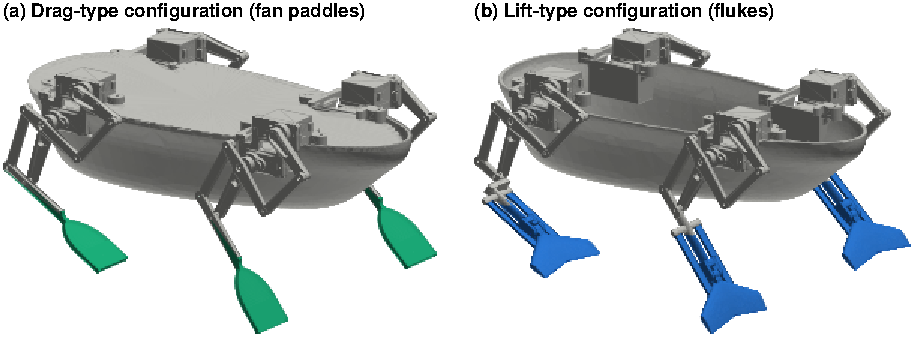
\includegraphics[width=\textwidth]{fig_robot}
  \caption[BODY2 with fan paddles and with flukes]{BODY2 in its two swimming configurations, rendered from the
    CAD models. (a) Drag-type configuration with the folding fan paddles (green) used for walking and
    paddling. (b) Lift-type configuration with a fluke (blue) on a straight foot rod at each leg.}
  \label{fig:robot}
\end{figure}

\section{Propulsors}
\label{sec:plat-propulsors}

\Cref{fig:propulsors} and \cref{tab:propulsors} summarize the two propulsors.

\paragraph{Drag-type: folding fan paddle.} The foot is a \SI{120}{\degree} fan of radius
\SI{42}{\milli\metre} at the end of a \SI{50}{\milli\metre} rod; \emph{fan} denotes the folding blade alone and \emph{paddle} the
blade on its rod. Open, the fan has an area of
\SI{18.5}{\square\centi\metre} (\SI{20.5}{\square\centi\metre} including the rod). A cable folds it for the
recovery stroke. In the current hardware the folded fan is still \SI{30}{\milli\metre} wide
(\SI{12.5}{\square\centi\metre}, 68\,\% of the open area), which makes the spatial asymmetry weak. A folded
width of \SI{12}{\milli\metre} (\SI{5.9}{\square\centi\metre}) is assumed for the optimized stroke in
\cref{sec:res-drag}. The fan is always oriented normal to the stroke; its opening and closing are treated as
instantaneous switches between two rigid shapes (\cref{sec:cfd-composite}).

\paragraph{Lift-type: fluke.} The fluke (design ``A2'') is a small swept foil with a span of
\SI{60}{\milli\metre}, a root chord of \SI{34}{\milli\metre}, a planform area of \SI{11.2}{\square\centi\metre}
and an aspect ratio of about 3.2. Its section is a thick symmetric profile similar to NACA\,0021. It is mounted
on a pin near its leading edge at the lower end of a straight foot rod, so that it can pitch about a spanwise
axis. On the hardware the pitch is passive, set by the hydrodynamic moment against a leaf spring and two end
stops. In the simulations of this thesis the pitch angle $\theta(t)$ is prescribed; how closely a passive
fluke follows a prescribed schedule is not studied here.

\begin{figure}[t]
  \centering
  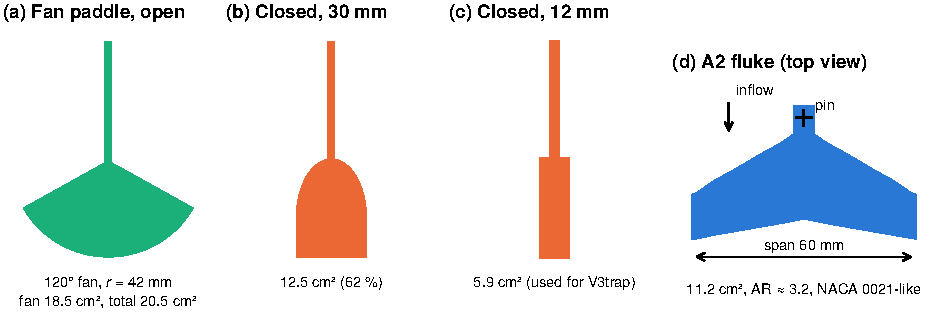
\includegraphics[width=\textwidth]{fig_propulsors}
  \caption[Propulsor geometries]{Propulsor geometries used in the CFD, drawn to scale. (a) Open fan paddle.
    (b) Folded fan of the current hardware, \SI{30}{\milli\metre} wide. (c) Folded fan of
    \SI{12}{\milli\metre} width assumed for the optimized stroke. (d) Fluke A2 in top view, with its pin
    axis.}
  \label{fig:propulsors}
\end{figure}

\begin{table}[t]
  \centering
  \caption[Propulsor data]{Propulsor data. Areas are planform areas of the propulsor without the linkage.}
  \label{tab:propulsors}
  \small
  \begin{tabularx}{\textwidth}{@{}l>{\raggedright\arraybackslash}X>{\raggedright\arraybackslash}X@{}}
    \toprule
    & Fan paddle (drag type) & Fluke A2 (lift type) \\
    \midrule
    Shape & \SI{120}{\degree} fan, $r=\SI{42}{\milli\metre}$, on \SI{50}{\milli\metre} rod & swept foil, NACA\,0021-like \\
    Area & \SI{18.5}{\square\centi\metre} open; \SI{12.5}{} or \SI{5.9}{\square\centi\metre} folded (30 or 12\,mm wide) & \SI{11.2}{\square\centi\metre} \\
    Size & fan radius \SI{42}{\milli\metre} & chord \SI{34}{\milli\metre}, span \SI{60}{\milli\metre} \\
    Principle & drag, folding recovery & lift, pitching about pin \\
    Degrees of freedom & $\psi,\phi$ + open/closed & $\psi,\phi$ + pitch $\theta$ \\
    Frequency & \SI{0.8}{\hertz} (robot gait), \SI{1.39}{\hertz} (V3trap) & \SI{2}{\hertz} \\
    \bottomrule
  \end{tabularx}
\end{table}

\section{Leg Motions}
\label{sec:plat-motions}

\Cref{fig:kinematics} shows the motions studied.

\paragraph{Robot gait.} The robot currently swims with a gait taken from video of the robot: period
\SI{1.25}{\second}, $\mathrm{DUTY}=0.5$, a sinusoidal hip sweep of \SI{60}{\degree} and the fan folded to
\SI{30}{\milli\metre} during the recovery. It was designed for walking and serves as the baseline.

\paragraph{Optimized drag-type stroke (V3trap).} The stroke derived in \cref{sec:res-drag} has a period of
\SI{0.72}{\second} and $\mathrm{DUTY}=0.382$. The hip sweeps \SI{50}{\degree} centred on the vertical
(\SIrange{120}{70}{\degree}), so that the paddle moves nearly straight backwards and stays normal to its path.
The hip velocity follows a trapezoidal law with ramps of about \SI{45}{\milli\second}. During the recovery the
parallelogram curls the paddle upwards and the fan is folded to \SI{12}{\milli\metre}. The fan is closed at
$\tau_c=0.33$, the start of the power-stroke deceleration, and opened at $\tau_o=0$, the reversal point at the
end of the recovery (\cref{fig:kinematics}a).

\paragraph{Fluke motion.} The fluke leg keeps the hip fixed and swings the foot rod about the knee, so that
the fluke's pin moves up and down on a flat arc: $\pm\SI{24.9}{\degree}$ at \SI{2}{\hertz}, a vertical stroke
of \SI{39.2}{\milli\metre} and a peak heave speed of about \SI{0.28}{\metre\per\second}
(\cref{fig:kinematics}b). The reference motion, called L0, is taken from the whole-robot Flare Live model
(\cref{sec:cfd-flare}): the joint angles and the fluke pitch of one leg were recorded while the fluke pitch
was controlled to hold a target angle of attack at \SI{0.223}{\metre\per\second}, and phase-averaged over the
recorded cycles. The resulting 75th percentile of $|\alpha|$ at this speed is \SI{19.9}{\degree}. Three
families are derived from it:
\begin{itemize}
  \item \emph{L2, fixed pitch schedule:} the L0 motion unchanged at
        \SIlist{0;0.08;0.15;0.30}{\metre\per\second}, as a propeller is tested at fixed rotational speed and
        varying advance speed. Since $\gamma$ changes with $\U$ (\cref{eq:gammamax}), the angle of attack is
        large at low speed and small at high speed.
  \item \emph{L1, angle-of-attack law:} a pitch schedule computed from the heave speed to hold a target
        $\alpha$ of \SI{10}{\degree} or \SI{28}{\degree} at \SI{0.223}{\metre\per\second}, and \SI{20}{\degree} at
        \SI{0.40}{\metre\per\second}. These cases use slightly different hinge paths from L0 and are therefore
        not a clean angle-of-attack sweep.
  \item \emph{L3, speed-scheduled pitch:} the L0 hinge path with the pitch
        schedule~\eqref{eq:l3}, $\theta_0=\gamma_\text{max}/2$, at \SIlist{0.30;0.40}{\metre\per\second}
        ($\theta_0=\SI{21.6}{\degree}$ and \SI{17.6}{\degree}).
\end{itemize}

\begin{figure}[t]
  \centering
  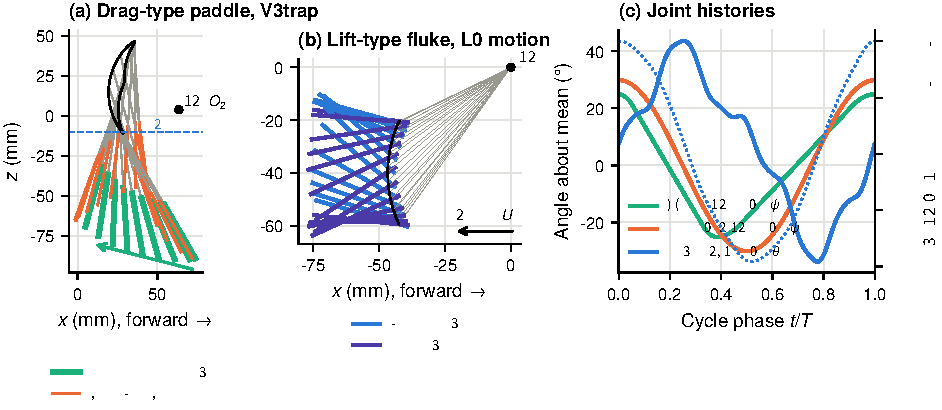
\includegraphics[width=\textwidth]{fig_kinematics}
  \caption[Leg motions]{Leg motions in the hull frame. (a) Optimized drag-type stroke V3trap: paddle positions
    at 25 instants per cycle, open (thick) and closed (thin), and the path of the linkage end point $E$.
    (b) Fluke motion L0: chord positions over one cycle, downstroke and upstroke, with the hinge path. (c) Joint
    histories: hip angle of V3trap and of the robot gait (about their means), fluke pitch angle and hinge
    heave of L0 (dotted, right axis).}
  \label{fig:kinematics}
\end{figure}

Two differences between the propulsors are inherent in this set-up and are kept in mind throughout. First,
the propulsors differ in area (\SI{18.5}{} versus \SI{11.2}{\square\centi\metre}) and in frequency, so thrust
per leg, thrust per area and thrust per power are all reported. Second, the drag-type stroke has been
optimized in several rounds, whereas L0 is a motion taken from another model and was not optimized for
thrust; L3 is the only systematic improvement of the fluke motion. At rest both propulsors draw a similar
hydrodynamic input power of \SIrange{18}{22}{\milli\watt} per leg, so that the comparison is made at a similar
power budget.

\section{Hardware Prototype}
\label{sec:plat-hw}

The lift-type configuration exists as hardware (\cref{fig:hardware}). All four legs carry printed flukes on a passive pin with
a leaf spring. The firmware drives each leg through seven control points per cycle: the thigh is held fixed, the foot bar swings
by $\pm\SI{25}{\degree}$ about the horizontal, and the legs are coordinated in a trot. At \SI{2}{\hertz} this is close to the L0
motion: the pin travels \SI{38.0}{\milli\metre} vertically (L0: \SI{39.2}{\milli\metre}) at a mean heave speed of about
\SI{0.15}{\metre\per\second} (L0: \SI{0.157}{\metre\per\second}), but its peak heave speed is about 15\,\% lower, because the
control points are joined by straight segments. Unlike in the simulations, the hull is mounted reversed, so the robot swims with its
blunt end first. In the water, BODY2 with flukes swam visibly faster than with its fan paddles and its current gait. A first timed
test is compared with the self-propulsion estimate in \cref{sec:res-hw}. The optimized paddle was not tested, because it requires a
controllable fold and a trapezoidal velocity law that the hardware does not have.

\begin{figure}[t]
  \centering
  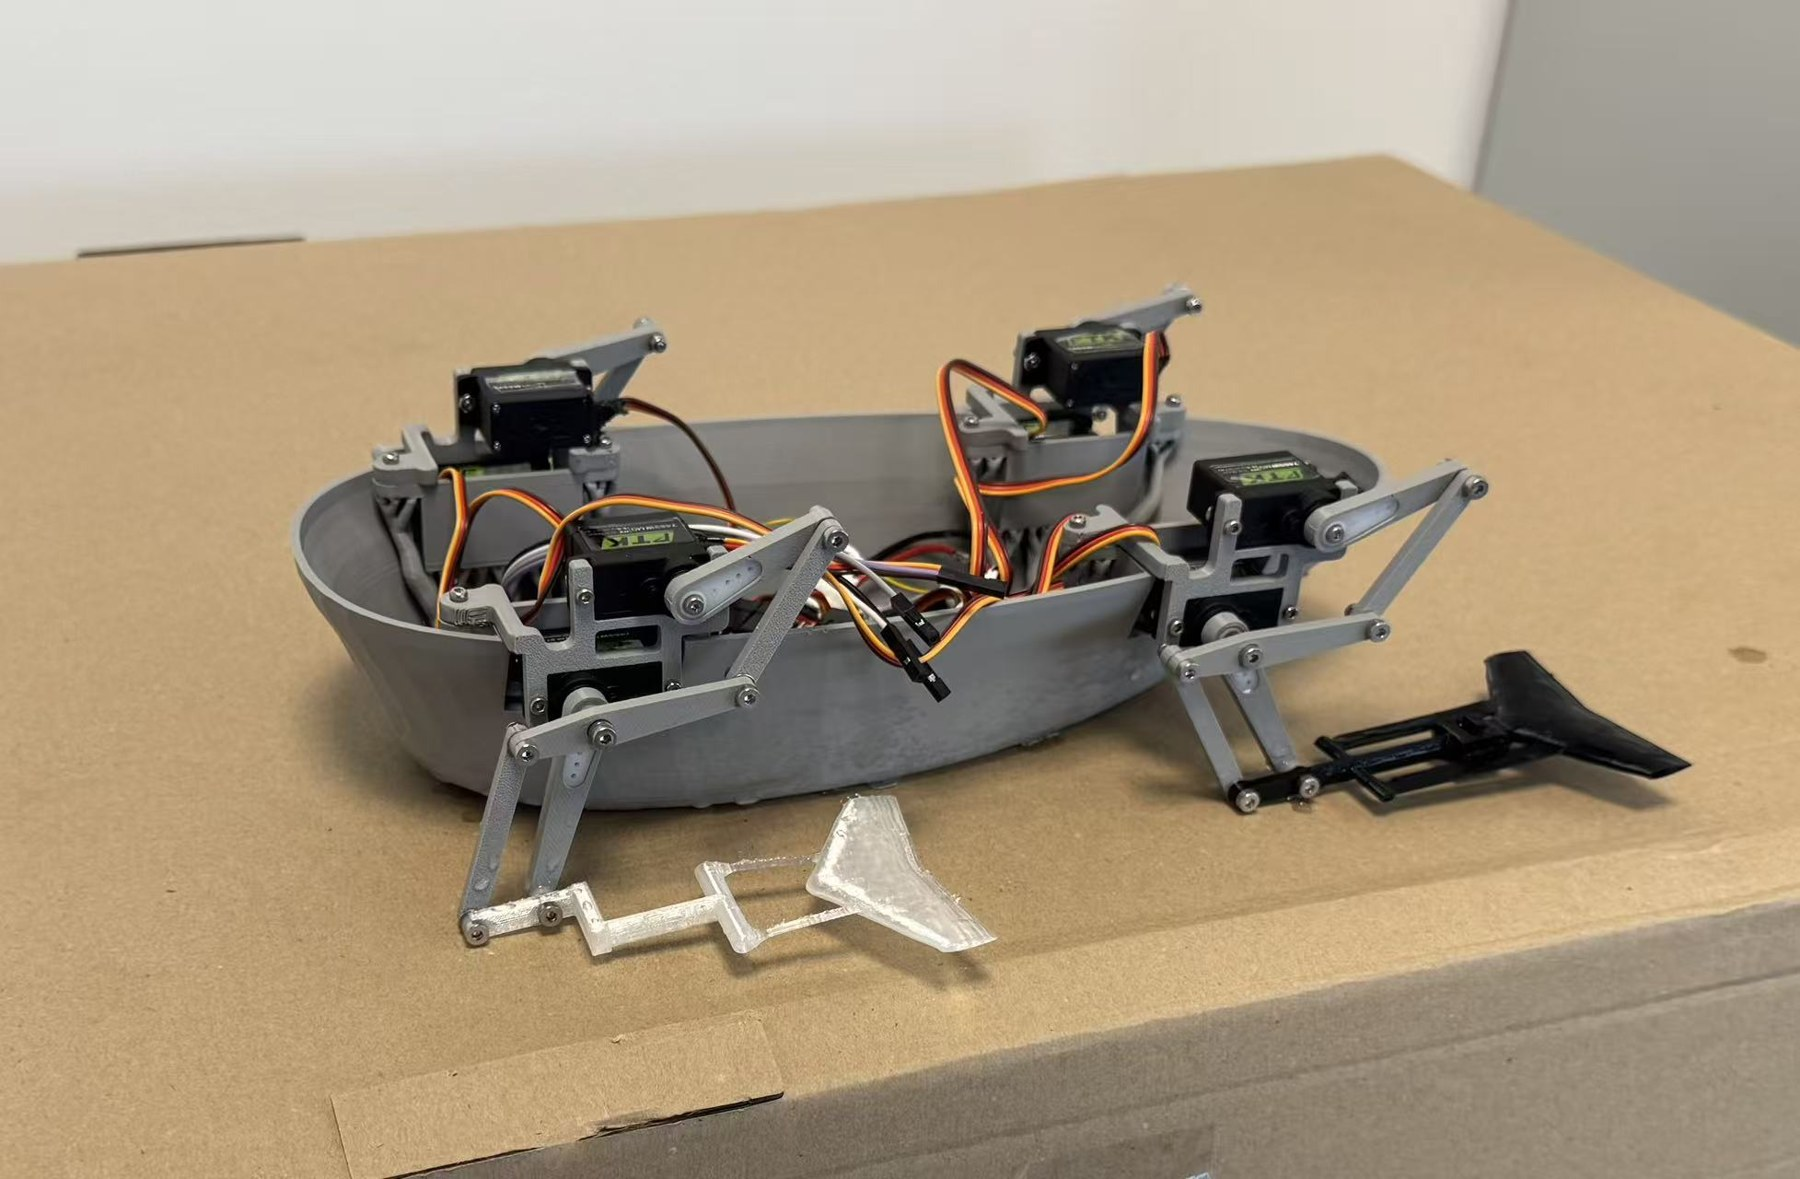
\includegraphics[width=0.78\textwidth]{fig_hardware.jpg}
  \caption[BODY2 hardware with flukes]{Hardware prototype of BODY2 with printed fluke feet mounted on the leg linkages; two of the
    fluke feet are shown resting on the table. Each leg is driven by two PTK\,7465W servos.}
  \label{fig:hardware}
\end{figure}

\chapter{Reduced-Order Gait Optimization}
\label{ch:mujoco}

This chapter addresses RQ1. A whole-robot model with quasi-steady link forces is built in MuJoCo
\cite{Todorov2012}, and its gait is optimized with CMA-ES \cite{Hansen2001,Hansen2016} under actuator and
attitude constraints. The model is cheap enough for thousands of evaluations but its coefficients are not
calibrated. Its purpose is to show which propulsion principle an optimizer selects, and how the answer depends on the physics included, not to predict speeds of BODY2.

\section{Model}
\label{sec:mj-model}

\subsection{Robot}

BODY2 could not be used directly: its CAD-derived model is an open kinematic tree in which the parallelogram
linkages are not closed, and its buoyancy distribution had not been measured. The optimization therefore uses
a simple quadruped model, \texttt{toy\_quad}, of similar size (\cref{fig:mj-model}, \cref{tab:mj-robot}). Each
leg has three hinge joints about the transverse axis: hip, knee and flipper wrist, twelve actuators in total.
The flipper, a thin plate of \qtyproduct{52 x 36}{\milli\metre} whose area of \SI{18.7}{\square\centi\metre} is close to that of the open fan paddle of BODY2, is called \emph{flipper} throughout to distinguish it from the fan paddle and the fluke of
the real robot: it can paddle or flap depending on the physics included, whereas the two propulsors of BODY2 are each built for one
principle. The dry mass is \SI{0.78}{\kilo\gram}; fully submerged, the robot would
displace \SI{1126}{\cubic\centi\metre}, so it floats at the surface like BODY2. The body length of
\SI{0.239}{\metre} is used to express speeds in body lengths per second.

\begin{figure}[t]
  \centering
  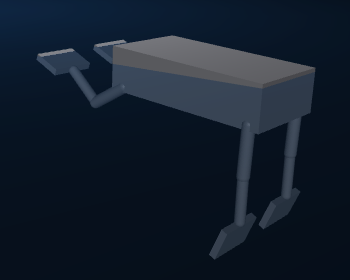
\includegraphics[width=0.42\textwidth]{fig_mj_model.png}
  \caption[MuJoCo model]{The MuJoCo model \texttt{toy\_quad} floating at the surface (rendering from the
    simulation). Each leg has a hip, a knee and a flipper joint.}
  \label{fig:mj-model}
\end{figure}

\begin{table}[t]
  \centering
  \caption[MuJoCo robot model]{The reduced-order robot model \texttt{toy\_quad}.}
  \label{tab:mj-robot}
  \small
  \begin{tabular}{@{}llll@{}}
    \toprule
    Part & Geometry & Size & Mass \\
    \midrule
    Trunk & box & \qtyproduct{0.20 x 0.10 x 0.05}{\metre} & \SI{0.600}{\kilo\gram} \\
    Upper leg ($\times4$) & capsule & $r=\SI{7}{\milli\metre}$, $l=\SI{55}{\milli\metre}$ & \SI{0.020}{\kilo\gram} \\
    Lower leg ($\times4$) & capsule & $r=\SI{6}{\milli\metre}$, $l=\SI{50}{\milli\metre}$ & \SI{0.015}{\kilo\gram} \\
    Flipper ($\times4$) & plate & \qtyproduct{8 x 52 x 36}{\milli\metre} & \SI{0.010}{\kilo\gram} \\
    \midrule
    \multicolumn{4}{@{}l}{Joint ranges: hip and knee $\pm\SI{1.3}{\radian}$, flipper $\pm\SI{1.6}{\radian}$;
      legs at $\pm\SI{0.085}{\metre}$ fore--aft, $\pm\SI{0.045}{\metre}$ lateral} \\
    \multicolumn{4}{@{}l}{Dry mass \SI{0.78}{\kilo\gram}; added mass \SI{0.28}{\kilo\gram}; body length
      \SI{0.239}{\metre}; time step \SI{2}{\milli\second}, implicit integrator} \\
    \bottomrule
  \end{tabular}
\end{table}

\subsection{Hydrodynamic Forces}

Each geometric body $k$ receives a quasi-steady force, scaled by its immersed fraction $f_k$ and applied at its
centre:
\begin{equation}
  \bm F_k = \rho g V_k f_k\,\bm e_z
  \;-\; \tfrac12\rho f_k \sum_{i=1}^{3} C_{D,i} A_i\, v_i|v_i|\,\bm e_i
  \;-\; c_v f_k\,\bm v \;+\; \bm L_k .
  \label{eq:mj-force}
\end{equation}
Here $\bm v$ is the velocity of the body centre relative to still water, $v_i$ its components along the
body axes $\bm e_i$, and $A_i$ the projected areas; $c_v$ is a small linear damping coefficient (0.05, 0.02 and \SI{0.10}{\newton\second\per\metre} for flipper, links and trunk) that matters only at very low speed. The drag is anisotropic: the flipper has
$C_D=(2.2,\,0.10,\,0.10)$ normal to and along its faces, the links $(0.5,0.5,0.25)$ and the trunk
$(0.9,1.6,1.8)$. This anisotropy is the only source of thrust in a drag-only model. The immersed fraction is
computed from the actual vertical extent of each body, so a flipper that breaks the surface loses its force.
Added mass $m_a=C_a\rho V$ ($C_a=1.0$ for the flipper, 0.3 for the links, 0.2 for the trunk) is added to the
body inertia together with a constant upward force $m_a g$ that cancels its weight. This isotropic
approximation is unconditionally stable, unlike an explicit $\dot{\bm v}$ term. The coefficients are
literature values of the same level as in beaver-robot models \cite{Chen2021,Chen2022}; they are not
calibrated.

\paragraph{Lift.} All terms of \eqref{eq:mj-force} except $\bm L_k$ oppose some component of the relative flow.
An optional post-stall flat-plate lift acts on the flippers,
\begin{equation}
  C_L(\alpha) = c_l \sin 2\alpha, \qquad |\bm L| = \tfrac12\rho\,C_L\,A_\text{face}|\bm v|^2 f,
  \label{eq:mj-lift}
\end{equation}
normal to $\bm v$ in the plane spanned by $\bm v$ and the plate normal, where $\alpha$ is the angle between
$\bm v$ and the plate. The value $c_l=1.1$ is a textbook flat-plate value without an aspect-ratio correction.
At small $\alpha$ the lift grows like $\alpha$ and the drag like $\alpha^2$, so a fast, shallow, feathered
stroke produces almost no thrust in the drag-only model but a large thrust with lift. With the lift switched
off, a lift-based gait cannot win, because the mechanism that would make it win is absent.

\paragraph{Thrust decomposition.} To identify the mechanism of a gait, the signed impulses of the lift terms and
of the drag terms (including the linear term) along the swimming direction are accumulated over the scoring
window. A gait with positive lift impulse and negative drag impulse is \emph{lift-propelled}: lift supplies the
forward impulse, and drag only opposes it. The decomposition was checked with a coasting test, in which the
initial momentum equals the sum of the impulses. To quantify how much of the propulsion lift provides, the
\emph{lift thrust share}
\begin{equation}
  s_L = \frac{I_L}{|I_\text{trunk}|}
  \label{eq:liftshare}
\end{equation}
relates the forward impulse $I_L$ of the lift terms to the drag impulse of the trunk; the drag on the limbs is
accumulated separately. A paddling stroke has $s_L\approx0$; a lift-propelled stroke has $s_L>1$, because lift must also
overcome the drag of the limbs themselves. The share can be imposed as a further limit, $s_L\le s_\text{max}$, which forces
drag-based strokes in a model that contains lift (\cref{sec:mj-liftshare}).

\subsection{Servo Model}
\label{sec:mj-servo}

The actuators are position servos with a stiffness of \SI{60}{\newton\metre\per\radian} and critical damping. Real hobby servos cannot move
arbitrarily fast. Each actuator is therefore given the torque--speed characteristic of a DC motor,
\begin{equation}
  \tau = \tau_s\,u - \frac{\tau_s}{\omega_\text{max}}\,\omega, \qquad |u|\le1,
  \label{eq:servo}
\end{equation}
with stall torque $\tau_s=\SI{3}{\newton\metre}$ and no-load speed
$\omega_\text{max}=\SI{400}{\degree\per\second}$. These values were chosen before the servos of BODY2 were identified; the PTK\,7465W has a lower stall torque and a higher no-load speed (\cref{sec:plat-robot}), and the consequences are discussed in \cref{sec:disc-limits}. The back-EMF term is a viscous damping
$b=\tau_s/\omega_\text{max}\approx\SI{0.43}{\newton\metre\second\per\radian}$, which is added to the joint
damping and integrated implicitly by MuJoCo; the result is independent of the time step. Two simpler
variants failed: limiting only the rate of the command let the legs be dragged back and then snap forward at
\SI{1500}{\degree\per\second}, and rewriting the torque limit at every step acted as an explicit damping that
oscillated at up to \SI{3000}{\degree\per\second} and changed the result six-fold with the time step.

Two power measures are reported. The optimization uses the mean mechanical power at the motor shafts,
$\sum_j\langle|\tau_{m,j}\,\omega_j|\rangle$ with the motor torque $\tau_m=\tau-b\,\omega$ and no recovery of
braking energy. The electrical power adds the copper loss of the same motor model,
$\sum_j\langle\max(\tau_{m,j}\omega_j,0)+\tau_{m,j}^2\,\omega_\text{max}/\tau_s\rangle$, which follows from
\eqref{eq:servo} without new parameters; it is computed after the optimization and used as a check. The cost of
transport in this chapter is power over speed in \si{\joule\per\metre}.

\section{Gait Parametrization}
\label{sec:mj-gait}

Every actuator $i$ follows the target angle
\begin{equation}
  q_i(t) = q_{0,i} + r(t)\sum_{h=1}^{H} A_{i,h}\,\sin\!\big(h\,\vartheta(t)+\varphi_{i,h}\big), \qquad H=2,
  \label{eq:gait}
\end{equation}
with offset $q_{0,i}$, amplitudes $A_{i,h}$, phases $\varphi_{i,h}$ and a ramp $r(t)$ from 0 to 1 over the
first \SI{1.5}{\second}. The duty warp $\vartheta(t)$ lets the power stroke be faster or slower than the recovery
while keeping the period: with the cycle progress $c=(ft)\bmod1$,
\begin{equation}
  \vartheta = \begin{cases}
    \pi\,c/\mathrm{DUTY}, & c<\mathrm{DUTY},\\
    \pi + \pi\,(c-\mathrm{DUTY})/(1-\mathrm{DUTY}), & c\ge\mathrm{DUTY}.
  \end{cases}
  \label{eq:duty-warp}
\end{equation}
The second harmonic, which is invariant under a phase shift of $\pi$, can express the feathering of the
flipper. It is not necessary for net thrust: a single harmonic already propels the model. Joints of the same
type share amplitude and offset. The search ranges are $f\in[0.2,2.5]$\,Hz, $\mathrm{DUTY}\in[0.25,0.75]$,
$A\in[0,0.9]$\,rad and $q_0\in[-0.5,0.5]$\,rad, normalized to $[0,1]$.

The coordination of the legs is either free, with an independent phase for every actuator (35 parameters),
or fixed to a \emph{gait family} with one phase per joint type (17 parameters). The families are defined by
the delay of each leg relative to the left fore leg FL, applied in time before the duty warp:
\begin{center}
  \small
  \begin{tabular}{@{}lll@{}}
    \toprule
    Family & Common name & Delays of FR, BL, BR (fraction of period) \\
    \midrule
    \texttt{diag} & trot & 0.5, 0.5, 0 \\
    \texttt{lr} & pace & 0.5, 0, 0.5 \\
    \texttt{fb} & bound & 0, 0.5, 0.5 \\
    \texttt{wave} & walk & 0.5, 0.75, 0.25 \\
    \texttt{inphase} & pronk & 0, 0, 0 \\
    \bottomrule
  \end{tabular}
\end{center}
To classify a free gait, the delays of the joint type with the largest first-harmonic amplitude are compared
with each family, and the family with the smallest mean circular distance is reported together with that
distance (0 = identical, 0.5 = opposite).

\section{Objective, Constraints and Optimizer}
\label{sec:mj-objective}

Each evaluation settles the robot for \SI{1.0}{\second}, ramps the gait in over \SI{1.5}{\second} and scores the
following \SI{8}{\second}, rounded up to whole stroke periods. The speed is the displacement along the initial
heading divided by the window length, so turning is penalized automatically. Two objectives are used: the
highest speed, or the lowest mean mechanical power subject to a minimum speed $v_\text{min}$. All settings are listed in \cref{tab:app-mujoco}.

Stability is imposed by limits, not by weights. With RMS values of heading error, roll and pitch and their
limits $\ell_k$, the penalty is
\begin{equation}
  p = \sum_k \frac{\max(0,\mathrm{RMS}_k-\ell_k)}{\ell_k}
    \;\big[+\,\text{surfacing and } v_\text{min} \text{ terms}\big], \qquad
  \text{fitness} = \begin{cases} \text{objective}, & p=0,\\ -1000-p, & p>0. \end{cases}
  \label{eq:feasibility}
\end{equation}
Any infeasible gait thus scores below every feasible one; speed cannot buy back a violation. An earlier
additive weighting of speed and attitude failed once the legs could move freely: speed dominated, and the best
gait rolled by \SI{42}{\degree} and yawed by \SI{44}{\degree}. Two limit sets are used: a moderate one,
heading/roll/pitch $10/10/\SI{15}{\degree}$, used in this chapter, and a strict one, $10/5/\SI{5}{\degree}$, used for the
coordination study in \cref{app:coord}. Where stated, the
fraction of time in which any limb is less than half immersed (surfacing) is limited to 5\,\%, because the
model has no free-surface physics.

The optimizer is CMA-ES with population 16 and initial step size 0.25 in the normalized space, run for 2500
evaluations unless stated otherwise, with several seeds per condition. Each result is a bound of what the model
allows: a lower bound for the highest speed and an upper bound for the least power. Values are given as mean
$\pm$ standard deviation over seeds.

\section{Results}
\label{sec:mj-results}

\subsection{Baseline and Servo Limit}

A hand-designed trot at \SI{1.2}{\hertz} swims at \SI{0.070}{\metre\per\second} (0.29 body lengths per second)
with \SI{26.7}{\degree} RMS pitch and servos saturated 85\,\% of the time. Without the servo model, the
optimizer found gaits with joint speeds of \SIrange{2700}{4200}{\degree\per\second}, about seven to ten times the servo limit. Replayed with the servo model, the best of them did not move forward
(\SI{-0.001}{\metre\per\second}). Re-optimized with the servo model, three free-phase searches reached
\SIrange{0.11}{0.25}{\metre\per\second}, all close to a bound. The servo limit therefore has to be part of the
model; all following results include it.

\subsection{Drag versus Lift at Equal Speed}

Comparing the fastest gaits of the two physics would be unfair, because power rises steeply with speed and the
fastest gaits differ in speed. The comparison is therefore made at equal speed: the least mechanical power
needed to reach $v_\text{min}\in\{0.10,0.20,0.30\}$\,m/s under moderate limits and at most 5\,\% surfacing,
over five families and two seeds (\cref{tab:mj-pareto}, \cref{fig:mj-pareto}).

\begin{table}[t]
  \centering
  \caption[Least power at equal speed, drag versus lift]{Least mean mechanical power to reach a required speed,
    moderate limits, best over five families and two seeds (family of the best solution and number of feasible searches out of
    ten in brackets). Left: drag-based strokes in a model without lift; middle: drag-based strokes forced by $s_L\le0.1$ in the
    model with lift (\cref{sec:mj-liftshare}); right: unconstrained strokes in the model with lift.}
  \label{tab:mj-pareto}
  \small
  \begin{tabular}{@{}cccc@{}}
    \toprule
    Required speed & Drag-only model & Lift model, $s_L\le0.1$ & Lift model, free \\
    \midrule
    \SI{0.10}{\metre\per\second} & \SI{0.23}{\watt} (walk) & \SI{0.42}{\watt} (bound; 2/10) & \SI{0.10}{\watt} (bound; 10/10) \\
    \SI{0.20}{\metre\per\second} & \SI{1.04}{\watt} (bound) & \SI{5.50}{\watt} (pronk; 1/10) & \SI{0.55}{\watt} (pronk; 8/10) \\
    \SI{0.30}{\metre\per\second} & \SI{3.10}{\watt} (trot) & none (0/10) & \SI{0.97}{\watt} (bound; 4/10) \\
    \bottomrule
  \end{tabular}
\end{table}

Three results are robust. First, whenever lift is in the model and not suppressed, every feasible optimum is
lift-propelled: in all 22 feasible lift optima of this experiment the lift impulse is positive
(\SIrange{0.46}{2.2}{\newton\second} on the front) and the drag impulse negative. The optimizer never paddles when it can
flap. Second, at equal speed
the lift-propelled gaits need about one half to one third of the power of the best drag-only gaits, at all three
speeds. Third, each optimum depends on its physics: with lift removed, the lift optima keep only 35--58\,\% of
their speed, and 26 of the 27 drag optima no longer satisfy the attitude limits when lift is added, because lift also
creates moments on the trunk (\cref{sec:mj-liftshare}). The size of the ratio is not reliable: the searches have not converged (a second seed lowered the
drag-only power at \SI{0.20}{\metre\per\second} from 2.99 to \SI{1.04}{\watt}), so both fronts are upper bounds. The ranking is the same with the electrical power, which includes the copper losses of the servos: the drag-only front needs 0.22, 1.14 and \SI{2.80}{\watt}, the lift front 0.10, 0.47 and \SI{0.86}{\watt}.

\begin{figure}[t]
  \centering
  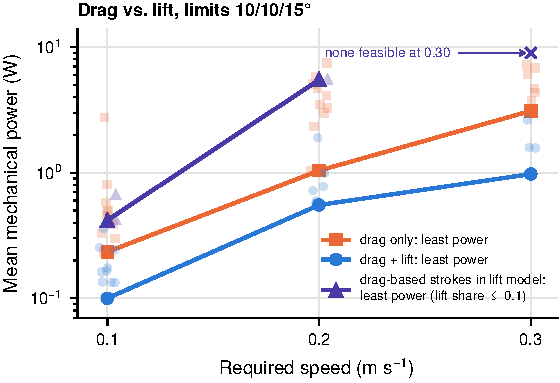
\includegraphics[width=0.62\textwidth]{fig_mj_pareto}
  \caption[Least power at equal speed]{Least mechanical power to reach a required speed, moderate limits: drag-only model, model
    with lift, and drag-based strokes forced by $s_L\le0.1$ in the model with lift. Pale markers are the individual optima of each
    family and seed.}
  \label{fig:mj-pareto}
\end{figure}

\subsection{Drag-Based Strokes within the Lift Model}
\label{sec:mj-liftshare}

The comparison of \cref{tab:mj-pareto} between the drag-only model and the lift model is a comparison of two models as
much as of two propulsion principles. A direct test of RQ1 compares both principles within one model. For this, the
least-power searches of the lift model were repeated with the additional limit $s_L\le0.1$ from \eqref{eq:liftshare}, which
admits only strokes that obtain their thrust from drag, with the same speeds, limits, families and seeds as the unconstrained
searches (30 searches).

The results are shown in the middle column of \cref{tab:mj-pareto} and in \cref{fig:mj-pareto}. Only 3 of the 30 searches
found a feasible drag-based stroke; most of the others satisfy the share limit but not the required speed. On this small basis,
the drag-based strokes need 4.2 times the power of the lift-propelled ones at \SI{0.10}{\metre\per\second} (\SI{0.42}{} against
\SI{0.10}{\watt}) and 10 times at \SI{0.20}{\metre\per\second} (\SI{5.50}{} against \SI{0.55}{\watt}), and none reaches
\SI{0.30}{\metre\per\second}, the closest reaching \SI{0.26}{\metre\per\second}. Because the feasible region is narrow, part of the
factor may be due to search difficulty rather than physics; with two seeds and 2500 evaluations, the direction is reliable but the
value is not.

The two comparisons bound the answer. In the drag-only model a paddling stroke does not have to suppress the lift that its
flipper would produce, which favours it; in the lift model it has to, and the constrained search is difficult, which penalizes
it. Together they indicate that in this model a drag-based stroke needs between about two and ten times the power of a
lift-based stroke at the same speed, and that it cannot reach the speed at which lift-propelled gaits still cruise.

A complementary check replays the 27 feasible optima of the drag-only model with lift switched on. For 21 of them the lift
thrust share exceeds 0.1 (median 1.26), so the same leg motions are mainly lift-propelled once lift exists, and 26 no longer
stay straight and level. Whether a stroke is drag-based or lift-based is therefore a property of the physics as much as of the
motion: a flipper that crosses the water at an angle produces lift whether the model includes it or not. Paddling strokes found
in a drag-only model cannot be transferred unchanged to a real flipper.

\section{Summary}
\label{sec:mj-summary}

Within this model the answer to RQ1 is clear in direction. When lift is part of the physics and not suppressed, the optimizer selects lift-propelled strokes in all 101 feasible optima (22 in this chapter, the others in the coordination study of \cref{app:coord}). At equal speed they need one half to one third of the
power of the best strokes of a drag-only model. When drag-based strokes are forced within the lift model, the few that are
feasible (3 of 30 searches) need four to ten times the power of the lift-propelled strokes and do not reach
\SI{0.30}{\metre\per\second}; in this model a drag-based stroke therefore costs at least about twice and up to ten times as much. Whether a stroke is drag- or lift-based depends on the physics:
most paddling strokes of the drag-only model become lift-propelled when lift is added. Which coordination of the legs is best
is a separate question, which depends mainly on the attitude limits; it is reported in \cref{app:coord}. Three caveats limit these statements to the model: the coefficients and the lift
slope are not calibrated, the flat-plate lift has no aspect-ratio correction although the flipper has
$\mathit{AR}\approx1.4$, and the searches are not fully converged, particularly the constrained search for drag-based strokes. \Cref{ch:cfd,ch:results} therefore test the
central claim, that lift-based flapping beats drag-based paddling, with resolved flow simulations of the real leg.

\chapter{Flow Simulation Methods}
\label{ch:cfd}

Two flow solvers are used. Single-leg simulations with OpenFOAM resolve the flow around one propulsor and
provide the thrust and power data of \cref{ch:results}. Whole-robot simulations with the real-time
lattice-Boltzmann solver Flare Live provide the reference fluke motion and qualitative trends of the free-swimming robot
(\cref{app:flare-trends}). This chapter describes both.

\section{Single-Leg CFD with Overset Grids}
\label{sec:cfd-of}

\subsection{Governing Equations and Solver}

The flow of water ($\rho=\SI{1000}{\kilo\gram\per\cubic\metre}$, $\nu=\SI{1.0e-6}{\square\metre\per\second}$) is modelled as incompressible, laminar and single-phase. The Reynolds numbers of
$10^3$--$10^4$ (\cref{sec:fund-forces}) lie in the laminar-to-transitional range where the forces are dominated by
the separated vortices at the edges, and no turbulence model is used. The incompressible Navier--Stokes equations
are solved with \texttt{overPimpleDyMFoam} of OpenFOAM v2606 \cite{Weller1998}, a finite-volume solver with the
PIMPLE pressure--velocity coupling and overset (Chimera) grids \cite{Windt2020}. The time step is adapted to a
maximum Courant number of 0.8.

Overset grids are chosen because the propulsors rotate by up to \SI{120}{\degree} relative to the hull per cycle.
A body-fitted component mesh moves rigidly with the propulsor inside a stationary background mesh. In every
time step, background cells covered by the propulsor are removed (hole cutting), and the solutions are coupled by
interpolation at the fringe cells. The inverse-distance stencil is used; for some cases it crashed in the stencil
update, and those cases were continued from their last saved time with the tracking inverse-distance variant. As
a guard against failed hole cutting, the number of hole cells is checked in the first time step and the case is
restarted with another stencil if it exceeds 3\,\% of all cells or is below 50.

\subsection{Domain, Boundary Conditions and Motion}

The simulations are carried out in a frame that moves with the hull. The forward speed $\U$ enters as a uniform
inflow at the upstream boundary; the downstream boundary has a fixed pressure and an inlet--outlet condition for the velocity. The top
of the domain is a slip wall \SI{12}{\centi\metre} above the fluke, a rigid lid that represents deep water without
a free surface; the lateral and bottom boundaries are also slip walls far from the propulsor. The propulsor's
rigid-body motion is prescribed as a table of positions and orientations from the leg kinematics of
\cref{sec:plat-motions}. To avoid pressure spikes and collapsing time steps from an impulsive start, the fluke
motion starts from rest with a smooth step over the first half cycle. Three cycles are simulated; means are taken
over the last two for the fluke and over the third for the fan paddle.

Only the propulsor is simulated: the fluke without its foot rod, and the fan paddle with its thin
\SI{3}{\milli\metre} rod but without the crank and parallelogram. The linkage contributes only drag, which is assumed to be the same for both propulsors and is accounted for in the resistance of the self-propulsion balance
(\cref{sec:res-selfprop}). The rod contributes about 1\,\% of the paddle thrust. The hull resistance used in \cref{sec:res-selfprop} comes from separate two-phase simulations of the bare hull with a free surface, which are not described further here.

\subsection{Meshes}

Both meshes are built with \texttt{snappyHexMesh} from the propulsor surface. For the fluke, a clean CFD geometry
is used: the pin hole and the end-stop arm of the printed part are removed and the \SI{0.1}{\milli\metre}
trailing edge is truncated at 95\,\% chord, because these details produced degenerate cells that reduced the time
step below \SI{e-4}{\second}. The resulting blade deviates from the Flare geometry by a median of
\SI{0.12}{\milli\metre}. The mesh parameters are listed in \cref{tab:meshes}.

\begin{table}[t]
  \centering
  \caption[Mesh parameters]{Mesh parameters of the single-leg simulations. Sizes are the cell edge lengths in the
    refined region around the propulsor.}
  \label{tab:meshes}
  \small
  \begin{tabular}{@{}lccc@{}}
    \toprule
    & Fluke (L cases) & Fan paddle (D cases) & Validation foil \\
    \midrule
    Component mesh (surface) & \SI{1.2}{\milli\metre} (\SI{0.6}{\milli\metre}) & \SI{2.5}{\milli\metre} (\SI{1.25}{\milli\metre}) & \SI{2.5}{\milli\metre} \\
    Background mesh & \SI{2.5}{\milli\metre} & \SI{4}{\milli\metre} & \SI{5}{\milli\metre} \\
    Surface cells per length & $\approx50$ per chord & $\approx34$ per radius & $\approx40$ per chord \\
    Cells, component + backgr. & $1.8\times10^5+5.4\times10^5$ & -- & -- \\
    Cycles simulated / averaged & 3 / 2 & 3 / 1 & 3 / 2 \\
    Start-up & 0.5-cycle smooth step & none & none \\
    \bottomrule
  \end{tabular}
\end{table}

The fan-paddle mesh is coarser than the fluke mesh. It was set up earlier, when the paddle strokes were designed,
and was kept to preserve comparability across the paddle design iterations. Its consequence for the comparison
is discussed in \cref{sec:ver-drag}.

\subsection{Two-State Composite for the Folding Fan}
\label{sec:cfd-composite}

Simulating the folding of the fan would require a deforming geometry. Instead, each paddle stroke is simulated
twice with the same motion: once with the fan open and once with the fan closed. The cycle force history is then
composed from the two runs,
\begin{equation}
  \bm F(\tau) = \begin{cases}
    \bm F_\text{open}(\tau), & \tau_o \le \tau < \tau_c,\\
    \bm F_\text{closed}(\tau), & \text{otherwise},
  \end{cases}
  \label{eq:composite}
\end{equation}
where $\tau$ is the cycle phase and $\tau_o,\tau_c$ are the opening and closing phases (\cref{fig:composite}).
The opening and closing are thus instantaneous, and each run keeps its own wake. The composite is a first-order
model of the folding. Its advantage is that the fold timing can be evaluated after the simulation for any pair
$(\tau_o,\tau_c)$ at no extra cost. It has two systematic errors, both of which make it optimistic.

\paragraph{Neglected change of added mass.} When the fan opens, the water around it must be set in motion; when it
closes, that water is released. In \eqref{eq:composite} the open run starts with a flow that has already been
established while the fan was open, and the closed run ends without having to release anything. With the
water-frame velocity $V$ of the fan (positive forward) and the difference $\Delta m_a$ between the added masses of the
open and the closed fan, the missing impulse on the paddle per cycle lies between two limits:
\begin{equation}
  \Delta J = \begin{cases}
    \Delta m_a\,(V_c - V_o) & \text{potential flow: the released momentum returns to the paddle,}\\
    -\Delta m_a\,V_o & \text{full shedding: the released momentum stays in the wake,}
  \end{cases}
  \label{eq:addedmass}
\end{equation}
where $V_o$ and $V_c$ are the velocities at opening and closing. In a separated flow, part of the released momentum is
shed as a stopping vortex, so the true value lies between the two limits; the opening cost $-\Delta m_a V_o$ has no such
escape and is present in both. The corrected mean thrust is reported as the range
$\Tm+\Delta J/T$ over both limits. The added mass of the open fan was identified from the acceleration phase of the
open-paddle simulation at $\U=0$ by fitting $F_x=-m_a\dot v_x-\tfrac12\rho C_N S\,v_x|v_x|$ to the force history, which gives
$m_a=\SIrange{38}{49}{\gram}$ depending on the fitting window and the reference point, close to the
\SI{38}{\gram} of a disc of the same area. With about \SI{5}{\gram} for the fan folded to \SI{12}{\milli\metre},
$\Delta m_a=\SI{38}{\gram}$ is used for V3trap and \SI{20}{\gram} for the robot gait, whose fan folds only to
\SI{30}{\milli\metre}; the uncertainty of $\Delta m_a$ is about $\pm15$\,\%. When the fan switches while it is at rest in the hull frame, the correction does no work in that frame, and the power $\Pm$ is not corrected. V3trap closes at $\tau_c=0.33$ while the fan still moves; the corresponding work, of order $\tfrac12\Delta m_a V_c^2$ per cycle, is not included in $\Pm$.

Two consequences follow. First, switching at the reversal points of the hip motion, where $V$ equals the forward speed
$\U$, is free of correction at $\U=0$ but costs $\Delta m_a\U$ per cycle at speed. Second, opening the fan before the reversal,
during the deceleration of the recovery, credits the paddle with the momentum that the open fan releases while it
decelerates, without charging it for having set that water in motion. The composite therefore rewards early opening
artificially, and all paddle results in this thesis use $\tau_o=0$.

\paragraph{Wake of the open run.} During the power stroke the open-paddle run moves through the wake of its own open
recovery, which has pushed water forward; the real paddle recovers folded and leaves a much weaker wake. This raises the
relative velocity of the power stroke in the composite. The effect is not quantified and is listed as a limitation.

\begin{figure}[t]
  \centering
  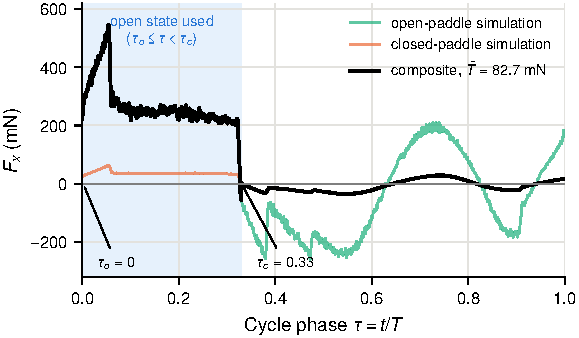
\includegraphics[width=0.62\textwidth]{fig_composite}
  \caption[Two-state composite]{Two-state composite of the fan paddle for V3trap at $\U=0$. The open-paddle
    simulation is used between $\tau_o=0$ and $\tau_c=0.33$ (shaded), the closed-paddle simulation for the rest
    of the cycle. The composite has a cycle-mean thrust of \SI{82.7}{\milli\newton} before the added-mass correction
    of \eqref{eq:addedmass}.}
  \label{fig:composite}
\end{figure}

\subsection{Post-Processing}

Pressure and viscous forces are integrated over the propulsor surface in every time step, and moments are
taken about the hip axis $O_2$. The thrust, the input power and the efficiency follow from
\eqref{eq:thrust}--\eqref{eq:eta}, with the velocity of the fluke's pin or the paddle's reference point and the
angular velocity taken from the motion table. The pitch moment about the fluke pin gives the hinge moment
required from a pitch actuator or spring. The angle of attack is evaluated from \eqref{eq:alpha} with the pin velocity and the pitch angle and is reported either as the 75th percentile of $|\alpha|$ over the cycle, $\alpha_{75}$, or as the
median over the middle part of each half stroke, away from the stroke reversals. For the L1 case with
$\alpha=\SI{10}{\degree}$, whose hinge path had velocity kinks at the seven control points of the trajectory,
the resulting added-mass spikes in the force history were filtered before averaging; this case is marked as
less certain in the results.

\subsection{Case Matrix}

\Cref{tab:cases} lists all single-leg simulations. Each drag-type (D) entry consists of an open and a closed run.

\begin{table}[t]
  \centering
  \caption[Single-leg simulation cases]{Single-leg simulation cases.}
  \label{tab:cases}
  \small
  \begin{tabularx}{\textwidth}{@{}l>{\raggedright\arraybackslash}Xl@{}}
    \toprule
    Case & Description & $\U$ (\si{\metre\per\second}) \\
    \midrule
    L0 & fluke, reference motion from Flare Live & 0.223 \\
    L2 & fluke, L0 motion unchanged (fixed pitch schedule) & 0, 0.08, 0.15, 0.30 \\
    L1 & fluke, angle-of-attack law $\alpha=\SI{10}{\degree}$, \SI{28}{\degree} / \SI{20}{\degree} & 0.223 / 0.40 \\
    L3 & fluke, speed-scheduled pitch $\theta_0=\gamma_\text{max}/2$ & 0.30, 0.40 \\
    L0c & L0 on a coarser mesh (all cell sizes $\times1.33$) & 0.223 \\
    Robot gait & fan paddle, current stroke (30\,mm folded width) & 0, 0.08, 0.15 \\
    V3trap & fan paddle, optimized stroke (12\,mm folded width), $\tau_o=0$, $\tau_c=0.33$ & 0, 0.08, 0.15, 0.223, 0.30 \\
    V & paddle design iterations V1, V2, V3, V3c12, V3c06 (\cref{sec:res-drag}) & 0 \\
    Val & validation: NACA\,0012 heaving and pitching foil (\cref{sec:ver-v1}) & 0.40 \\
    \bottomrule
  \end{tabularx}
\end{table}

The fluke cases took 3--4\,h each and every paddle state about 2.5\,h on eight cores; the validation case, with a
foil of \SI{0.6}{\metre} span, took about 43\,h.

\section{Whole-Robot Simulation in Flare Live}
\label{sec:cfd-flare}

Flare Live \cite{FlareLive} is a commercial solver that couples a lattice-Boltzmann flow solver on adaptive block
grids with a multibody model of the robot and runs close to real time on a GPU. The robot is imported as rigid
bodies connected by joints; each joint is driven by a position controller that follows the commanded trajectory.
The legs and flukes are immersed in the fluid. The hull is not resolved in the fluid; its resistance is applied as
an external force $D=K\,\U|\U|$. Three values of $K$ are used: \SI{3.95}{\newton\second\squared\per\metre\squared}
from the original Flare model, \SI{0.65}{} corresponding to the hull-and-linkage estimate $D_\text{mid}$ of
\cref{sec:res-selfprop} and \SI{0.27}{} corresponding to the bare hull. The model mass is \SI{863}{\gram}, about twice the measured mass of the hardware (\SI{418.8}{\gram}); the difference was not corrected because Flare Live is used only for trends. The
lattice spacing is \SI{3}{\milli\metre}, with a \SI{2}{\milli\metre} lattice as a sensitivity test.

The legs move in a trot at \SI{2}{\hertz} (\SIrange{2}{3}{\hertz} in a frequency sweep). The fluke pitch is actively
controlled by an angle-of-attack law: from the measured heave velocity of the pin and the current swimming speed,
the pitch is set so that \eqref{eq:alpha} gives a target $\alpha$ of \SI{10}{\degree}, \SI{18}{\degree} or
\SI{28}{\degree}, within the fluke's end stops of \SI{-75}{\degree} and \SI{+60}{\degree}.

Two kinds of runs are made:
\begin{itemize}
  \item \emph{Self-propelled runs.} The robot swims freely from rest; speed, power and attitude are averaged over
        the steady part. Power is the mechanical power of the joint drives, and the cost of transport is $P_\text{j}/(mg\U)$ with the joint-drive power $P_\text{j}$.
  \item \emph{Tow runs.} The robot is held fixed in a uniform stream of speed $\U$ with one leg flapping (the L0
        motion) and the others idle. The fluid force on the fluke is obtained from the joint reaction at the pin,
        transformed into the fluke frame, and averaged over $t=\SIrange{3}{9}{\second}$. A run with the fluke idle
        gives the reference drag.
\end{itemize}
The tow runs use exactly the motion of the CFD case L0 and its speed series, so that the fluke force of the two
solvers can be compared directly (\cref{sec:ver-flare}).

\chapter{Verification and Validation}
\label{ch:verification}

The single-leg CFD provides all quantitative statements of \cref{ch:results}. This chapter checks it in three
ways: against a flapping-foil experiment (validation), on a coarser mesh (spatial discretization) and from cycle
to cycle (temporal convergence). It closes with the consequences for the drag-type cases, which were not part of
the mesh study, and with a check of the real-time solver Flare Live against the CFD.

\section{Validation with a Heaving and Pitching Foil}
\label{sec:ver-v1}

\paragraph{Case.} Schouveiler et al.\ \cite{Schouveiler2005} measured the thrust and efficiency of a NACA\,0012
foil in combined heave and pitch in a towing tank, with error bars. One of their points is reproduced with the
same solver, the same overset method and comparable resolution as the fluke cases: chord $c=\SI{0.1}{\metre}$,
span \SI{0.6}{\metre} with free tips, heave amplitude $h_0/c=0.75$, pitch axis at $c/3$, pitch leading heave by
\SI{90}{\degree}, $\mathit{St}=0.25$, maximum angle of attack \SI{15}{\degree}, $\U=\SI{0.4}{\metre\per\second}$
($f=\SI{0.667}{\hertz}$) and $\mathit{Re}=4\times10^4$. The component mesh has \SI{2.5}{\milli\metre} cells
($c/40$), the background \SI{5}{\milli\metre}. Three cycles were simulated without a start-up ramp.

\paragraph{Results.} The streamwise force settles after the first cycle (\cref{fig:verification}a); cycles 2 and 3
differ by less than 0.1\,\%. The simulated motion reaches $\alpha_{75}=\SI{14.6}{\degree}$, consistent with the
prescribed \SI{15}{\degree}, and the mean lateral force is 1.3\,\% of the thrust. The mean thrust is
\SI{1415}{\milli\newton} and the input power \SI{946}{\milli\watt}. \Cref{tab:v1} compares the coefficients
with the experiment.

\begin{table}[t]
  \centering
  \caption[Validation against Schouveiler et al.]{Validation against the experiment of Schouveiler et
    al.\ \cite{Schouveiler2005} (NACA\,0012, $\mathit{St}=0.25$, $\alpha_\text{max}=\SI{15}{\degree}$).}
  \label{tab:v1}
  \small
  \begin{tabular}{@{}lccc@{}}
    \toprule
    & CFD (this work) & Experiment & Deviation \\
    \midrule
    Thrust coefficient $C_T$ & 0.295 & $0.32\pm0.01$ & $-8$\,\% \\
    Froude efficiency $\etaF$ & 0.60 & $0.73\pm0.04$ & $-18$\,\% \\
    \bottomrule
  \end{tabular}
\end{table}

The thrust coefficient is within 8\,\% of the measurement, inside the $\pm$10--15\,\% usually reported for
flapping-foil CFD, and is taken as the main criterion. The efficiency is 18\,\% too low. Three causes act in the
direction observed. (i) The simulated foil has free tips and an aspect ratio of 6, while the experiment was close
to two-dimensional; a finite-wing estimate $\mathit{AR}/(\mathit{AR}+2)=0.75$ suggests tip losses of 10--20\,\%, which
affect efficiency more than thrust because tip vortices cost power. (ii) At $\mathit{Re}=4\times10^4$ the boundary
layer is transitional; a laminar model separates earlier and overestimates the power. (iii) The mesh ($c/40$) is
coarser than in the fluke cases ($c/50$). Because this thesis compares propulsors simulated with the same solver
and settings, such systematic deviations affect both propulsors in the same direction to first order; the tip losses and the laminar separation act mainly on the lift-based fluke, so its advantage is, if anything, underestimated. Absolute efficiencies should be read as conservative.

\begin{figure}[t]
  \centering
  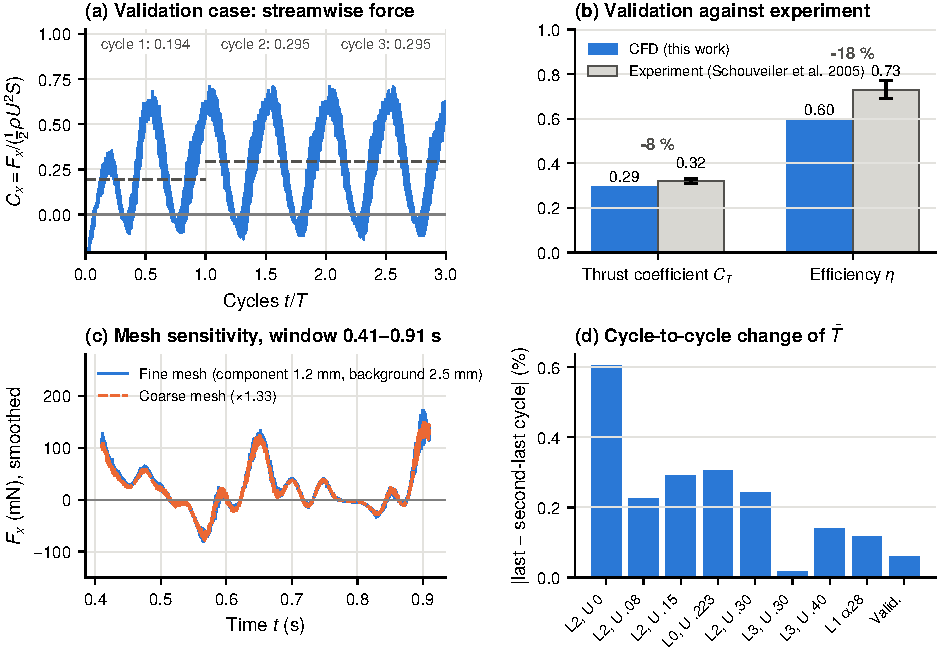
\includegraphics[width=\textwidth]{fig_verification}
  \caption[Verification and validation]{Verification and validation of the single-leg CFD. (a) Validation case:
    streamwise force coefficient with cycle means (dashed). (b) Thrust coefficient and efficiency against the
    experiment of Schouveiler et al.\ \cite{Schouveiler2005}. (c) Fluke L0 on the fine and the coarse mesh over the
    common time window. (d) Change of the mean thrust between the last and the second-last cycle for all fluke cases
    and the validation case.}
  \label{fig:verification}
\end{figure}

\section{Mesh Sensitivity}
\label{sec:ver-mesh}

The reference fluke case L0 was repeated on a mesh in which all cell sizes were multiplied by $r=1.33$ (component
\SI{1.6}{\milli\metre}, background \SI{3.3}{\milli\metre}). The coarse run was stopped at $t=\SI{0.91}{\second}$,
so both runs are compared over the common window $t=\SIrange{0.41}{0.91}{\second}$. The force histories are
nearly identical in shape (\cref{fig:verification}c). The coarse mesh gives 7.3\,\% less thrust
(\SI{19.75}{} versus \SI{21.30}{\milli\newton}), 3.9\,\% less power and 3.4\,\% lower efficiency.

With two meshes the order of convergence cannot be computed. Assuming second order ($p=2$) and a safety factor of
$F_s=1.25$ \cite{Roache1994}, the grid convergence index of the thrust on the fine mesh is
\begin{equation}
  \mathrm{GCI} = F_s\,\frac{|\varepsilon|}{r^p-1} = 1.25\times\frac{0.073}{1.33^2-1} \approx 12\,\%.
  \label{eq:gci}
\end{equation}
The discretization uncertainty of the fluke thrust is therefore taken as about $\pm12$\,\%, and that of power and
efficiency as about $\pm6$\,\%. Since the coarse mesh gives lower thrust, the fine-mesh values are more likely to
be slightly low than high.

\section{Temporal Convergence}
\label{sec:ver-time}

For every fluke case, the mean thrust of the last cycle differs from that of the second-last cycle by at most
0.61\,\% (L2 at $\U=0$), and by at most 0.31\,\% for all other cases (\cref{fig:verification}d). The validation
case differs by less than 0.1\,\%. Averaging over the last two cycles after a half-cycle start-up is therefore
sufficient; the periodic state is reached within the first full cycle. The fan-paddle cases were evaluated in their
third cycle. For the robot gait at \SI{0.08}{\metre\per\second}, cycles 2 and 3 give \SI{7.3}{} and
\SI{5.2}{\milli\newton}; this case, whose thrust is small, has a correspondingly larger uncertainty.

\section{Consequences for the Drag-Type Cases}
\label{sec:ver-drag}

No separate mesh study was run for the fan paddle, and its mesh is coarser than that of the fluke
(\cref{tab:meshes}). Three arguments bound the effect on the conclusions.
\begin{enumerate}
  \item \emph{Flow physics.} The paddle is a thin plate with sharp edges moved broadside. Its separation lines are
        fixed at the edges, whereas the fluke's thrust depends on a leading-edge vortex and leading-edge suction
        that are more sensitive to resolution. The fluke's $\pm12$\,\% is a plausible upper bound for the paddle.
  \item \emph{Low speed.} Up to \SI{0.15}{\metre\per\second} the optimized paddle produces 1.6--2.0 times the thrust
        of the fluke. An error of $\pm12$\,\% does not change this ranking.
  \item \emph{Crossover.} Near the crossover the thrust falls with slopes of about \SI{-110}{} (fluke) and
        \SI{-340}{\milli\newton\second\per\metre} (paddle). A $\pm12$\,\% error of the paddle thrust
        (about \SI{2.5}{\milli\newton}) shifts the crossover by about \SI{0.01}{\metre\per\second}; opposite
        errors of $\pm12$\,\% on both sides shift it by about \SI{0.02}{\metre\per\second}. The uncertainty of the
        added-mass correction (\cref{sec:cfd-composite}) adds less than \SI{0.01}{\metre\per\second}.
\end{enumerate}
The coarser paddle mesh is nevertheless a limitation and is listed in \cref{sec:disc-limits}.

\section{Cross-Check of the Real-Time Solver}
\label{sec:ver-flare}
\label{sec:res-flare}

Flare Live (\cref{sec:cfd-flare}) simulates the whole robot in real time but on a lattice of \SIrange{2}{3}{\milli\metre}. Before
any of its results can be used, its fluke force is checked against the CFD. In the tow runs, the fluke performs exactly the L0 motion of the CFD. Its
angle of attack agrees ($\alpha_{75}=\SI{19.7}{\degree}$ versus \SI{19.9}{\degree} at \SI{0.223}{\metre\per\second}), but its
thrust does not (\cref{fig:flare-fin}). On the \SI{3}{\milli\metre} lattice, Flare Live gives \SI{20.0}{},
\SI{8.5}{} and \SI{-0.1}{\milli\newton} at \SIlist{0;0.1;0.223}{\metre\per\second}, against \SI{45.5}{}, about \SI{34}{} (interpolated) and \SI{21.4}{\milli\newton} in CFD (\cref{tab:app-flare}): 44\,\%, 25\,\% and practically zero. The deficit is about
\SIrange{21}{26}{\milli\newton} at all three speeds, which is the order of the lift-based thrust itself.

The idle fluke, held at its zero position, has a drag of \SI{12.6}{\milli\newton} at \SI{0.223}{\metre\per\second}. At its
incidence of \SI{-25}{\degree} this corresponds to a drag coefficient of about 0.45 based on the planform, a normal value for a
stalled plate. The thrust increment of flapping over idling is \SI{12.5}{\milli\newton}, still well below the CFD thrust.

On a \SI{2}{\milli\metre} lattice the fluke thrust at \SI{0.223}{\metre\per\second} rises to \SI{4.1}{\milli\newton} (19\,\% of
CFD) and the idle drag hardly changes (\SI{11.6}{\milli\newton}). The result is not converged, and a Richardson extrapolation from
the two lattices gives only about \SIrange{8}{12}{\milli\newton}, which indicates that the lattices are far from the asymptotic
range. The cause is resolution: the \SI{34}{\milli\metre} chord spans only 11 cells at \SI{3}{\milli\metre} and 17 at
\SI{2}{\milli\metre}, while the boundary layer at $\mathit{Re}\approx7600$ is about \SI{0.4}{\milli\metre} thick. The leading edge,
where the suction that drives lift-based thrust acts, is not resolved. Resolving it would need a lattice of \SI{1}{\milli\metre}
or finer at many times the cost, which defeats the purpose of a real-time solver.

\begin{figure}[t]
  \centering
  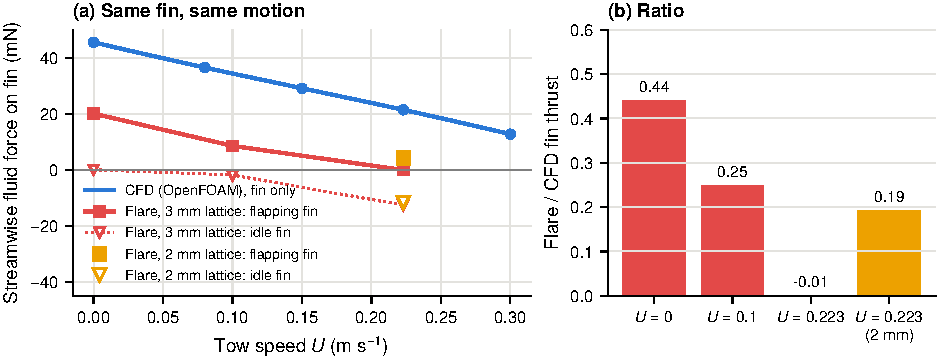
\includegraphics[width=\textwidth]{fig_flare_fin}
  \caption[Flare Live compared with CFD]{Fluke force in Flare Live and in CFD for the same fluke and motion. (a) Streamwise force
    versus tow speed, flapping and idle. (b) Ratio of the Flare to the CFD thrust.}
  \label{fig:flare-fin}
\end{figure}

Flare Live is therefore used only for the reference motion of the fluke and for qualitative trends of the free-swimming
robot, which are collected in \cref{app:flare-trends}; all quantitative statements rest on the CFD.

\section{Summary}
\label{sec:ver-summary}

\Cref{tab:uncertainty} collects the checks of this chapter.

\begin{table}[H]
  \centering
  \caption[Uncertainty summary]{Summary of the verification and validation.}
  \label{tab:uncertainty}
  \small
  \begin{tabularx}{\textwidth}{@{}l>{\raggedright\arraybackslash}X@{}}
    \toprule
    Check & Result \\
    \midrule
    Validation (foil experiment) & $C_T$ $-8$\,\%, $\etaF$ $-18$\,\%; deviations mainly from free tips and laminar model \\
    Mesh sensitivity (fluke) & $\Tm$ $-7.3$\,\% on the $\times1.33$ coarser mesh, GCI $\approx\pm12$\,\% \\
    Temporal convergence & fluke: last two cycles differ by $\le0.61$\,\%; robot gait at \SI{0.08}{\metre\per\second}: 7.3 vs.\ \SI{5.2}{\milli\newton} \\
    Drag-type mesh & not studied; ranking insensitive, crossover within $\pm\SI{0.02}{\metre\per\second}$ \\
    Real-time solver (Flare Live) & fluke thrust 0--44\,\% of CFD on 2--3\,mm lattices; used for trends only \\
    \bottomrule
  \end{tabularx}
\end{table}

The single-leg CFD reproduces the thrust of a flapping foil well and underestimates its efficiency. Its numerical
uncertainty is dominated by spatial discretization, about $\pm12$\,\% in thrust. Differences between propulsors of
less than about 15\,\% are therefore not interpreted as significant in \cref{ch:results}.

\chapter{Results}
\label{ch:results}

This chapter reports the single-leg CFD results and what follows from them for the whole robot. It first
develops the drag-type stroke (\cref{sec:res-drag}) and characterizes the fluke (\cref{sec:res-lift}), then
compares both across speed (\cref{sec:res-compare}), improves the fluke by scheduling its pitch with speed
(\cref{sec:res-l3}), predicts the cruising speed of the robot (\cref{sec:res-selfprop}) and compares it with a first hardware
test (\cref{sec:res-hw}). All forces and powers are
per leg and for the propulsor alone unless stated otherwise.

\section{Design of the Drag-Type Stroke}
\label{sec:res-drag}

The drag-type stroke was optimized at $\U=0$ one factor at a time. The quasi-steady model of \cref{sec:fund-paddle} served as a
surrogate that proposed each change, and CFD evaluated it; the fold timing was then optimized over both switching phases on the
two-state composite. \Cref{tab:drag-design} lists the steps.

\begin{table}[t]
  \centering
  \caption[Design steps of the drag-type stroke]{Design steps of the drag-type stroke at $\U=0$. Each step changes
    one aspect of the previous one. $\Tm$ is the cycle-mean thrust of the two-state composite. All steps before the last
    switch the fan at the reversal points of the hip motion, where the added-mass correction \eqref{eq:addedmass} vanishes
    at $\U=0$; for the last step the range of the correction is given.}
  \label{tab:drag-design}
  \small
  \begin{tabularx}{\textwidth}{@{}l>{\raggedright\arraybackslash}Xcccc@{}}
    \toprule
    Stroke & Change & $T$ (s) & DUTY & $\Tm$ (mN) & $\Pm$ (mW) \\
    \midrule
    Robot gait & baseline, 30\,mm folded, \SI{60}{\degree} sinusoidal sweep & 1.25 & 0.50 & 23.4 & 6.7 \\
    V1 & shorter period, larger thrust & 0.89 & 0.49 & 51.2 & -- \\
    V2 & shorter power stroke & -- & 0.35 & 34.2 & -- \\
    V3 & sweep centred on the vertical (\SIrange{120}{70}{\degree}), slow curl & 0.81 & 0.45 & 49.3 & 16.2 \\
    V3c12 & fan folded to 12\,mm instead of 30\,mm & 0.81 & 0.45 & 56.7 & 13.7 \\
    V3c06 & folded and feathered, 5.6\,mm frontal width & 0.81 & 0.45 & 58.6 & 13.1 \\
    V3trap & V3c12 with trapezoidal velocity law (\SI{45}{\milli\second} ramps) & 0.72 & 0.382 & 75.0 & 20.8 \\
    V3trap, timed & fan closed at the start of the deceleration, $\tau_c=0.33$ & 0.72 & 0.382 & \textbf{73--83} & 21.6 \\
    \bottomrule
  \end{tabularx}
\end{table}

\paragraph{Direction of the stroke.} Centring the sweep on the vertical makes the paddle move nearly straight
backwards with its face normal to the motion. From V1 to V3 the inclination of the power-stroke force from the
swimming direction fell from \SI{19.5}{\degree} to \SI{7.9}{\degree}, and the ratio of mean vertical to mean
horizontal force from 0.52 to 0.28. V2 shows that shortening the power stroke alone loses thrust when the
recovery cannot become correspondingly cheaper.

\paragraph{Folded width.} Folding the fan to \SI{12}{\milli\metre} instead of \SI{30}{\milli\metre} reduced the
recovery drag from \SI{-10.7}{} to \SI{-3.2}{\milli\newton} and raised the mean thrust by 15\,\%. The effective
area ratio $a$, defined as the ratio of the mean force of the closed-only to the open-only run, fell from 0.48 to
0.11. With $a=0.11$, \eqref{eq:duty-opt} gives $x^*=2.2$ and $\mathrm{DUTY}^*=0.69$: the recovery should be much
faster than the power stroke, which the servo speed does not allow. The DUTY of the final stroke, 0.382, was therefore not taken from \eqref{eq:duty-opt} but found in the CFD optimization within the joint speeds that the servos allow (\cref{tab:actuators}). Feathering the folded fan to a frontal width of \SI{5.6}{\milli\metre} added only
3\,\%: the recovery drag is proportional to the width, but at \SI{12}{\milli\metre} it is only about 6\,\% of the
mean thrust. A feathering mechanism is therefore not worthwhile.

\paragraph{Velocity law.} Replacing the cosine hip velocity by a trapezoidal law with \SI{45}{\milli\second} ramps
at the same peak rate and sweep increased the power-stroke impulse by 18\,\%, as predicted by the quasi-steady
$\int v^2\,\mathrm dt$, and the mean thrust by 32\,\%, because the period also shortened from \SI{0.81}{} to
\SI{0.72}{\second}. The price is a higher peak hip moment (\SI{35.6}{} instead of \SI{19.3}{\milli\newton\metre},
$\times1.84$), a higher peak force and 52\,\% more power; the thrust per power fell from \SI{4.1}{} to
\SI{3.6}{\newton\per\watt}. The effective normal-force coefficient of the power stroke in the CFD is 2--3 times the
quasi-steady value and is highest at the start of the stroke, as expected for a starting plate \cite{Kim2011}; it
is the same for both velocity laws.

\paragraph{Fold timing.} The two-state composite (\cref{sec:cfd-composite}) allows the fold timing to be scanned
after the simulation. Without correction, the best pair is $\tau_c=0.33$, $\tau_o=-0.06$ with \SI{87.2}{\milli\newton}. The gain
from opening before the reversal, however, is the artefact described in \cref{sec:cfd-composite}, and the fan is therefore
opened at the reversal, $\tau_o=0$. Closing the fan early, at the start of the power-stroke deceleration ($\tau_c=0.33$,
0.86\,DUTY), raises the uncorrected composite from \SI{75.0}{} to \SI{82.7}{\milli\newton}: the decelerating open fan is no longer
pulled backwards by the water it has set in motion. Whether that water keeps its momentum depends on how much of it is shed as
a stopping vortex, so the added-mass correction \eqref{eq:addedmass} gives a range of \SIrange{73}{83}{\milli\newton}. At rest,
early closing is therefore worth between $-2$ and $+8$\,mN. At forward speed it is never worse and up to \SI{10}{\milli\newton} better, because after $\tau\approx0.33$ the paddle moves backwards more slowly than the oncoming flow and an open fan would only
produce drag; at \SI{0.223}{\metre\per\second}, closing at $\tau_c=0.33$ gives \SIrange{24}{26}{\milli\newton}, against \SIrange{14}{26}{\milli\newton} for closing at the reversal. The final stroke, called V3trap in the rest of this thesis (\cref{fig:composite,fig:kinematics}a),
produces \SIrange{73}{83}{\milli\newton} per leg at rest, 3.1--3.5 times the robot's current gait, at \SI{21.6}{\milli\watt} and
\SIrange{3.4}{3.8}{\newton\per\watt}. These rules agree with those found for crustacean and webbed-foot propulsors: open fully at
the start of the power stroke, close early, keep transitions short \cite{Santos2026,Lin2024}.

\section{The Lift-Type Fluke with a Fixed Pitch Schedule}
\label{sec:res-lift}

\Cref{tab:lift} lists the fluke results with the L0 motion at five speeds. At rest the inflow is purely vertical,
the fluke is stalled ($\alpha_{75}=\SI{73}{\degree}$) and acts as a small paddle; it produces
\SI{45.5}{\milli\newton} at \SI{18.1}{\milli\watt}, about twice the thrust of the robot gait with the fan paddle.
With increasing speed the inflow angle and the angle of attack fall, and the thrust decreases almost linearly, to
\SI{12.7}{\milli\newton} at \SI{0.30}{\metre\per\second}. The input power stays between \SI{15.6}{} and
\SI{18.1}{\milli\watt}. The efficiency rises to a maximum of 0.29 at \SI{0.223}{\metre\per\second}, the speed for
which L0 was designed ($\mathit{St}\approx0.35$ based on the pin excursion, $\alpha_{75}=\SI{19.9}{\degree}$). At
\SI{0.30}{\metre\per\second} the mid-stroke angle of attack drops to about \SI{10}{\degree}, the efficiency falls
to 0.245, and a mean vertical force of \SI{-29}{\milli\newton} appears, more than twice the thrust.

\begin{table}[t]
  \centering
  \caption[Fluke with the L0 motion]{Fluke with the L0 motion (fixed pitch schedule) at different speeds.
    $\mathit{St}$ is based on the peak-to-peak pin excursion of \SI{39.2}{\milli\metre}.}
  \label{tab:lift}
  \small
  \begin{tabular}{@{}lccccc@{}}
    \toprule
    $\U$ (\si{\metre\per\second}) & 0 & 0.08 & 0.15 & 0.223 & 0.30 \\
    \midrule
    $\Tm$ (mN) & 45.5 & 36.5 & 29.1 & 21.4 & 12.7 \\
    $\Pm$ (mW) & 18.1 & 17.1 & 16.6 & 16.3 & 15.6 \\
    $\etaF$ & -- & 0.171 & 0.263 & 0.293 & 0.245 \\
    $\Tm/\Pm$ (\si{\newton\per\watt}) & 2.51 & 2.13 & 1.75 & 1.31 & 0.81 \\
    $\mathit{St}$ & -- & 0.98 & 0.52 & 0.35 & 0.26 \\
    \bottomrule
  \end{tabular}
\end{table}

The wake at \SI{0.223}{\metre\per\second} (\cref{fig:wake}) shows the expected pattern of a thrust-producing
foil: each half stroke sheds a vortex of alternating sign from the trailing edge, and the vortices form a reverse
von K\'arm\'an street that convects downstream.

\begin{figure}[t]
  \centering
  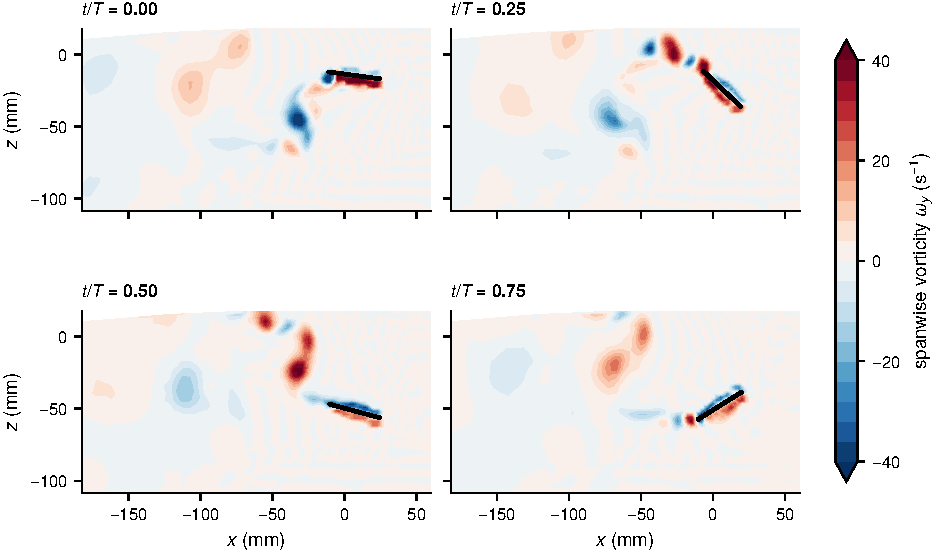
\includegraphics[width=\textwidth]{fig_wake}
  \caption[Wake of the fluke]{Spanwise vorticity in the mid-span plane of the fluke (L0,
    $\U=\SI{0.223}{\metre\per\second}$) at four phases of the third cycle, hull frame; the flow is from right to left
    relative to the fluke. Black line: fluke chord.}
  \label{fig:wake}
\end{figure}

Additional pitch schedules for target angles of attack of \SI{10}{\degree} and \SI{28}{\degree} at \SI{0.223}{\metre\per\second}
produce more thrust than L0 but at lower efficiency (0.20 and 0.24, \cref{tab:app-fluke}); among the cases at this speed the
efficiency is highest for $\alpha_{75}\approx\SI{20}{\degree}$, in line with the efficient range of flapping foils \cite{Read2003}.

\section{Drag versus Lift across Speed}
\label{sec:res-compare}

\Cref{fig:thrust-speed} compares thrust, power and efficiency of the propulsors from rest to
\SI{0.40}{\metre\per\second}; \cref{tab:compare} gives the values.

\begin{figure}[t]
  \centering
  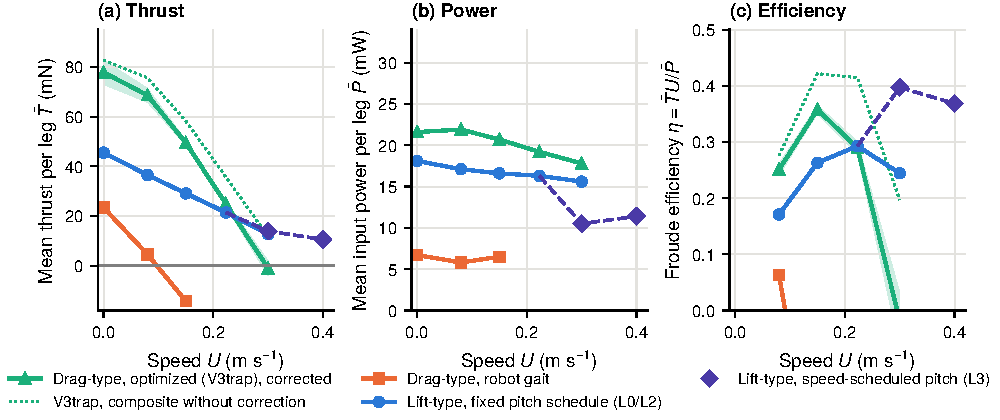
\includegraphics[width=\textwidth]{fig_thrust_speed}
  \caption[Thrust, power and efficiency versus speed]{Single-leg (a) thrust, (b) input power and (c) Froude
    efficiency of the propulsors versus speed. Shaded: range of the added-mass correction of the paddle composites
    \eqref{eq:addedmass}; dotted: V3trap composite without correction.}
  \label{fig:thrust-speed}
\end{figure}

\begin{table}[t]
  \centering
  \caption[Propulsor comparison across speed]{Single-leg thrust $\Tm$ (mN) / input power $\Pm$ (mW) / Froude
    efficiency $\etaF$ across speed. Paddle values include the added-mass correction \eqref{eq:addedmass} as a range; the
    uncorrected composite of V3trap gives 82.7, 75.6, 58.2, 35.7 and \SI{11.7}{\milli\newton}.}
  \label{tab:compare}
  \footnotesize
  \begin{tabular}{@{}ccccc@{}}
    \toprule
    $\U$ (\si{\metre\per\second}) & Paddle, robot gait & Paddle, V3trap & Fluke, fixed (L0/L2) & Fluke, scheduled (L3) \\
    \midrule
    0     & 23.4 / 6.7 / --         & \textbf{73--83} / 21.6 / --                & 45.5 / 18.1 / --      & -- \\
    0.08  & 4--5 / 5.8 / 0.05--0.07 & \textbf{66--71} / 21.9 / 0.24--0.26        & 36.5 / 17.1 / 0.17    & -- \\
    0.15  & $<0$ / 6.5 / --         & \textbf{48--50} / 20.7 / \textbf{0.35--0.37} & 29.1 / 16.6 / 0.26  & -- \\
    0.223 & --                      & 24--26 / 19.2 / 0.28--0.30               & 21.4 / 16.3 / 0.29    & -- \\
    0.30  & --                      & $-4$--2 / 17.8 / $\approx0$                & 12.7 / 15.6 / 0.24    & \textbf{13.9} / 10.5 / \textbf{0.40} \\
    0.40  & --                      & --                                       & --                    & 10.5 / 11.4 / 0.37 \\
    \bottomrule
  \end{tabular}
\end{table}

\paragraph{Low speed.} Up to about \SI{0.15}{\metre\per\second} the optimized paddle is clearly superior. It produces
1.6--2.0 times the thrust of the fluke at 19--28\,\% more power, and at \SI{0.15}{\metre\per\second} it reaches an efficiency of
0.35--0.37, higher than the fluke's maximum of 0.29. Per area there is no difference at rest: the paddle produces
\SIrange{3.9}{4.5}{} and the fluke \SI{4.1}{\milli\newton\per\square\centi\metre}. At \SI{0.223}{\metre\per\second} the fluke
already produces more per area (\SI{1.9}{} versus \SIrange{1.3}{1.4}{\milli\newton\per\square\centi\metre}). The robot gait, in
contrast, loses its thrust almost immediately: at \SI{0.08}{\metre\per\second} only \SIrange{4}{5}{\milli\newton} remain, and at
\SI{0.15}{\metre\per\second} the net force is a drag.

\paragraph{Speed limit of the paddle.} The paddle's thrust falls steeply with speed and vanishes at about
\SI{0.30}{\metre\per\second}. The split into power stroke and recovery (\cref{fig:drag-split}, values in \cref{tab:app-split}) shows why. The power-stroke
thrust of V3trap decreases by 42\,\%, from \SI{88.0}{} to \SI{50.9}{\milli\newton}, because the relative velocity during the power
stroke falls. The recovery drag, however, grows more than sevenfold, from \SI{-5.3}{} to \SI{-39.1}{\milli\newton}, because the
folded paddle and the rod now move forward against the oncoming flow. At speed, opening the fan also costs the momentum
$\Delta m_a\U$ per cycle, \SIrange{12}{16}{\milli\newton} at \SIrange{0.223}{0.30}{\metre\per\second}. At
\SI{0.30}{\metre\per\second} the recovery and the opening together consume the whole power-stroke thrust. For the robot gait, with its
wider folded fan and slower stroke, the recovery drag exceeds the power-stroke thrust already at about
\SI{0.1}{\metre\per\second}. The speed limit of a drag-type paddle on this leg is therefore set by what the paddle has to do outside
the power stroke, not by the speed of the paddle in the power stroke.

\begin{figure}[t]
  \centering
  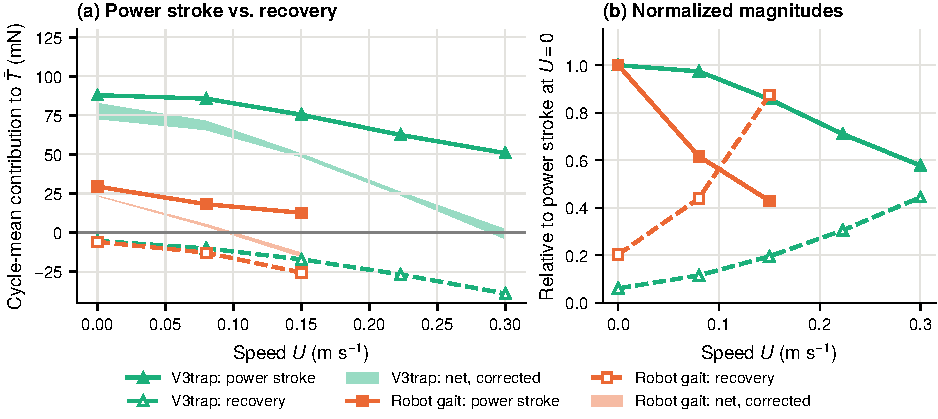
\includegraphics[width=\textwidth]{fig_drag_split}
  \caption[Power stroke and recovery of the paddle]{Contributions of power stroke and recovery to the mean thrust of
    the fan paddle. (a) Absolute values for V3trap and the robot gait; shaded: net thrust including the added-mass correction
    \eqref{eq:addedmass}. (b) Magnitudes relative to the power-stroke thrust at $\U=0$.}
  \label{fig:drag-split}
\end{figure}

\paragraph{Crossover.} The fluke loses thrust more slowly, because it neither recovers against the flow nor changes its shape:
its thrust at \SI{0.30}{\metre\per\second} is 28\,\% of its value at rest, whereas the paddle's is close to zero. Interpolating the
curves, the thrust of the fluke exceeds that of V3trap above \SIrange{0.23}{0.24}{\metre\per\second}, and its efficiency above
\SIrange{0.22}{0.23}{\metre\per\second}. This holds for both pitch schedules, because the speed-scheduled pitch was simulated only at \SIlist{0.30;0.40}{\metre\per\second} and shares the L0 data below. Including the discretization uncertainty of
\cref{sec:ver-drag}, the crossover lies at $0.24\pm\SI{0.02}{\metre\per\second}$ for thrust and at $0.22\pm\SI{0.02}{\metre\per\second}$
for efficiency. Without the added-mass correction, the crossovers would lie at \SI{0.295}{} and \SI{0.285}{\metre\per\second}; the
correction moves them by about \SI{0.06}{\metre\per\second} but does not change their existence.

\section{Speed-Scheduled Fluke Pitch}
\label{sec:res-l3}

With the fixed L0 motion, the fluke's angle of attack falls with speed, which explains its efficiency drop above
\SI{0.223}{\metre\per\second}. The speed-scheduled pitch \eqref{eq:l3} restores the angle of attack
(\cref{fig:l3}). At \SI{0.30}{\metre\per\second} it reduces the pitch amplitude from about \SI{40}{\degree} to
\SI{21.6}{\degree}, and the angle of attack rises accordingly: $\alpha_{75}$ increases from \SI{13.7}{\degree} to \SI{21.0}{\degree}
(\cref{tab:l3,tab:app-fluke}).

\begin{table}[t]
  \centering
  \caption[Speed-scheduled pitch]{Speed-scheduled pitch (L3) compared with the fixed L0 motion (L2). $\bar F_z$: mean vertical
    force; $|M_h|$: peak hinge moment about the pin.}
  \label{tab:l3}
  \small
  \begin{tabular}{@{}lcccccc@{}}
    \toprule
    Case & $\U$ (\si{\metre\per\second}) & $\Tm$ (mN) & $\Pm$ (mW) & $\etaF$ & $\bar F_z$ (mN) & $|M_h|$ (\si{\milli\newton\metre}) \\
    \midrule
    L2, fixed & 0.30 & 12.7 & 15.6 & 0.245 & $-29.4$ & 12.6 \\
    L3, scheduled & 0.30 & \textbf{13.9} & \textbf{10.5} & \textbf{0.398} & $-0.9$ & 7.4 \\
    L3, scheduled & 0.40 & 10.5 & \textbf{11.4} & \textbf{0.368} & $-0.9$ & 7.3 \\
    \bottomrule
  \end{tabular}
\end{table}

At \SI{0.30}{\metre\per\second} the scheduled pitch raises the thrust by 9\,\%, lowers the power by 33\,\% and raises the
efficiency from 0.245 to 0.40, while the paddle produces almost no thrust at this speed. It also removes the mean vertical force
($-29$ to $\SI{-1}{\milli\newton}$), reduces the peak hinge moment by 40\,\% and flattens the force history: the
peak-to-peak streamwise force falls from about \SI{600}{} to \SI{190}{\milli\newton}. At
\SI{0.40}{\metre\per\second} the efficiency is 0.37. Over the three designed speeds the fluke efficiency is 0.29 (L0, 0.223), 0.40 (L3,
0.30) and 0.37 (L3, 0.40), with a maximum near \SI{0.30}{\metre\per\second}. At this speed the Strouhal number based on the pin
excursion is 0.26, inside the range of 0.2--0.4 of efficient cruising in animals and close to the mean value measured for odontocetes \cite{Taylor2003,Rohr2004}; based on the trailing-edge excursion it is somewhat higher. The schedule needs no flow
information, only $\dot h_\text{max}$ and $\U$. On the hardware it corresponds to a pitch amplitude that decreases with speed; how
closely a passive spring can provide it is discussed in \cref{sec:disc-limits-prop}.

\begin{figure}[t]
  \centering
  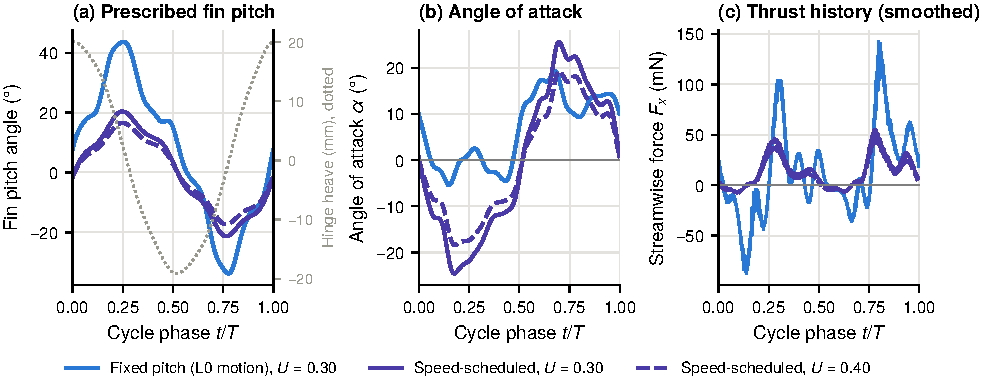
\includegraphics[width=\textwidth]{fig_l3}
  \caption[Speed-scheduled pitch]{Fixed L0 motion versus speed-scheduled pitch. (a) Prescribed fluke pitch (hinge heave
    dotted, right axis). (b) Resulting angle of attack. (c) Streamwise force, smoothed.}
  \label{fig:l3}
\end{figure}

\section{Self-Propulsion Estimate}
\label{sec:res-selfprop}

\paragraph{Resistance.} Three resistance curves bound the resistance of the robot without its propulsors
(\cref{fig:selfprop}a):
\begin{itemize}
  \item $D_\text{low}=\SI{10.8}{\milli\newton}\,(\U/\SI{0.2}{\metre\per\second})^{1.72}$: the bare hull, from separate
        two-phase CFD of the hull at \SIlist{0.1;0.2}{\metre\per\second};
  \item $D_\text{mid}=D_\text{low}+\SI{15.2}{\milli\newton}\,(\U/\SI{0.2}{\metre\per\second})^2$: hull plus the submerged
        linkages, about \SI{26}{\milli\newton} at \SI{0.2}{\metre\per\second}; the linkage term, equivalent to
        $C_DA\approx\SI{7.6}{\square\centi\metre}$, is an engineering estimate, not a measurement; this is the best estimate;
  \item $D_\text{up}=\SI{77.6}{\milli\newton}\,(\U/\SI{0.2}{\metre\per\second})^2$: the whole robot at rest with its fan
        paddles open, from CFD; it counts the paddles' own drag, which is already contained in $\Tm$, and is therefore an
        upper bound.
\end{itemize}
The thrust curves are interpolated with monotone cubic splines and extrapolated linearly beyond the last CFD point.

\begin{figure}[t]
  \centering
  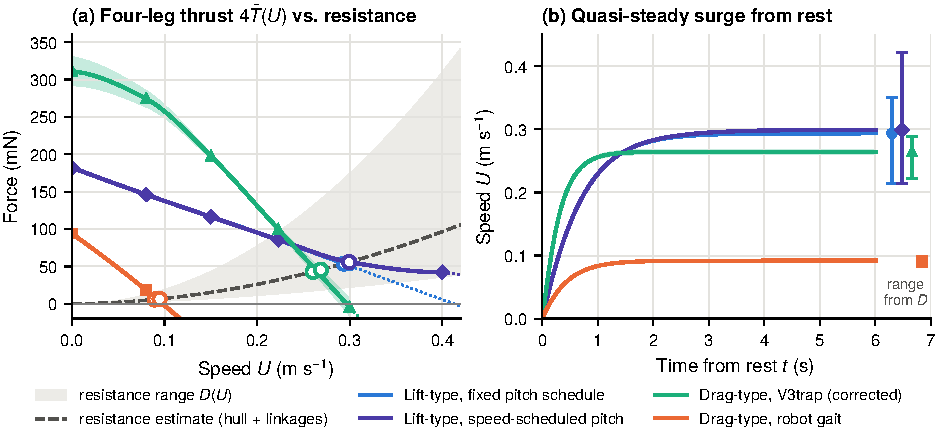
\includegraphics[width=\textwidth]{fig_selfprop}
  \caption[Self-propulsion estimate]{Self-propulsion estimate. (a) Four-leg thrust versus the resistance range; circles mark
    the cruising speeds for $D_\text{mid}$; shaded: range of the added-mass correction of the paddle. Dotted: linear extrapolation. Below \SI{0.30}{\metre\per\second}, where the speed-scheduled pitch was not simulated, its curve uses the fixed-pitch data. (b) Quasi-steady acceleration from rest for $D_\text{mid}$; bars on the right give
    the range of cruising speeds from $D_\text{up}$ to $D_\text{low}$.}
  \label{fig:selfprop}
\end{figure}

\begin{table}[t]
  \centering
  \caption[Predicted cruising speed]{Predicted cruising speed and four-leg input power for $D_\text{mid}$, with the range
    from $D_\text{up}$ to $D_\text{low}$. Paddle values are given as the range of the added-mass correction. $^*$ extrapolated beyond
    the CFD data. $t_{90}$: time to reach 90\,\% of the cruising speed from rest.}
  \label{tab:selfprop}
  \small
  \begin{tabular}{@{}lccccc@{}}
    \toprule
    Propulsor & $\U_c$ (\si{\metre\per\second}) & Range (\si{\metre\per\second}) & $4\Pm$ (mW) & $4\Pm/\U_c$ (\si{\joule\per\metre}) & $t_{90}$ (s) \\
    \midrule
    Drag, robot gait & 0.089--0.095 & 0.082--0.098 & 23.3 & 0.25--0.26 & 0.94--0.99 \\
    Drag, V3trap & 0.260--0.269 & 0.223--0.289 & 73--74 & 0.27--0.28 & 0.67--0.69 \\
    Lift, fixed pitch & 0.294 & 0.214--0.350$^*$ & 62.7 & 0.21 & 1.46 \\
    Lift, scheduled pitch & \textbf{0.299} & 0.214--0.422$^*$ & \textbf{42.0} & \textbf{0.14} & 1.57 \\
    \bottomrule
  \end{tabular}
\end{table}

\paragraph{Cruising speed.} For the best-estimate resistance, the fluke propels the robot at \SI{0.30}{\metre\per\second}, or
1.3 hull lengths per second, and the optimized paddle at \SIrange{0.26}{0.27}{\metre\per\second} (\cref{tab:selfprop}). Both
operating points lie just above the crossover, where the fluke is stronger, but close to it, so the difference in speed is small.
The power differs clearly: the speed-scheduled fluke needs \SI{42}{\milli\watt}, 33\,\% less than the fixed-pitch fluke
(\SI{63}{\milli\watt}) and 43\,\% less than the paddle (\SI{73}{\milli\watt}), which is also slower. The robot's current gait reaches
only about \SI{0.09}{\metre\per\second}. The ranges are wide because the resistance is uncertain, and which propulsor is faster
depends on where the resistance curve crosses the thrust curves. With the high resistance $D_\text{up}$, the operating point
moves below the crossover and the paddle is slightly faster (\SIrange{0.22}{0.23}{} versus \SI{0.21}{\metre\per\second}); with the
low resistance $D_\text{low}$, it moves further above the crossover and the fluke is clearly faster
(\SIrange{0.35}{0.42}{\metre\per\second}, extrapolated, versus \SIrange{0.28}{0.29}{\metre\per\second}).

\paragraph{Acceleration.} The acceleration from rest is integrated with the measured mass of \SI{0.419}{\kilo\gram} plus 10\,\% added
mass; the mass affects only the time scale, not the cruising speed. The paddle accelerates the robot faster: it reaches 90\,\% of its cruising speed after
\SI{0.68}{\second}, the fluke after \SIrange{1.46}{1.57}{\second} (\cref{fig:selfprop}b). This reflects the paddle's higher thrust at low
speed and matches the observation that rowing appendages favour acceleration and flapping ones cruising
\cite{Walker2000}.

\section{First Hardware Test}
\label{sec:res-hw}

The robot with flukes (\cref{sec:plat-hw}) was timed in a \SI{1}{\metre} pool: it started from rest with its stern against one
wall and the time was stopped when its bow hit the opposite wall, a distance of \SI{0.738}{\metre} (pool length minus the overall
length of the hull, \SI{262}{\milli\metre}). The stroke frequency was set to \SI{2}{} and \SI{4}{\hertz} in the firmware; there was
one hand-timed run for each setting. The same run was simulated with the quasi-steady model of \cref{fig:selfprop}b, the L0 thrust at
\SI{2}{\hertz} and the measured mass (\cref{tab:hw}).

\begin{table}[htb]
  \centering
  \caption[First hardware test]{First hardware test: time and mean speed over \SI{0.738}{\metre} from rest. Frequencies are the
    values set in the firmware. Model: L0 thrust at \SI{2}{\hertz} with the three resistance curves of \cref{sec:res-selfprop}.}
  \label{tab:hw}
  \small
  \begin{tabular}{@{}lccc@{}}
    \toprule
    & Frequency set (Hz) & Time (s) & Mean speed (\si{\metre\per\second}) \\
    \midrule
    Hardware & 2 & 5.2 & 0.142 \\
    Hardware & 4 & 2.8 & 0.264 \\
    Model, $D_\text{low}$ / $D_\text{mid}$ / $D_\text{up}$ & 2 & 2.9 / 3.2 / 3.9 & 0.25 / 0.23 / 0.19 \\
    \bottomrule
  \end{tabular}
\end{table}

\paragraph{Thrust.} At \SI{2}{\hertz}, where the stroke is close to L0, the hardware needs 1.3 to 1.6 times as long as predicted with $D_\text{mid}$ to $D_\text{up}$ (1.8 times with $D_\text{low}$, which does not apply to the hardware).
The resistance alone cannot explain this: with the CFD thrust, a resistance of \SI{205}{\milli\newton} at
\SI{0.2}{\metre\per\second} would be required, 2.6 times $D_\text{up}$. This corresponds to $C_DA\approx\SI{103}{\square\centi\metre}$,
or $C_D\approx4$ on the submerged frontal area of the hull of \SI{24}{\square\centi\metre}, far above any bluff body. $D_\text{up}$
itself corresponds to $C_D\approx1.6$ and is a generous bound even for the hull moving blunt end first, while $D_\text{low}$, the bare
hull moving pointed end first, does not apply to the hardware. Between $D_\text{mid}$ and $D_\text{up}$, the run is reproduced with
27--47\,\% of the CFD thrust, roughly a quarter to a half, and a steady speed of about \SIrange{0.16}{0.20}{\metre\per\second} at
\SI{2}{\hertz}. Part of the deficit is expected from the stroke itself: the piecewise-linear trajectory has a peak heave speed about
15\,\% below that of L0 (\cref{sec:plat-hw}), which costs of the order of 10--20\,\% of the thrust. The remaining factor of about two
has several possible causes that the test cannot separate: the passive pitch, whose spring stiffness has not been verified against the
angle of attack of L0; ventilation where the fluke breaks the surface; the reversed hull; and interaction between the legs. The
self-propulsion speeds of \cref{tab:selfprop} are therefore upper bounds for the present hardware.

\paragraph{Frequency.} The ratio of the two runs does not depend on the thrust level. If the resistance grows with $\U^2$ and the
thrust scales with the square of the stroke velocity at a fixed Strouhal number, the time needed to cover a given distance from
rest is inversely proportional to the product of frequency and amplitude. The measured ratio of \SI{5.2}{} to \SI{2.8}{\second},
1.86, is close to the value of 2 expected if the servos reach the full amplitude at \SI{4}{\hertz}, although the peak servo speed of about \SI{800}{\degree\per\second}, estimated from the firmware trajectory, is close to their no-load speed. A more precise statement is not possible: a timing error of
\SI{0.2}{\second} per run moves the ratio between 1.67 and 2.08, and the passive pitch changes with frequency, because the
hydrodynamic moment grows with the square of the stroke velocity while the spring moment does not. Taken at face value, the same
scaling puts the steady speed at \SI{4}{\hertz} at roughly \SIrange{0.3}{0.4}{\metre\per\second}, above the CFD-based estimate at
\SI{2}{\hertz}, for about six times the hydrodynamic power.

\chapter{Discussion}
\label{ch:discussion}

\section{Evaluation of the Hypotheses}
\label{sec:disc-hyp}

\paragraph{H1 (reduced-order optimization)} is supported within the model. Whenever the model contains lift and it is not
suppressed, all 101 feasible optima are lift-propelled. H1 is tested not only across models, where the lift-propelled gaits
need one half to one third of the power of the best drag-only gaits, but also within one model: drag-based strokes forced by
a lift-share limit need four to ten times the power and do not reach \SI{0.30}{\metre\per\second}, although this second factor
rests on only 3 feasible strokes. The statement is conditional on an uncalibrated lift model, as discussed below.

\paragraph{H2 (drag versus lift across speed)} is supported. As expected, the optimized paddle
is much stronger at low speed and its thrust falls steeply with speed, to about zero at \SI{0.30}{\metre\per\second}; the
fluke keeps a larger fraction of its thrust and becomes stronger above \SIrange{0.23}{0.24}{\metre\per\second}. The cause of
the paddle's speed limit is identified: the recovery drag, which grows more than sevenfold between rest and
\SI{0.30}{\metre\per\second}, and the momentum needed to open the fan in the oncoming flow, while the power-stroke thrust falls
by less than half. The efficiency crossover lies slightly below the thrust crossover, at about \SI{0.22}{\metre\per\second}; below it, the optimized paddle is both stronger and more efficient than the fluke, reaching $\etaF=0.35$--0.37 at \SI{0.15}{\metre\per\second}. This differs from the biological picture, in which lift-based swimmers are more efficient than paddlers at all speeds \cite{Fish1996}; for a small robot leg with a well-folding paddle it holds only above the crossover. The second part of H2 is confirmed: scheduling the fluke
pitch so that the angle of attack stays near \SI{20}{\degree} raises the efficiency at \SI{0.30}{\metre\per\second} from 0.24 to 0.40.

The paddle's efficiency exceeds the maximum of about 0.33 that Fish reported for paddling animals \cite{Fish1984,Fish1996}. The two
values are not directly comparable: the animal values are whole-animal estimates, while $\etaF$ here is the hydrodynamic Froude
efficiency of an isolated propulsor whose folded fan produces only about one ninth of the force of the open fan ($a=0.11$, against an area ratio of 0.445 for the muskrat). It also
stays below the quasi-steady bound $\U/v_p\approx0.6$ at \SI{0.15}{\metre\per\second}, with the mean power-stroke speed
$v_p\approx\SI{0.25}{\metre\per\second}$ of the fan centroid.

\paragraph{H3 (whole robot)} is largely supported. With the best-estimate resistance the fluke reaches \SI{0.30}{\metre\per\second}
and the paddle \SIrange{0.26}{0.27}{\metre\per\second}, so the speeds are similar but not equal, and the speed-scheduled fluke needs
43\,\% less power than the paddle (\SI{42}{} versus \SI{73}{\milli\watt}). A first hardware test, however, is 1.3 to 1.6 times slower than predicted (\cref{sec:res-hw}). The predicted speeds are therefore upper bounds for the present robot, and the comparison
of the propulsors rests on the CFD.

\section{Why the Reduced-Order Model and the CFD Differ at Low Speed}
\label{sec:disc-models}

The reduced-order model and the CFD agree that drag-based paddling has a speed limit and that lift-based flapping wins at cruising
speed. They disagree at low speed: MuJoCo finds lift-propelled gaits more economical already at
\SI{0.10}{\metre\per\second}, by a factor of about two to four (up to ten at \SI{0.20}{\metre\per\second}), whereas the CFD finds the optimized paddle more efficient below about
\SI{0.22}{\metre\per\second}. Four differences explain this.
\begin{enumerate}
  \item \emph{The lift model is optimistic.} The flat-plate law $c_l\sin2\alpha$ produces lift without the induced drag and
        tip losses of a finite wing, and the flipper of the toy model has an aspect ratio of only 1.4. The validation case suggests that even at an aspect ratio of 6 the finite span is a likely cause of an efficiency deficit of up to 18\,\%, with tip losses estimated at 10--20\,\%. The model also has no dynamic stall,
        no delay in the build-up of circulation and no interaction of the flipper with its own wake.
  \item \emph{The drag model is pessimistic for a starting paddle.} A constant $C_D=2.2$ misses the starting vortex and added-mass
        effects that raise the effective force coefficient of the paddle's power stroke to 2--3 times its quasi-steady value in
        the CFD (\cref{sec:res-drag}).
  \item \emph{The drag-type strokes differ.} The MuJoCo flipper can only feather by rotating; it has no folding and no controlled
        fold timing, and it is limited to the smooth harmonic motion \eqref{eq:gait}. Because a flipper that crosses the water at an
        angle produces lift, a drag-based stroke in the lift model is a stroke from which lift has been suppressed, and most
        paddling strokes of the drag-only model become lift-propelled once lift is added (\cref{sec:mj-liftshare}). The CFD
        paddle, in contrast, is a dedicated drag device: it moves broadside to its path, folds to 12\,mm at optimized phases and
        uses a trapezoidal velocity law, each feature being worth up to about 30\,\% in thrust. MuJoCo thus compares lift-based strokes with
        lift-suppressed flipper strokes, the CFD a fluke with an optimized folding paddle.
  \item \emph{The optimization effort is asymmetric in both directions.} In MuJoCo the lift gaits were optimized for power at a
        required speed, while the drag-only front has not converged and the constrained search for drag-based strokes in the
        lift model found a feasible stroke in only 3 of 30 runs. In the CFD, the paddle was optimized in several rounds,
        while the fluke motion L0 was taken from another model; only its pitch amplitude was later scheduled with speed. The
        areas also differ (\SI{18.5}{} versus \SI{11.2}{\square\centi\metre}).
\end{enumerate}
The reduced-order model is therefore best read as an argument about \emph{mechanism}, which propulsion principle an
optimizer exploits when it can, and the CFD as the argument about \emph{magnitude} and about the speed at which one
principle overtakes the other. Where the two disagree, the CFD, which resolves the flow and is validated, is taken as
authoritative. A calibration of the reduced-order coefficients, especially $c_l$ with an aspect-ratio correction, against
the CFD would reconcile the two and is the natural next step.

\section{Implications for BODY2}
\label{sec:disc-design}
\label{sec:disc-limits-prop}

\paragraph{Recommendation.} For crossing open water at the surface, the recommended propulsor for BODY2 is the fluke with a pitch
that decreases with speed. For the best-estimate resistance it is slightly faster than the optimized paddle V3trap, needs 43\,\% less
hydrodynamic power, and requires neither a controlled fold nor a trapezoidal velocity law. Compared with the robot's present
configuration, it roughly triples the predicted cruising speed, and in an untimed comparison on the hardware the flukes swam visibly faster than the paddles
(\cref{sec:plat-hw}). The
paddle remains the better choice where acceleration, station keeping at low speed or walking matter; it then needs a fold narrowed to
about \SI{12}{\milli\metre} that can be commanded within \SIrange{45}{60}{\milli\second} at a specific phase, which the current cable
fold cannot do. This division of labour, rowing for starting and low speed, flapping for cruising, is the one found in animals
\cite{Walker2000,Fish1996}; a leg that could change from paddle to fluke, like the morphing turtle limbs of Baines et
al.\ \cite{Baines2022}, would cover both regimes.

\paragraph{Fluke.} The fluke's thrust at rest is limited because it is stalled: without forward speed, a flapping foil acts
as a small paddle. At speed, its performance depends on keeping the angle of attack near the efficient range, which a fixed
pitch schedule does not do. The schedule $\theta_0=\gamma_\text{max}/2$ is a single-parameter rule that achieves this and also
removes the large mean vertical force that a mismatched schedule produces. On the hardware the pitch is passive: it follows from
the balance between the hydrodynamic moment about the pin, which turns the fluke towards the inflow, and the leaf spring. A passive
fluke therefore adapts to speed, but not in the ratio required. The hydrodynamic moment grows with the square of the relative speed
while the spring moment does not, so the ratio $\theta/\gamma$ rises with speed. A linear spring can match
$\theta_0=\gamma_\text{max}/2$ at one design speed only; below it the fluke pitches too little and its angle of attack is too large,
above it the fluke aligns too far with the inflow and its angle of attack falls below the efficient range. Matching a range of
speeds requires a progressive spring, an adjustable preload or an active pitch actuator. The hardware test, which reached only
roughly a quarter to a half of the CFD thrust (\cref{sec:res-hw}), is consistent with a passive pitch that is not tuned to the efficient angle of attack, although
other causes cannot be excluded.

\paragraph{Equal area.} The fluke used here has 61\,\% of the paddle's area. At rest both produce the same thrust per area
(\SIrange{3.9}{4.5}{} versus \SI{4.1}{\milli\newton\per\square\centi\metre}), and at \SI{0.223}{\metre\per\second} the fluke already
produces more (\SI{1.9}{} versus \SIrange{1.3}{1.4}{\milli\newton\per\square\centi\metre}). If the thrust and power coefficients stayed
the same, a fluke of the paddle's area, \SI{18.5}{\square\centi\metre}, moved with the same kinematics would produce about
\SI{75}{\milli\newton} at rest, as much as the paddle, and more than the paddle from about \SI{0.15}{\metre\per\second} on. Its power would
grow in the same proportion, to about \SI{30}{\milli\watt} at rest, so the efficiency crossover would not move. A lunate fluke of this area
(span \SI{86}{\milli\metre}, $\mathit{AR}\approx4$) has been designed for the robot; its larger aspect ratio should reduce tip losses, but its
larger hinge moment, about 1.6 times that of A2 at the same pitch schedule, must be carried by the pitch spring or actuator. This is an
estimate, not a simulation result.

\paragraph{Actuators.} The hydrodynamic moments of all motions are small compared with the servos: the largest, \SI{36}{\milli\newton\metre}
about the hip for the trapezoidal paddle stroke, is 6--8\,\% of the stall torque of the PTK\,7465W (\SIrange{0.44}{0.57}{\newton\metre}).
The limits that matter are joint speed and the ability to switch the fold (\cref{tab:actuators}). The prescribed pitch of L0 needs
\SI{712}{\degree\per\second}, more than the no-load speed at \SI{6}{\volt} (\SI{650}{\degree\per\second}) and close to that at
\SI{8.4}{\volt} (\SI{860}{\degree\per\second}), whereas the speed-scheduled pitch at \SI{0.30}{\metre\per\second} needs only \SI{366}{\degree\per\second}.

\section{Limitations}
\label{sec:disc-limits}

\begin{itemize}
  \item \emph{Single leg.} The CFD simulates one propulsor without the linkage, the hull or the other legs. Interaction between
        legs can raise the thrust of four paddling legs above four times the single-leg value \cite{Wang2025} and may differ between
        paddle and fluke. The self-propulsion balance neglects it.
  \item \emph{Free surface.} All propulsor CFD is single-phase with a rigid lid. On the hardware and in Flare Live the fluke breaks the
        surface by about \SI{7}{\milli\metre} at the top of its stroke, and the paddle's recovery path is close to it; ventilation
        and waves are not modelled.
  \item \emph{Prescribed pitch and fold.} The fluke pitch is prescribed rigidly, while the hardware fluke is passive. The fan's
        folding is modelled as an instantaneous switch between two separately simulated states. The change of added mass at the
        switches is corrected analytically within bounds, with an added mass identified from the CFD; the effect of the open run's
        own recovery wake on its power stroke is not corrected and makes the paddle results slightly optimistic.
  \item \emph{CFD accuracy.} The flow is laminar, which is one of the causes of the 18\,\% efficiency deficit in the validation at
        $\mathit{Re}=4\times10^4$; at the lower Reynolds numbers of the fluke the effect is expected to be smaller. The fluke thrust carries
        about $\pm12$\,\% discretization uncertainty. The paddle mesh is coarser and was not studied separately; the conclusions were argued in \cref{sec:ver-drag} to be insensitive to an error of that size.
  \item \emph{Power.} The power is the hydrodynamic input power of the propulsor. Servo losses, the inertia of the leg and the drag of
        the linkage are not included, so the power ratios between propulsors are not the ratios of battery power.
  \item \emph{Unequal propulsors.} The paddle stroke was optimized more thoroughly than the fluke motion, so the fluke results are
        conservative; a systematic optimization of heave amplitude, frequency and pitch would likely move the crossover to lower speed.
        The propulsors also run at different frequencies (\SI{1.39}{} and \SI{2}{\hertz}) and have different areas; thrust per area and
        per power are reported, but no comparison at equal area and frequency was made.
  \item \emph{Resistance.} The hull resistance is known only within bounds, and the cruising speeds are correspondingly
        uncertain. The linkage term of $D_\text{mid}$ is an engineering estimate, not a measurement, and the hull resistance was computed
        for the pointed end first, whereas the hardware swims with its blunt end first.
  \item \emph{Reduced-order model.} The MuJoCo model is a stand-in of similar size, not BODY2, and its coefficients are not
        calibrated. Its servo model (\SI{3}{\newton\metre}, \SI{400}{\degree\per\second}) is stronger and slower than the PTK\,7465W
        (\SIrange{0.44}{0.57}{\newton\metre}, \SIrange{650}{860}{\degree\per\second}). Its searches are not fully converged, and the
        within-model comparison rests on 3 feasible drag-based strokes from 30 searches with two seeds, so its power factor may
        be overestimated.
  \item \emph{Hardware.} The hardware test consists of one hand-timed run per frequency from rest, with a reversed hull, a passive
        pitch and an unmeasured stroke amplitude. It shows that the self-propulsion estimate is an upper bound but does not identify
        the causes of the difference.
\end{itemize}

\chapter{Conclusion and Outlook}
\label{ch:conclusion}

\section{Conclusion}

This thesis compared drag-based paddling and lift-based flapping for the legs of the amphibious quadruped BODY2,
using a reduced-order gait optimization and single-leg CFD of the real leg. \Cref{tab:key-findings} answers the three
research questions.

\begin{table}[H]
  \centering
  \caption[Key findings]{Answers to the research questions. Paddle: optimized fan paddle V3trap; fluke: A2 with the speed-scheduled
    pitch L3 unless stated otherwise; powers are hydrodynamic.}
  \label{tab:key-findings}
  \small
  \begin{tabularx}{\textwidth}{@{}>{\raggedright\arraybackslash}p{27mm}>{\raggedright\arraybackslash}p{40mm}>{\raggedright\arraybackslash}X@{}}
    \toprule
    Question & Answer & Key numbers \\
    \midrule
    RQ1: mechanism selected by the optimizer (\cref{ch:mujoco}) &
      Lift, whenever the model contains it &
      Unless lift is suppressed, all 101 feasible optima with lift are lift-propelled. Drag-based strokes need 2--10 times the power at equal speed:
      2--3 times across models, 4--10 times within the lift model (3 feasible strokes of 30) \\
    \addlinespace
    RQ2: drag versus lift across speed (\cref{sec:res-drag,sec:res-lift,sec:res-compare,sec:res-l3}) &
      Paddle at low speed, fluke at cruising speed &
      At rest \SIrange{73}{83}{} versus \SI{45.5}{\milli\newton} per leg, equal thrust per area. Crossover of thrust at
      $0.24\pm\SI{0.02}{\metre\per\second}$, of efficiency at $0.22\pm\SI{0.02}{\metre\per\second}$. Paddle thrust vanishes near
      \SI{0.30}{\metre\per\second}. Scheduled pitch raises $\etaF$ at \SI{0.30}{\metre\per\second} from 0.24 to 0.40 \\
    \addlinespace
    RQ3: whole robot (\cref{sec:res-selfprop,sec:res-hw}) &
      Fluke slightly faster, much more economical; paddle accelerates faster &
      \SI{0.30}{} versus \SIrange{0.26}{0.27}{\metre\per\second} at \SI{42}{} versus \SI{73}{\milli\watt} ($-43$\,\%); current gait
      about \SI{0.09}{\metre\per\second}; $t_{90}$ \SI{0.68}{} versus \SIrange{1.46}{1.57}{\second}. Hardware at \SI{2}{\hertz}
      1.3--1.6 times slower than predicted: the estimate is an upper bound \\
    \bottomrule
  \end{tabularx}
\end{table}

The CFD reproduces the thrust coefficient of a flapping-foil experiment to within 8\,\%, with about $\pm12$\,\% discretization
uncertainty in thrust. The paddle values are given as a range because the two-state model of the folding fan does not resolve
the change of added mass at the fold, which is bounded analytically. The reduced-order model and the CFD agree on the mechanism and on the speed limit of
paddling, but not on the speed below which the paddle is more efficient; there the validated CFD is taken as authoritative. A first
test of the robot with flukes reached roughly a quarter to a half of the CFD thrust, for reasons that the test cannot separate (\cref{sec:res-hw}), so the predicted cruising speeds are upper bounds for the present hardware.

\paragraph{Recommendation.} For BODY2 swimming at the surface, the fluke with a pitch amplitude that decreases with speed is the better
propulsor for cruising. The folding paddle is better for starting and low-speed manoeuvring, but only with a fold that narrows
to about \SI{12}{\milli\metre} and can be switched at a specific phase.

\section{Outlook}

\begin{itemize}
  \item \emph{Passive pitch.} Simulate the fluke with its real pin and leaf spring, coupling the pitch dynamics to the CFD forces,
        and design a progressive spring or preload that approximates the speed-scheduled pitch over the whole speed range.
  \item \emph{Fairer fluke.} Optimize the fluke's heave amplitude, frequency and pitch phase with the same care as the paddle
        stroke, including a pitch near \SI{45}{\degree} at rest, and simulate the \SI{18.5}{\square\centi\metre} lunate fluke of the
        paddle's area (\cref{sec:disc-design}). Both are expected to move the crossover to lower speed.
  \item \emph{Folding paddle.} Simulate the fold itself with a deforming or multi-body mesh to replace the two-state composite and its
        added-mass bounds.
  \item \emph{Whole robot and free surface.} Simulate four legs with the hull, including the free surface, to quantify leg--leg
        interaction and surface effects on both propulsors.
  \item \emph{Calibration.} Calibrate the reduced-order coefficients, in particular a lift slope with aspect-ratio correction, and the
        servo model against the single-leg CFD and the PTK\,7465W, and repeat the gait optimization; give the drag-based strokes of
        \cref{sec:mj-liftshare} a fairer search.
  \item \emph{Experiments.} Measure the resistance of the reversed hull in a coast-down test, the static thrust of the robot and
        its steady swimming speed from a flying start in repeated runs, and film the fluke pitch to find the cause of the thrust
        deficit.
\end{itemize}


\appendix
\chapter{Additional Data}
\label{app:data}

\section{Drag-Type Paddle: Power Stroke and Recovery}
\label{app:drag-split}

\begin{table}[H]
  \centering
  \caption[Power-stroke and recovery contributions]{Contributions of power stroke and recovery to the mean thrust of the fan
    paddle, \eqref{eq:split}, in \si{\milli\newton}, for $\tau_o=0$ and $\tau_c=0.33$ (V3trap) or $\tau_c=\mathrm{DUTY}$ (robot gait).
    Net: two-state composite; corrected: range of the added-mass correction \eqref{eq:addedmass}.}
  \label{tab:app-split}
  \footnotesize
  \begin{tabular}{@{}lcccc|cccc@{}}
    \toprule
    & \multicolumn{4}{c|}{V3trap} & \multicolumn{4}{c}{Robot gait} \\
    $\U$ (\si{\metre\per\second}) & power & recovery & net & corrected & power & recovery & net & corrected \\
    \midrule
    0     & 88.0 & $-5.3$  & 82.7 & 72.9--82.7 & 29.4 & $-6.0$  & 23.4    & 23.4 \\
    0.08  & 85.7 & $-10.2$ & 75.6 & 65.8--71.4 & 18.1 & $-12.9$ & 5.2     & 3.9--5.2 \\
    0.15  & 75.4 & $-17.2$ & 58.2 & 48.4--50.4 & 12.6 & $-25.7$ & $-13.1$ & $-15.5$--$-13.1$ \\
    0.223 & 62.5 & $-26.9$ & 35.7 & 23.9--25.9 & --   & --      & --      & -- \\
    0.30  & 50.9 & $-39.1$ & 11.7 & $-4.1$--1.9 & --  & --      & --      & -- \\
    \bottomrule
  \end{tabular}
\end{table}

\section{Fluke Cases}
\label{app:fluke}

\begin{table}[H]
  \centering
  \caption[All fluke cases]{All single-leg fluke cases. $\alpha_{75}$: 75th percentile of $|\alpha|$ over the cycle.}
  \label{tab:app-fluke}
  \footnotesize
  \setlength{\tabcolsep}{5pt}
  \begin{tabular}{@{}llccccc@{}}
    \toprule
    Case & Motion & $\U$ (\si{\metre\per\second}) & $\Tm$ (mN) & $\Pm$ (mW) & $\etaF$ & $\alpha_{75}$ \\
    \midrule
    L2U000 & L0 & 0     & 45.5 & 18.1 & --    & \SI{73}{\degree} \\
    L2U008 & L0 & 0.08  & 36.5 & 17.1 & 0.171 & -- \\
    L2U015 & L0 & 0.15  & 29.1 & 16.6 & 0.263 & -- \\
    L0     & L0 & 0.223 & 21.4 & 16.3 & 0.293 & \SI{19.9}{\degree} \\
    L2U030 & L0 & 0.30  & 12.7 & 15.6 & 0.245 & \SI{13.7}{\degree} \\
    L1a10  & $\alpha$ law \SI{10}{\degree} & 0.223 & $\approx31$ & $\approx35$ & $\approx0.20$ & \SI{13}{\degree} \\
    L1a28  & $\alpha$ law \SI{28}{\degree} & 0.223 & 26.2 & 23.9 & 0.244 & \SI{30}{\degree} \\
    L1a20  & $\alpha$ law \SI{20}{\degree}, paddle-leg hinge path & 0.40 & 15.4 & 24.3 & 0.25 & \SI{21.7}{\degree} \\
    L3U030 & scheduled, $\theta_0=\SI{21.6}{\degree}$ & 0.30 & 13.9 & 10.5 & 0.398 & \SI{21.0}{\degree} \\
    L3U040 & scheduled, $\theta_0=\SI{17.6}{\degree}$ & 0.40 & 10.5 & 11.4 & 0.368 & \SI{16.4}{\degree} \\
    L0c    & L0, coarse mesh & 0.223 & \multicolumn{4}{l}{$-7.3$\,\% thrust in the common window (\cref{sec:ver-mesh})} \\
    \bottomrule
  \end{tabular}
\end{table}

\section{Actuator Requirements}
\label{app:actuators}

\begin{table}[H]
  \centering
  \caption[Actuator requirements]{Peak joint speeds and peak hydrodynamic moments of the motions (propulsor only; inertia and drag
    of the linkage not included), compared with the servos of the robot.}
  \label{tab:actuators}
  \small
  \begin{tabularx}{\textwidth}{@{}l>{\raggedright\arraybackslash}X>{\raggedright\arraybackslash}X>{\raggedright\arraybackslash}X@{}}
    \toprule
    & Paddle, V3trap & Fluke, L0 & Fluke, L3 at \SI{0.30}{\metre\per\second} \\
    \midrule
    Leg joints & hip \SI{214}{\degree\per\second}, curl \SI{459}{\degree\per\second} & knee $\approx$\SI{310}{\degree\per\second} & as L0 \\
    Propulsor joint & fold within \SIrange{45}{60}{\milli\second} at $\tau_c$ & pitch \SI{712}{\degree\per\second} & pitch \SI{366}{\degree\per\second} \\
    Hydrodynamic moment & \SI{35.6}{\milli\newton\metre} about the hip & \SI{12.6}{\milli\newton\metre} about the pin (at \SI{0.30}{\metre\per\second}) & \SI{7.4}{\milli\newton\metre} about the pin \\
    \midrule
    Available & \multicolumn{3}{>{\raggedright\arraybackslash}p{0.70\textwidth}}{PTK\,7465W at \SIrange{6.0}{8.4}{\volt}: stall torque
      \SIrange{0.44}{0.57}{\newton\metre}, no-load speed \SIrange{650}{860}{\degree\per\second}; no controllable fold on the hardware} \\
    \bottomrule
  \end{tabularx}
\end{table}

\chapter{Inter-Limb Coordination in the Reduced-Order Model}
\label{app:coord}

This appendix reports the results of the reduced-order model on the coordination of the four legs. They do not affect the
comparison of drag- and lift-based propulsion in \cref{ch:mujoco}, but they show how strongly the attitude limits shape the
optimal gait.

\section{Gait Families without Lift}

With drag only and moderate limits, all five families find feasible gaits
(\cref{tab:mj-families}, \cref{fig:mj-families}a). Bound is the fastest,
$0.481\pm\SI{0.034}{\metre\per\second}$ or about two body lengths per second, with a margin larger than the seed
scatter. It is left--right symmetric, so heading and roll vanish and all degrees of freedom serve propulsion;
all three bound solutions sit at the \SI{15}{\degree} pitch limit and at the upper frequency bound of
\SI{2.5}{\hertz}. About two thirds of all solutions end within \SI{1}{\degree} of a limit, and 14 of 15 keep
their servos at the torque limit throughout. The limits shape the answer and are reported with it.

With strict limits and drag only, the advantage of bound disappears: it drops to
$0.159\pm\SI{0.020}{\metre\per\second}$, all ten family solutions sit at the \SI{5}{\degree} pitch limit, and walk,
pace and trot differ by less than the seed scatter (\cref{fig:mj-families}b). Pitch is the bottleneck of every
coordination.

\begin{table}[t]
  \centering
  \caption[Fastest gait per family]{Fastest gait per family (speed in \si{\metre\per\second}, mean $\pm$
    standard deviation over seeds). Moderate limits $10/10/\SI{15}{\degree}$, strict limits
    $10/5/\SI{5}{\degree}$. Seeds per family: 3 (drag only, moderate), 2 (drag only, strict), 5 for bound, pace and
    trot and 2 for walk and pronk (drag + lift, strict).}
  \label{tab:mj-families}
  \small
  \begin{tabular}{@{}lccc@{}}
    \toprule
    Family & Drag only, moderate & Drag only, strict & Drag + lift, strict \\
    \midrule
    bound & $\mathbf{0.481\pm0.034}$ & $0.159\pm0.020$ & $\mathbf{0.295\pm0.139}$ \\
    pace  & $0.345\pm0.064$ & $0.191\pm0.062$ & $0.204\pm0.085$ \\
    trot  & $0.344\pm0.048$ & $0.172\pm0.013$ & $0.139\pm0.051$ \\
    walk  & $0.344\pm0.098$ & $0.209\pm0.089$ & $0.143\pm0.077$ \\
    pronk & $0.265\pm0.038$ & $0.145\pm0.043$ & $0.118\pm0.064$ \\
    \midrule
    free phase, $10^4$ evaluations & -- & -- & $0.303\pm0.078$ \\
    \bottomrule
  \end{tabular}
\end{table}

\begin{figure}[t]
  \centering
  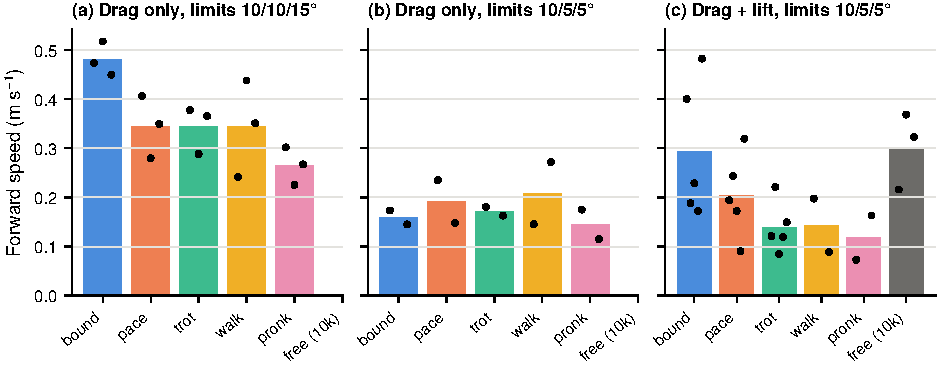
\includegraphics[width=\textwidth]{fig_mj_families}
  \caption[Fastest gaits per family in MuJoCo]{Fastest gait per family in the reduced-order model; bars are
    seed means, dots individual seeds. (a) Drag only, moderate limits. (b) Drag only, strict limits. (c) Drag and
    lift, strict limits, including three free-phase searches with $10^4$ evaluations. Free-phase searches with
    2500 evaluations are not shown because they had not converged.}
  \label{fig:mj-families}
\end{figure}

\section{Coordination with Lift under Strict Limits}

With lift and strict limits, all fifteen trot, pace and bound solutions over five seeds are lift-propelled,
feasible and do not surface (\cref{tab:mj-families}, \cref{fig:mj-families}c). Bound is again the fastest, up to
\SI{0.483}{\metre\per\second} for one seed, as fast as the fastest drag-only gait under moderate limits, but its
servos are saturated almost all the time. Trot has the lowest mean power ($1.23\pm\SI{0.90}{\watt}$) but is also the slowest of the three, so its low energy per metre mixes \enquote{economical} with \enquote{slow}.

To separate the two, the least power at equal speed was computed per family with lift and strict limits
(five seeds, \cref{fig:mj-coord}). At \SI{0.10}{\metre\per\second} trot needs \SI{0.10}{\watt} against
\SI{0.17}{\watt} for bound, and at \SI{0.15}{\metre\per\second} \SI{0.48}{} against \SI{0.51}{\watt}; the medians
over seeds are close. At \SI{0.20}{\metre\per\second} trot needs \SI{1.68}{\watt}, while pronk and bound need
\SI{0.96}{} and \SI{0.98}{\watt}, and only three of five trot seeds are feasible; trot's speed limit under strict
limits is about \SI{0.22}{\metre\per\second}. All 55 feasible solutions of this experiment are lift-propelled.
Diagonal coordination is therefore at most marginally more economical at low speed; above about
\SI{0.15}{\metre\per\second}, fore--aft coordinations are both more economical and faster.
\Cref{fig:mj-trot} shows one lift-propelled trot at \SI{0.221}{\metre\per\second} and \SI{1.03}{\watt}, whose
servos never saturate.

The free-phase search needs a larger budget. With 2500 evaluations it reached only
\SIrange{0.05}{0.07}{\metre\per\second}; with $10^4$ evaluations, three seeds reached
$0.303\pm\SI{0.078}{\metre\per\second}$, all lift-propelled and all converged to fore--aft coordinations close to
bound or pronk (deviation 15--19\,\% of a period), not to trot. The best free gait, \SI{0.369}{\metre\per\second}
at \SI{3.3}{\watt}, is faster than three of the five bound optima and needs less energy per metre than all five, which shows that better
coordinations exist outside the fixed families.

\begin{figure}[t]
  \centering
  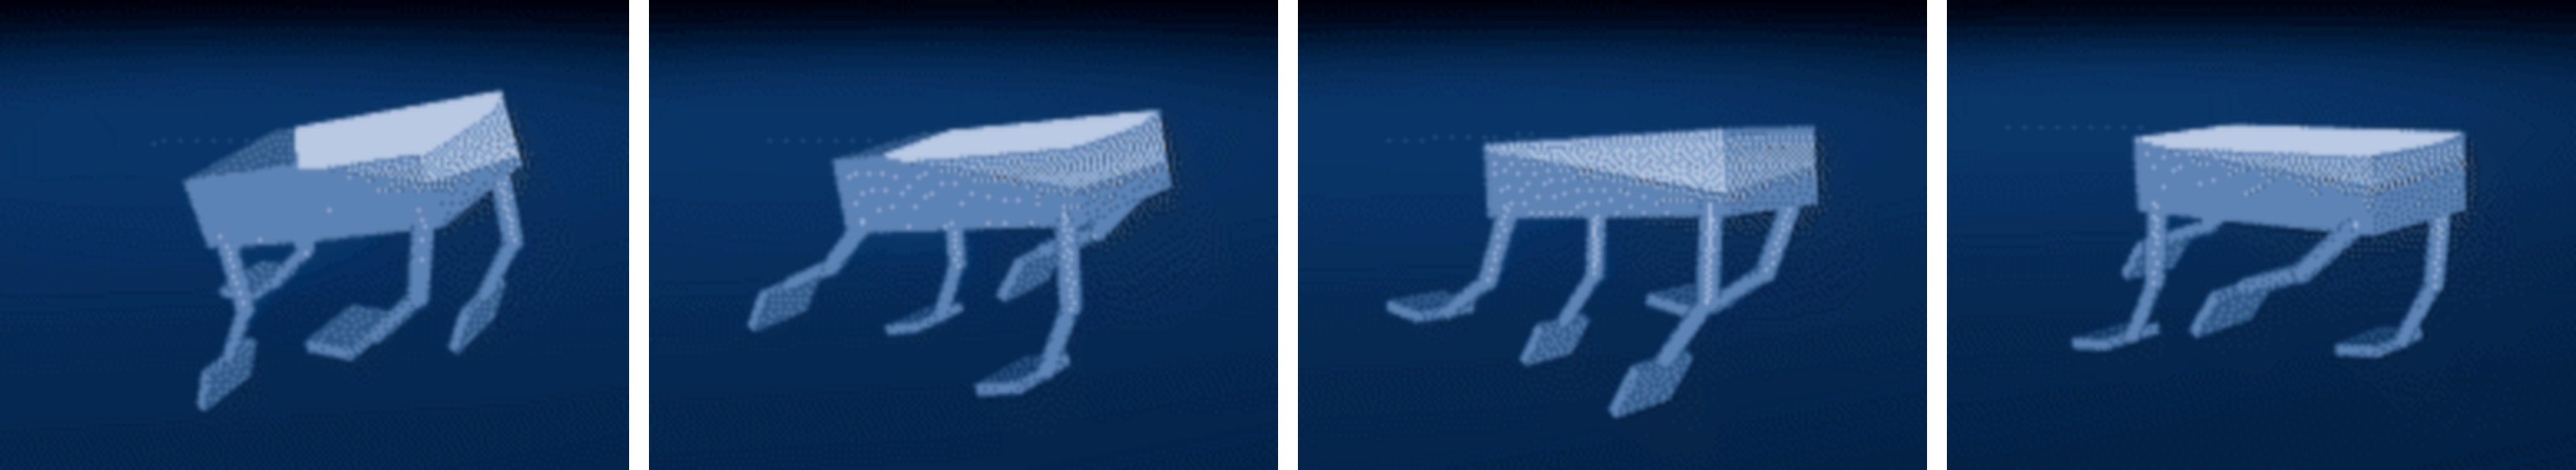
\includegraphics[width=\textwidth]{fig_mj_trot_frames.png}\\[1mm]
  {\small (a)}\\[2mm]
  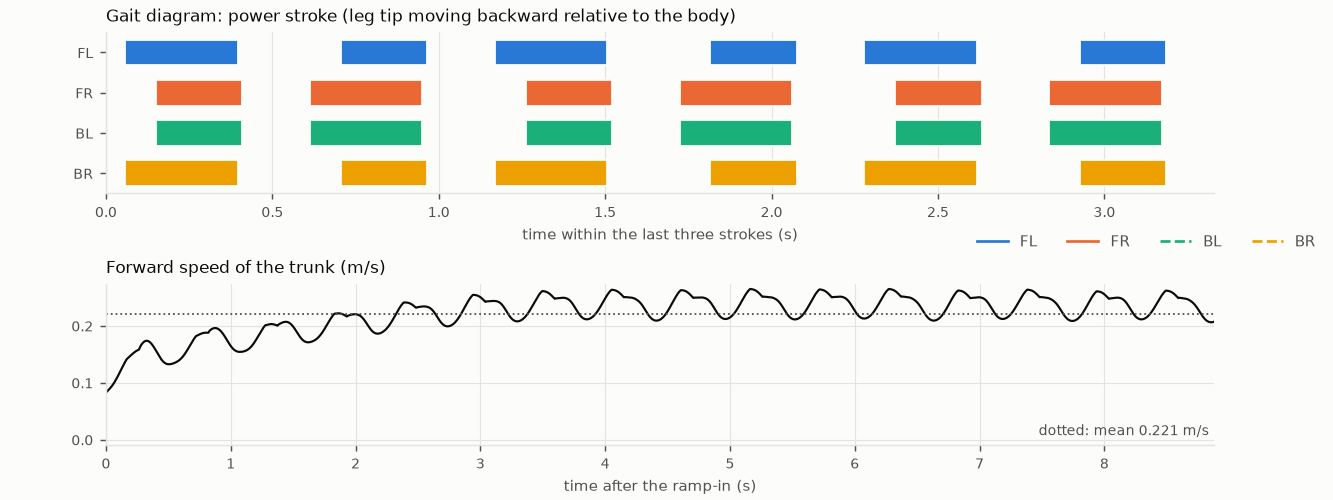
\includegraphics[width=\textwidth]{fig_mj_trot.png}\\
  {\small (b)}
  \caption[A lift-propelled trot in MuJoCo]{A lift-propelled trot found with strict limits (\SI{0.90}{\hertz},
    $\mathrm{DUTY}=0.59$, \SI{0.221}{\metre\per\second}, \SI{1.03}{\watt}). (a) Four frames of the MuJoCo animation,
    \SIrange{0.25}{0.30}{\second} apart, covering one stroke period of \SI{1.11}{\second}; the camera follows the trunk. (b) Top:
    power strokes of the four legs over the last three cycles; diagonal legs act together. Bottom: forward speed of the trunk
    after the ramp-in, mean dotted.}
  \label{fig:mj-trot}
\end{figure}


\begin{figure}[t]
  \centering
  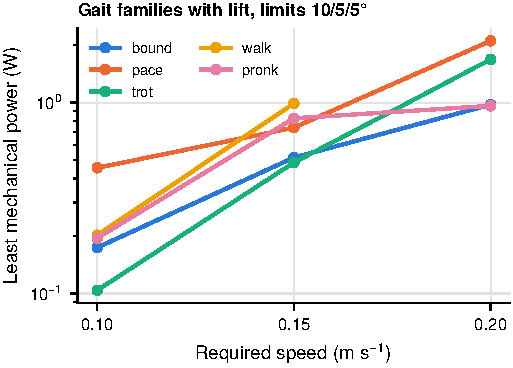
\includegraphics[width=0.58\textwidth]{fig_mj_coord}
  \caption[Least power per gait family]{Least mechanical power to reach a required speed per gait family, with lift and strict limits
    (best of five seeds).}
  \label{fig:mj-coord}
\end{figure}

\section{Electrical Power}

Because most of the fastest gaits keep their servos at the torque limit, the mechanical-power ranking could
hide large copper losses. The electrical power was therefore recomputed for all 222 valid optima. Averaged per family, it lies within about $\pm30$\,\% of the mechanical power, because at saturation the back-EMF term cancels much of the stall torque. The exceptions are trot and pronk with drag only under moderate limits, whose electrical power is 71\,\% and 44\,\% higher (for trot \SI{19.6}{} instead of \SI{11.5}{\watt}). This moves trot behind pace and walk in energy per metre; apart from this, the statements of this appendix hold for the electrical power as well.

\chapter{Real-Time Solver: Tow Runs and Whole-Robot Trends}
\label{app:flare-trends}

This appendix collects the Flare Live results. The tow runs are the basis of the cross-check in \cref{sec:ver-flare}; the
self-propelled runs show trends of the whole robot but no reliable magnitudes.

\section{Tow Runs}
\label{app:flare}

\begin{table}[H]
  \centering
  \caption[Flare Live tow runs]{Flare Live tow runs with the L0 motion: streamwise fluid force on the fluke (fluke frame) and net
    thrust of the whole flapping leg, in \si{\milli\newton}, averaged over $t=\SIrange{3}{9}{\second}$.}
  \label{tab:app-flare}
  \footnotesize
  \begin{tabular}{@{}lcccccc@{}}
    \toprule
    $\U$ (\si{\metre\per\second}) & Lattice & Fluke, flapping & Fluke, idle & Leg net thrust & CFD fluke & $\alpha_{75}$ \\
    \midrule
    0     & \SI{3}{\milli\metre} & 20.0  & --      & 25.7 & 45.5 & \SI{73.8}{\degree} \\
    0.1   & \SI{3}{\milli\metre} & 8.5   & --      & 15.9 & $\approx34$ & \SI{41.1}{\degree} \\
    0.223 & \SI{3}{\milli\metre} & $-0.1$ & $-12.6$ & 9.6  & 21.4 & \SI{19.7}{\degree} \\
    0.223 & \SI{2}{\milli\metre} & 4.1   & $-11.6$ & 5.8  & 21.4 & \SI{19.8}{\degree} \\
    \bottomrule
  \end{tabular}
\end{table}

\section{Self-Propelled Runs}

Because of the thrust deficit of \cref{sec:ver-flare}, the self-propelled Flare Live runs are used only for trends
(\cref{fig:flare-robot}, \cref{tab:flare}). With the resistance $K=\SI{0.65}{\newton\second\squared\per\metre\squared}$
($D_\text{mid}$), a trot at \SI{2}{\hertz} with a target angle of attack of \SI{18}{\degree} swims at
\SI{0.154}{\metre\per\second}, about half the CFD-based prediction, consistent with the missing fluke thrust.
\begin{itemize}
  \item \emph{Frequency.} Speed grows with frequency as $\U\propto f^{0.71}$ at $K=0.65$ ($f^{0.51}$ at $K=3.95$), while power grows
        as $f^{1.8}$; the cost of transport rises with frequency. The Strouhal number stays nearly constant.
  \item \emph{Angle of attack.} The target \SI{18}{\degree} gives the highest speed and the lowest cost of transport; \SI{28}{\degree}
        is slightly slower, \SI{10}{\degree} much slower. The controller does hold the target: in the \SI{10}{\degree} run, the
        mid-stroke angle of attack has a median of \SI{10.1}{\degree}, but the fluke has to rotate by \SI{122}{\degree} per cycle and
        sits at its end stop 11\,\% of the time. In CFD, the \SI{10}{\degree} law gave the most thrust at this speed
        (\cref{sec:res-lift}). The penalty for small angles in Flare Live is consistent with its unresolved lift; only the statement
        that efficiency is highest near \SIrange{18}{20}{\degree} is supported by both solvers.
  \item \emph{Resistance.} Lowering $K$ from 0.65 to 0.27 (bare hull) raises the speed only from \SI{0.154}{} to
        \SI{0.160}{\metre\per\second}, so in Flare Live the robot is limited by its thrust rather than by its hull.
  \item \emph{Attitude.} The hull heaves by less than \SI{0.6}{\milli\metre} and pitches by less than \SI{0.3}{\degree} in the trot:
        diagonal coordination keeps the floating robot level.
\end{itemize}

\begin{table}[t]
  \centering
  \caption[Flare Live self-propelled runs]{Self-propelled Flare Live runs, trot, $K=\SI{0.65}{\newton\second\squared\per\metre\squared}$.
    COT $=P_\text{j}/(mg\U)$ with the joint-drive power $P_\text{j}$ and $m=\SI{0.863}{\kilo\gram}$.}
  \label{tab:flare}
  \small
  \begin{tabular}{@{}lccc@{}}
    \toprule
    Run & $\U$ (\si{\milli\metre\per\second}) & $P_\text{j}$ (mW) & COT \\
    \midrule
    \SI{2}{\hertz}, $\alpha$ \SI{10}{\degree} & 100.2 & 261 & 0.31 \\
    \SI{2}{\hertz}, $\alpha$ \SI{18}{\degree} & \textbf{153.8} & 239 & \textbf{0.18} \\
    \SI{2}{\hertz}, $\alpha$ \SI{28}{\degree} & 143.8 & 249 & 0.20 \\
    \SI{2.5}{\hertz}, $\alpha$ \SI{18}{\degree} & 183.1 & 355 & 0.23 \\
    \SI{3}{\hertz}, $\alpha$ \SI{18}{\degree} & 205.0 & 488 & 0.28 \\
    \bottomrule
  \end{tabular}
\end{table}

\begin{figure}[t]
  \centering
  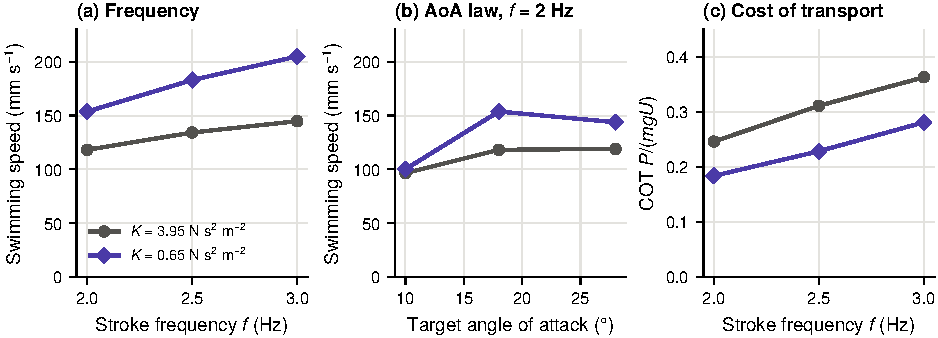
\includegraphics[width=\textwidth]{fig_flare_robot}
  \caption[Flare Live free-swimming trends]{Self-propelled robot in Flare Live (trot). (a) Speed versus stroke frequency for two
    hull resistances. (b) Speed versus the target angle of attack at \SI{2}{\hertz}. (c) Cost of transport versus frequency.}
  \label{fig:flare-robot}
\end{figure}

The joint-drive power in Flare Live (\SIrange{240}{490}{\milli\watt}) is an order of magnitude above the hydrodynamic power of
the CFD (about \SI{65}{\milli\watt} for four flukes), because it includes the power to move the linkages, their inertia and the
controller effort.

\chapter{Reproducibility}
\label{app:repro}

\section{Software}

\begin{sloppypar}
\begin{itemize}
  \item OpenFOAM v2606, \texttt{overPimpleDyMFoam}; meshes with \texttt{blockMesh} and \texttt{snappyHexMesh}. Case generators,
        run scripts and post-processing in Python (\texttt{make\_leg\_cfd.py}, \texttt{make\_fluke\_cfd.py},
        \texttt{fluke\_traj.py}, \texttt{fluke\_forces.py}).
  \item MuJoCo 3.14 with the Python package \texttt{cma}; the gait-optimization code \texttt{swimopt} (\url{https://github.com/lxtuni/swimopt}), including the raw results of all
        234 runs, 222 of them valid (\texttt{thesis\_notes/data/all\_runs.csv}). The replay of the drag-only optima with lift
        (\cref{sec:mj-liftshare}) is documented in the notes of the repository, not in \texttt{all\_runs.csv}.
  \item Flare Live with the scripts \texttt{run\_float.py} (self-propelled runs) and \texttt{bench\_foil.py} (tow runs).
\end{itemize}
\end{sloppypar}
\TODO{Add the repository of the CFD and Flare Live scripts and the commit hashes of the final versions.}

\section{MuJoCo Settings}

\begin{table}[H]
  \centering
  \caption[MuJoCo settings]{Settings of the reduced-order gait optimization.}
  \label{tab:app-mujoco}
  \small
  \begin{tabularx}{\textwidth}{@{}l>{\raggedright\arraybackslash}X@{}}
    \toprule
    Item & Value \\
    \midrule
    Time step, integrator & \SI{2}{\milli\second}, implicit-fast \\
    Evaluation & settle \SI{1.0}{\second}, ramp-in \SI{1.5}{\second}, score \SI{8}{\second} rounded up to whole periods \\
    Servo & position servo, stiffness 60, critical damping, $\tau_s=\SI{3}{\newton\metre}$, $\omega_\text{max}=\SI{400}{\degree\per\second}$ \\
    Flipper coefficients & $C_D=(2.2,0.10,0.10)$, $C_a=1.0$, $c_v=0.05$, $c_l=1.1$ \\
    Link coefficients & $C_D=(0.5,0.5,0.25)$, $C_a=0.3$, $c_v=0.02$ \\
    Trunk coefficients & $C_D=(0.9,1.6,1.8)$, $C_a=0.2$, $c_v=0.10$ \\
    Gait & $H=2$; $f\in[0.2,2.5]$\,Hz; DUTY $\in[0.25,0.75]$; $A\in[0,0.9]$\,rad; $q_0\in[-0.5,0.5]$\,rad \\
    CMA-ES & population 16, $\sigma_0=0.25$, 2500 evaluations ($10^4$ for free phase), non-zero seeds \\
    Limits & heading/roll/pitch RMS $10/10/\SI{15}{\degree}$ or $10/5/\SI{5}{\degree}$; surfacing $\le5$\,\% where stated; lift thrust share $s_L\le0.1$ for the drag-based strokes of \cref{sec:mj-liftshare} \\
    \bottomrule
  \end{tabularx}
\end{table}

\section{Model Errors Found and Corrected}

Several errors in the simulation set-up were found during the work and corrected before the reported results were produced.
They are listed because they are easy to repeat.
\begin{itemize}
  \item MJCF reads joint ranges in degrees by default; a range of $\pm1.3$ intended in radians locked every joint to
        $\pm\SI{1.3}{\degree}$. All results before this correction were discarded.
  \item Changing body masses at run time without recomputing MuJoCo's derived constants made the added mass ineffective for a
        single free body and caused a 36\,\% error in a momentum-conservation test.
  \item Visual and collision geometries imported from a URDF were both given hydrodynamic forces, doubling buoyancy, drag and added
        mass.
  \item An additive weighting of speed and attitude produced strongly rolling and yawing optima once the legs could move freely;
        it was replaced by the feasibility-first formulation \eqref{eq:feasibility}.
  \item A first measure of the lift share, $|I_L|/(|I_L|+|I_\text{drag}|)$, is about 0.5 for every gait with lift, because in steady
        swimming the lift and drag impulses cancel. Used as a limit, it could only be met by gaits that barely moved. It was
        replaced by $s_L$ of \eqref{eq:liftshare}, and the runs with the old measure were discarded.
  \item In the fluke CFD, a coarse background mesh that had not been refined around the fluke led to a failed hole cutting in which
        almost the whole background was removed; the number of hole cells is now checked automatically.
\end{itemize}


\printbibliography[heading=bibintoc,title={Bibliography}]
\end{document}
